% Options for packages loaded elsewhere
\PassOptionsToPackage{unicode}{hyperref}
\PassOptionsToPackage{hyphens}{url}
%
\documentclass[
]{book}
\usepackage{amsmath,amssymb}
\usepackage{lmodern}
\usepackage{iftex}
\ifPDFTeX
  \usepackage[T1]{fontenc}
  \usepackage[utf8]{inputenc}
  \usepackage{textcomp} % provide euro and other symbols
\else % if luatex or xetex
  \usepackage{unicode-math}
  \defaultfontfeatures{Scale=MatchLowercase}
  \defaultfontfeatures[\rmfamily]{Ligatures=TeX,Scale=1}
\fi
% Use upquote if available, for straight quotes in verbatim environments
\IfFileExists{upquote.sty}{\usepackage{upquote}}{}
\IfFileExists{microtype.sty}{% use microtype if available
  \usepackage[]{microtype}
  \UseMicrotypeSet[protrusion]{basicmath} % disable protrusion for tt fonts
}{}
\makeatletter
\@ifundefined{KOMAClassName}{% if non-KOMA class
  \IfFileExists{parskip.sty}{%
    \usepackage{parskip}
  }{% else
    \setlength{\parindent}{0pt}
    \setlength{\parskip}{6pt plus 2pt minus 1pt}}
}{% if KOMA class
  \KOMAoptions{parskip=half}}
\makeatother
\usepackage{xcolor}
\IfFileExists{xurl.sty}{\usepackage{xurl}}{} % add URL line breaks if available
\IfFileExists{bookmark.sty}{\usepackage{bookmark}}{\usepackage{hyperref}}
\hypersetup{
  pdftitle={数据科学导论(Introductory of Data Science)},
  pdfauthor={潘蓄林},
  hidelinks,
  pdfcreator={LaTeX via pandoc}}
\urlstyle{same} % disable monospaced font for URLs
\usepackage{color}
\usepackage{fancyvrb}
\newcommand{\VerbBar}{|}
\newcommand{\VERB}{\Verb[commandchars=\\\{\}]}
\DefineVerbatimEnvironment{Highlighting}{Verbatim}{commandchars=\\\{\}}
% Add ',fontsize=\small' for more characters per line
\usepackage{framed}
\definecolor{shadecolor}{RGB}{248,248,248}
\newenvironment{Shaded}{\begin{snugshade}}{\end{snugshade}}
\newcommand{\AlertTok}[1]{\textcolor[rgb]{0.94,0.16,0.16}{#1}}
\newcommand{\AnnotationTok}[1]{\textcolor[rgb]{0.56,0.35,0.01}{\textbf{\textit{#1}}}}
\newcommand{\AttributeTok}[1]{\textcolor[rgb]{0.77,0.63,0.00}{#1}}
\newcommand{\BaseNTok}[1]{\textcolor[rgb]{0.00,0.00,0.81}{#1}}
\newcommand{\BuiltInTok}[1]{#1}
\newcommand{\CharTok}[1]{\textcolor[rgb]{0.31,0.60,0.02}{#1}}
\newcommand{\CommentTok}[1]{\textcolor[rgb]{0.56,0.35,0.01}{\textit{#1}}}
\newcommand{\CommentVarTok}[1]{\textcolor[rgb]{0.56,0.35,0.01}{\textbf{\textit{#1}}}}
\newcommand{\ConstantTok}[1]{\textcolor[rgb]{0.00,0.00,0.00}{#1}}
\newcommand{\ControlFlowTok}[1]{\textcolor[rgb]{0.13,0.29,0.53}{\textbf{#1}}}
\newcommand{\DataTypeTok}[1]{\textcolor[rgb]{0.13,0.29,0.53}{#1}}
\newcommand{\DecValTok}[1]{\textcolor[rgb]{0.00,0.00,0.81}{#1}}
\newcommand{\DocumentationTok}[1]{\textcolor[rgb]{0.56,0.35,0.01}{\textbf{\textit{#1}}}}
\newcommand{\ErrorTok}[1]{\textcolor[rgb]{0.64,0.00,0.00}{\textbf{#1}}}
\newcommand{\ExtensionTok}[1]{#1}
\newcommand{\FloatTok}[1]{\textcolor[rgb]{0.00,0.00,0.81}{#1}}
\newcommand{\FunctionTok}[1]{\textcolor[rgb]{0.00,0.00,0.00}{#1}}
\newcommand{\ImportTok}[1]{#1}
\newcommand{\InformationTok}[1]{\textcolor[rgb]{0.56,0.35,0.01}{\textbf{\textit{#1}}}}
\newcommand{\KeywordTok}[1]{\textcolor[rgb]{0.13,0.29,0.53}{\textbf{#1}}}
\newcommand{\NormalTok}[1]{#1}
\newcommand{\OperatorTok}[1]{\textcolor[rgb]{0.81,0.36,0.00}{\textbf{#1}}}
\newcommand{\OtherTok}[1]{\textcolor[rgb]{0.56,0.35,0.01}{#1}}
\newcommand{\PreprocessorTok}[1]{\textcolor[rgb]{0.56,0.35,0.01}{\textit{#1}}}
\newcommand{\RegionMarkerTok}[1]{#1}
\newcommand{\SpecialCharTok}[1]{\textcolor[rgb]{0.00,0.00,0.00}{#1}}
\newcommand{\SpecialStringTok}[1]{\textcolor[rgb]{0.31,0.60,0.02}{#1}}
\newcommand{\StringTok}[1]{\textcolor[rgb]{0.31,0.60,0.02}{#1}}
\newcommand{\VariableTok}[1]{\textcolor[rgb]{0.00,0.00,0.00}{#1}}
\newcommand{\VerbatimStringTok}[1]{\textcolor[rgb]{0.31,0.60,0.02}{#1}}
\newcommand{\WarningTok}[1]{\textcolor[rgb]{0.56,0.35,0.01}{\textbf{\textit{#1}}}}
\usepackage{longtable,booktabs,array}
\usepackage{calc} % for calculating minipage widths
% Correct order of tables after \paragraph or \subparagraph
\usepackage{etoolbox}
\makeatletter
\patchcmd\longtable{\par}{\if@noskipsec\mbox{}\fi\par}{}{}
\makeatother
% Allow footnotes in longtable head/foot
\IfFileExists{footnotehyper.sty}{\usepackage{footnotehyper}}{\usepackage{footnote}}
\makesavenoteenv{longtable}
\usepackage{graphicx}
\makeatletter
\def\maxwidth{\ifdim\Gin@nat@width>\linewidth\linewidth\else\Gin@nat@width\fi}
\def\maxheight{\ifdim\Gin@nat@height>\textheight\textheight\else\Gin@nat@height\fi}
\makeatother
% Scale images if necessary, so that they will not overflow the page
% margins by default, and it is still possible to overwrite the defaults
% using explicit options in \includegraphics[width, height, ...]{}
\setkeys{Gin}{width=\maxwidth,height=\maxheight,keepaspectratio}
% Set default figure placement to htbp
\makeatletter
\def\fps@figure{htbp}
\makeatother
\setlength{\emergencystretch}{3em} % prevent overfull lines
\providecommand{\tightlist}{%
  \setlength{\itemsep}{0pt}\setlength{\parskip}{0pt}}
\setcounter{secnumdepth}{5}
\usepackage{booktabs}
\usepackage{amsthm}
\makeatletter
\def\thm@space@setup{%
  \thm@preskip=8pt plus 2pt minus 4pt
  \thm@postskip=\thm@preskip
}
\makeatother
\ifLuaTeX
  \usepackage{selnolig}  % disable illegal ligatures
\fi
\usepackage[]{natbib}
\bibliographystyle{apalike}

\title{数据科学导论(Introductory of Data Science)}
\author{潘蓄林}
\date{2022-04-12}

\begin{document}
\maketitle

{
\setcounter{tocdepth}{1}
\tableofcontents
}
\hypertarget{ux524dux8a00prerequisites}{%
\chapter{前言(Prerequisites)}\label{ux524dux8a00prerequisites}}

数据科学:从数据中提取出有价值的知识。

数据:主要指大数据,符合``4V+C''(Value,Variatey,Volumn,Velocity,Complex)特征的数据;

\hypertarget{rux53capythonux8bedux8a00ux7b80ux4ecb}{%
\chapter{R及Python语言简介}\label{rux53capythonux8bedux8a00ux7b80ux4ecb}}

\hypertarget{rux7b80ux4ecb}{%
\subsection{R简介}\label{rux7b80ux4ecb}}

\begin{enumerate}
\def\labelenumi{\arabic{enumi}.}
\tightlist
\item
  R语言是从S统计绘图语言演变而来, 可看作S的``方言'';
\item
  S语言诞生于上世纪70年代的贝尔实验室, 由Rick Becker, John Chambers, Allan Wilks开发; 基于S语言开发的商业软件Splus, 可以方便的编写函数、建立模型, 具有良好的扩展性, 在国外学术界应用很广.
\item
  1995年, 新西兰Auckland大学统计系的Robert Gentleman和Ross Ihaka, 基于S语言的源代码, 编写了能执行S语言的软件, 并将该软件的源代码全部公开, 这就是R软件, 其命令统称为R语言.
\end{enumerate}

\hypertarget{rux8bedux8a00ux5b89ux88c5ux53caux73afux5883ux914dux7f6e}{%
\subsection{R语言安装及环境配置}\label{rux8bedux8a00ux5b89ux88c5ux53caux73afux5883ux914dux7f6e}}

\begin{itemize}
\tightlist
\item
  下载R:
  \href{https://www.r-project.org/}{R官方网站}
\end{itemize}

\begin{enumerate}
\def\labelenumi{\arabic{enumi}.}
\tightlist
\item
  选择合适的源;
\item
  根据操作系统选择合适的包下载
\end{enumerate}

\begin{itemize}
\tightlist
\item
  安装r软件;
\end{itemize}

\hypertarget{rstudioux8f6fux4ef6ux5b89ux88c5}{%
\subsection{Rstudio软件安装}\label{rstudioux8f6fux4ef6ux5b89ux88c5}}

\begin{itemize}
\tightlist
\item
  下载Rstudio:
  \href{https://www.rstudio.com/products/rstudio/download/}{Rstudio官方网站}
\end{itemize}

\begin{enumerate}
\def\labelenumi{\arabic{enumi}.}
\tightlist
\item
  选择free的下载;
\item
  根据操作系统选择合适的包下载
\end{enumerate}

\begin{itemize}
\item
  安装r软件;
\item
  R语言安装(win版):\href{https://cran.r-project.org/bin/windows/base/R-3.6.1-win.exe}{下载软件}
\item
  双击,按照提示完成安装(使用默认安装)
\item
  Rstudio安装:Studio是R最佳的图形编辑环境
\end{itemize}

\hypertarget{rux57faux7840}{%
\subsection{R基础}\label{rux57faux7840}}

\begin{Shaded}
\begin{Highlighting}[]
\CommentTok{\#试试R编程 }
\NormalTok{x}\OtherTok{=}\DecValTok{1}\SpecialCharTok{:}\DecValTok{100}\CommentTok{\#把1,2,...,100这个整数向量赋值到x}
\NormalTok{(}\AttributeTok{x=}\DecValTok{1}\SpecialCharTok{:}\DecValTok{100}\NormalTok{) }\CommentTok{\#同上, 只不过显示出来}
\end{Highlighting}
\end{Shaded}

\begin{verbatim}
##   [1]   1   2   3   4   5   6   7   8   9  10  11  12  13  14  15  16  17  18
##  [19]  19  20  21  22  23  24  25  26  27  28  29  30  31  32  33  34  35  36
##  [37]  37  38  39  40  41  42  43  44  45  46  47  48  49  50  51  52  53  54
##  [55]  55  56  57  58  59  60  61  62  63  64  65  66  67  68  69  70  71  72
##  [73]  73  74  75  76  77  78  79  80  81  82  83  84  85  86  87  88  89  90
##  [91]  91  92  93  94  95  96  97  98  99 100
\end{verbatim}

\begin{Shaded}
\begin{Highlighting}[]
\FunctionTok{sample}\NormalTok{(x,}\DecValTok{20}\NormalTok{) }\CommentTok{\#从1,2,...,100中随机不放回地抽取20个值作为样本}
\end{Highlighting}
\end{Shaded}

\begin{verbatim}
##  [1]  82  85  25  11  12  95  99  43  10  13 100   7  92  68  49  21  73  18  33
## [20]  84
\end{verbatim}

\begin{Shaded}
\begin{Highlighting}[]
\FunctionTok{set.seed}\NormalTok{(}\DecValTok{0}\NormalTok{);}\FunctionTok{sample}\NormalTok{(}\DecValTok{1}\SpecialCharTok{:}\DecValTok{10}\NormalTok{,}\DecValTok{3}\NormalTok{)}\CommentTok{\#先设随机种子再抽样}
\end{Highlighting}
\end{Shaded}

\begin{verbatim}
## [1] 9 4 7
\end{verbatim}

\begin{Shaded}
\begin{Highlighting}[]
\CommentTok{\#从1,2,...,200000中随机不放回地抽取10000个值作为样本:}
\NormalTok{z}\OtherTok{=}\FunctionTok{sample}\NormalTok{(}\DecValTok{1}\SpecialCharTok{:}\DecValTok{20}\NormalTok{,}\DecValTok{5}\NormalTok{)}
\NormalTok{z[}\DecValTok{1}\SpecialCharTok{:}\DecValTok{3}\NormalTok{]}\CommentTok{\#方括号中为向量z的下标}
\end{Highlighting}
\end{Shaded}

\begin{verbatim}
## [1]  1  2 11
\end{verbatim}

\begin{Shaded}
\begin{Highlighting}[]
\NormalTok{y}\OtherTok{=}\FunctionTok{c}\NormalTok{(}\DecValTok{1}\NormalTok{,}\DecValTok{3}\NormalTok{,}\DecValTok{7}\NormalTok{,}\DecValTok{3}\NormalTok{,}\DecValTok{4}\NormalTok{,}\DecValTok{2}\NormalTok{)}
\NormalTok{z[y]}\CommentTok{\#以y为下标的z的元素值}
\end{Highlighting}
\end{Shaded}

\begin{verbatim}
## [1]  1 11 NA 11 14  2
\end{verbatim}

\begin{Shaded}
\begin{Highlighting}[]
\NormalTok{(}\AttributeTok{z=}\FunctionTok{sample}\NormalTok{(x,}\DecValTok{100}\NormalTok{,}\AttributeTok{rep=}\NormalTok{T))}\CommentTok{\#从x有放回地随机抽取100个值作为样本}
\end{Highlighting}
\end{Shaded}

\begin{verbatim}
##   [1]  59  51  97  85  21  54  74   7  73  79  85  37  89  37  34  89  44  79
##  [19]  33  84  35  70  74  42  38  20  28  20  44  87  70  40  44  25  70  39
##  [37]  51  42   6  24  32  14   2  45  18  22  78  65  70  87  70  75  81 100
##  [55]  13  40  89  48  89  23  84  29  13  22  93  28  48  33  45  21  31  17
##  [73]  73  87  83  90  48  64  94  96  60  51  93  34  10   1  43  59  26  15
##  [91]  58  29  24  42  48  76  39  24  53  92
\end{verbatim}

\begin{Shaded}
\begin{Highlighting}[]
\NormalTok{(}\AttributeTok{z1=}\FunctionTok{unique}\NormalTok{(z))}
\end{Highlighting}
\end{Shaded}

\begin{verbatim}
##  [1]  59  51  97  85  21  54  74   7  73  79  37  89  34  44  33  84  35  70  42
## [20]  38  20  28  87  40  25  39   6  24  32  14   2  45  18  22  78  65  75  81
## [39] 100  13  48  23  29  93  31  17  83  90  64  94  96  60  10   1  43  26  15
## [58]  58  76  53  92
\end{verbatim}

\begin{Shaded}
\begin{Highlighting}[]
\FunctionTok{length}\NormalTok{(z1)}\CommentTok{\#z中不同元素的个数}
\end{Highlighting}
\end{Shaded}

\begin{verbatim}
## [1] 61
\end{verbatim}

\begin{Shaded}
\begin{Highlighting}[]
\NormalTok{xz}\OtherTok{=}\FunctionTok{setdiff}\NormalTok{(x,z) }\CommentTok{\#x和z之间的不同元素{-}{-}集合差}
\FunctionTok{sort}\NormalTok{(}\FunctionTok{union}\NormalTok{(xz,z))}\CommentTok{\#对xz及z的并的元素从小到大排序}
\end{Highlighting}
\end{Shaded}

\begin{verbatim}
##   [1]   1   2   3   4   5   6   7   8   9  10  11  12  13  14  15  16  17  18
##  [19]  19  20  21  22  23  24  25  26  27  28  29  30  31  32  33  34  35  36
##  [37]  37  38  39  40  41  42  43  44  45  46  47  48  49  50  51  52  53  54
##  [55]  55  56  57  58  59  60  61  62  63  64  65  66  67  68  69  70  71  72
##  [73]  73  74  75  76  77  78  79  80  81  82  83  84  85  86  87  88  89  90
##  [91]  91  92  93  94  95  96  97  98  99 100
\end{verbatim}

\begin{Shaded}
\begin{Highlighting}[]
\FunctionTok{setequal}\NormalTok{(}\FunctionTok{union}\NormalTok{(xz,z),x) }\CommentTok{\#xz及z的并的元素与x是否一样}
\end{Highlighting}
\end{Shaded}

\begin{verbatim}
## [1] TRUE
\end{verbatim}

\begin{Shaded}
\begin{Highlighting}[]
\FunctionTok{intersect}\NormalTok{(}\DecValTok{1}\SpecialCharTok{:}\DecValTok{10}\NormalTok{,}\DecValTok{7}\SpecialCharTok{:}\DecValTok{50}\NormalTok{) }\CommentTok{\#两个数据的交}
\end{Highlighting}
\end{Shaded}

\begin{verbatim}
## [1]  7  8  9 10
\end{verbatim}

\begin{Shaded}
\begin{Highlighting}[]
\FunctionTok{sample}\NormalTok{(}\DecValTok{1}\SpecialCharTok{:}\DecValTok{100}\NormalTok{,}\DecValTok{20}\NormalTok{,}\AttributeTok{prob=}\DecValTok{1}\SpecialCharTok{:}\DecValTok{100}\NormalTok{)}\CommentTok{\#从1:100中不等概率随机抽样,}
\end{Highlighting}
\end{Shaded}

\begin{verbatim}
##  [1] 91 50 95 36 62 67 82 74 70 90 66 97 84 87 81 29 71 43 31 75
\end{verbatim}

\begin{Shaded}
\begin{Highlighting}[]
\CommentTok{\#上一语句各数字被抽到的概率与其值大小成比例}
\NormalTok{pi}\SpecialCharTok{*}\DecValTok{10}\SpecialCharTok{\^{}}\DecValTok{2} \CommentTok{\#能够用?"*"、?"\^{}"等来看某些基本算子的帮助, pi是圆周率}
\end{Highlighting}
\end{Shaded}

\begin{verbatim}
## [1] 314.1593
\end{verbatim}

\begin{Shaded}
\begin{Highlighting}[]
\StringTok{"*"}\NormalTok{(pi,}\StringTok{"\^{}"}\NormalTok{(}\DecValTok{10}\NormalTok{,}\DecValTok{2}\NormalTok{)) }\CommentTok{\#和上面一样, 有些烦琐, 是吧! 没有人这么用}
\end{Highlighting}
\end{Shaded}

\begin{verbatim}
## [1] 314.1593
\end{verbatim}

\begin{Shaded}
\begin{Highlighting}[]
\NormalTok{pi}\SpecialCharTok{*}\NormalTok{(}\DecValTok{1}\SpecialCharTok{:}\DecValTok{10}\NormalTok{)}\SpecialCharTok{\^{}{-}}\FloatTok{2.3}\CommentTok{\#可以对向量求指数幂}
\end{Highlighting}
\end{Shaded}

\begin{verbatim}
##  [1] 3.14159265 0.63794154 0.25105622 0.12954239 0.07753876 0.05098025
##  [7] 0.03576221 0.02630528 0.02006283 0.01574526
\end{verbatim}

\begin{Shaded}
\begin{Highlighting}[]
\NormalTok{x }\OtherTok{=}\NormalTok{ pi }\SpecialCharTok{*} \DecValTok{10}\SpecialCharTok{\^{}}\DecValTok{2}\NormalTok{ ; }\FunctionTok{print}\NormalTok{(x) }
\end{Highlighting}
\end{Shaded}

\begin{verbatim}
## [1] 314.1593
\end{verbatim}

\begin{Shaded}
\begin{Highlighting}[]
\NormalTok{(}\AttributeTok{x=}\NormalTok{pi }\SpecialCharTok{*}\DecValTok{10}\SpecialCharTok{\^{}}\DecValTok{2}\NormalTok{) }\CommentTok{\#赋值带打印}
\end{Highlighting}
\end{Shaded}

\begin{verbatim}
## [1] 314.1593
\end{verbatim}

\begin{Shaded}
\begin{Highlighting}[]
\NormalTok{pi}\SpecialCharTok{\^{}}\NormalTok{(}\DecValTok{1}\SpecialCharTok{:}\DecValTok{5}\NormalTok{) }\CommentTok{\#指数也可以是向量}
\end{Highlighting}
\end{Shaded}

\begin{verbatim}
## [1]   3.141593   9.869604  31.006277  97.409091 306.019685
\end{verbatim}

\begin{Shaded}
\begin{Highlighting}[]
\FunctionTok{print}\NormalTok{(x, }\AttributeTok{digits=} \DecValTok{12}\NormalTok{)}\CommentTok{\#输出x的12位数字}
\end{Highlighting}
\end{Shaded}

\begin{verbatim}
## [1] 314.159265359
\end{verbatim}

\begin{Shaded}
\begin{Highlighting}[]
\CommentTok{\#R对象的类型}
\NormalTok{x}\OtherTok{=}\NormalTok{pi}\SpecialCharTok{*}\DecValTok{10}\SpecialCharTok{\^{}}\DecValTok{2}
\FunctionTok{class}\NormalTok{(x) }\CommentTok{\#x的class}
\end{Highlighting}
\end{Shaded}

\begin{verbatim}
## [1] "numeric"
\end{verbatim}

\begin{Shaded}
\begin{Highlighting}[]
\FunctionTok{typeof}\NormalTok{(x) }\CommentTok{\#x的type}
\end{Highlighting}
\end{Shaded}

\begin{verbatim}
## [1] "double"
\end{verbatim}

\begin{Shaded}
\begin{Highlighting}[]
\FunctionTok{class}\NormalTok{(cars)}\CommentTok{\#cars是一个R中自带的数据}
\end{Highlighting}
\end{Shaded}

\begin{verbatim}
## [1] "data.frame"
\end{verbatim}

\begin{Shaded}
\begin{Highlighting}[]
\FunctionTok{typeof}\NormalTok{(cars) }\CommentTok{\#cars的type}
\end{Highlighting}
\end{Shaded}

\begin{verbatim}
## [1] "list"
\end{verbatim}

\begin{Shaded}
\begin{Highlighting}[]
\FunctionTok{names}\NormalTok{(cars)}\CommentTok{\#cars数据的变量名字}
\end{Highlighting}
\end{Shaded}

\begin{verbatim}
## [1] "speed" "dist"
\end{verbatim}

\begin{Shaded}
\begin{Highlighting}[]
\FunctionTok{summary}\NormalTok{(cars) }\CommentTok{\#cars的汇总}
\end{Highlighting}
\end{Shaded}

\begin{verbatim}
##      speed           dist       
##  Min.   : 4.0   Min.   :  2.00  
##  1st Qu.:12.0   1st Qu.: 26.00  
##  Median :15.0   Median : 36.00  
##  Mean   :15.4   Mean   : 42.98  
##  3rd Qu.:19.0   3rd Qu.: 56.00  
##  Max.   :25.0   Max.   :120.00
\end{verbatim}

\begin{Shaded}
\begin{Highlighting}[]
\FunctionTok{head}\NormalTok{(cars)}\CommentTok{\#cars的头几行数据, 和cars[1:6,]相同}
\end{Highlighting}
\end{Shaded}

\begin{verbatim}
##   speed dist
## 1     4    2
## 2     4   10
## 3     7    4
## 4     7   22
## 5     8   16
## 6     9   10
\end{verbatim}

\begin{Shaded}
\begin{Highlighting}[]
\FunctionTok{tail}\NormalTok{(cars) }\CommentTok{\#cars的最后几行数据}
\end{Highlighting}
\end{Shaded}

\begin{verbatim}
##    speed dist
## 45    23   54
## 46    24   70
## 47    24   92
## 48    24   93
## 49    24  120
## 50    25   85
\end{verbatim}

\begin{Shaded}
\begin{Highlighting}[]
\FunctionTok{str}\NormalTok{(cars)}\CommentTok{\#也是汇总}
\end{Highlighting}
\end{Shaded}

\begin{verbatim}
## 'data.frame':    50 obs. of  2 variables:
##  $ speed: num  4 4 7 7 8 9 10 10 10 11 ...
##  $ dist : num  2 10 4 22 16 10 18 26 34 17 ...
\end{verbatim}

\begin{Shaded}
\begin{Highlighting}[]
\FunctionTok{row.names}\NormalTok{(cars) }\CommentTok{\#行名字}
\end{Highlighting}
\end{Shaded}

\begin{verbatim}
##  [1] "1"  "2"  "3"  "4"  "5"  "6"  "7"  "8"  "9"  "10" "11" "12" "13" "14" "15"
## [16] "16" "17" "18" "19" "20" "21" "22" "23" "24" "25" "26" "27" "28" "29" "30"
## [31] "31" "32" "33" "34" "35" "36" "37" "38" "39" "40" "41" "42" "43" "44" "45"
## [46] "46" "47" "48" "49" "50"
\end{verbatim}

\begin{Shaded}
\begin{Highlighting}[]
\FunctionTok{attributes}\NormalTok{(cars)}\CommentTok{\#cars的一些信息}
\end{Highlighting}
\end{Shaded}

\begin{verbatim}
## $names
## [1] "speed" "dist" 
## 
## $class
## [1] "data.frame"
## 
## $row.names
##  [1]  1  2  3  4  5  6  7  8  9 10 11 12 13 14 15 16 17 18 19 20 21 22 23 24 25
## [26] 26 27 28 29 30 31 32 33 34 35 36 37 38 39 40 41 42 43 44 45 46 47 48 49 50
\end{verbatim}

\begin{Shaded}
\begin{Highlighting}[]
\FunctionTok{class}\NormalTok{(dist}\SpecialCharTok{\textasciitilde{}}\NormalTok{speed)}\CommentTok{\#公式形式,"\textasciitilde{}"左边是因变量,右边是自变量}
\end{Highlighting}
\end{Shaded}

\begin{verbatim}
## [1] "formula"
\end{verbatim}

\begin{Shaded}
\begin{Highlighting}[]
\FunctionTok{plot}\NormalTok{(dist}\SpecialCharTok{\textasciitilde{}}\NormalTok{speed,cars)}\CommentTok{\#两个变量的散点图}
\end{Highlighting}
\end{Shaded}

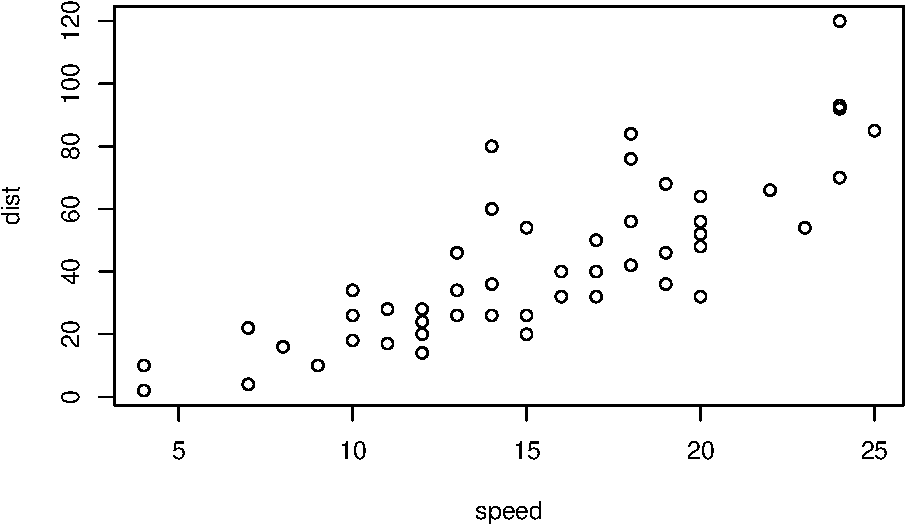
\includegraphics{01-intro_files/figure-latex/unnamed-chunk-1-1.pdf}

\begin{Shaded}
\begin{Highlighting}[]
\FunctionTok{plot}\NormalTok{(cars}\SpecialCharTok{$}\NormalTok{speed,cars}\SpecialCharTok{$}\NormalTok{dist) }\CommentTok{\#同上}
\end{Highlighting}
\end{Shaded}

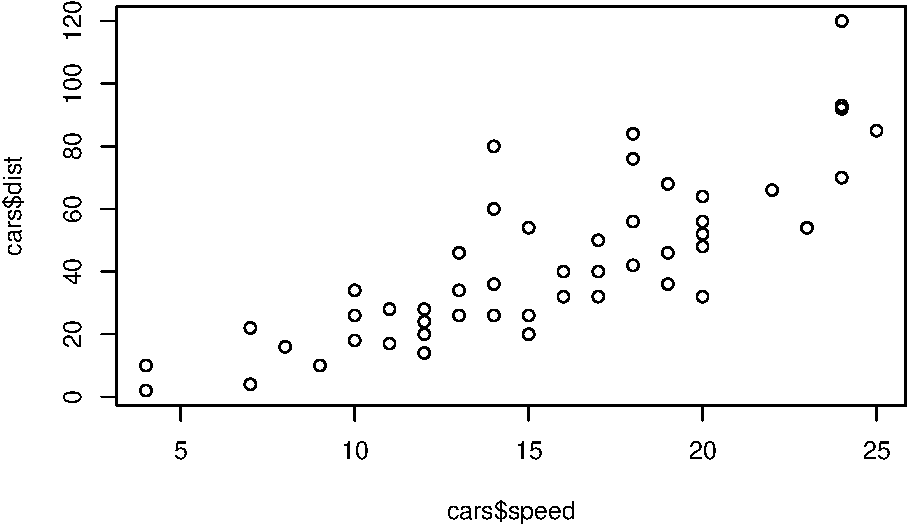
\includegraphics{01-intro_files/figure-latex/unnamed-chunk-1-2.pdf}

\begin{Shaded}
\begin{Highlighting}[]
\CommentTok{\#包括简单自变量为定量变量及定性变量的回归}

\FunctionTok{ncol}\NormalTok{(cars);}\FunctionTok{nrow}\NormalTok{(cars) }\CommentTok{\#cars的行列数}
\end{Highlighting}
\end{Shaded}

\begin{verbatim}
## [1] 2
\end{verbatim}

\begin{verbatim}
## [1] 50
\end{verbatim}

\begin{Shaded}
\begin{Highlighting}[]
\FunctionTok{dim}\NormalTok{(cars) }\CommentTok{\#cars的维数}
\end{Highlighting}
\end{Shaded}

\begin{verbatim}
## [1] 50  2
\end{verbatim}

\begin{Shaded}
\begin{Highlighting}[]
\FunctionTok{lm}\NormalTok{(dist }\SpecialCharTok{\textasciitilde{}}\NormalTok{ speed, }\AttributeTok{data =}\NormalTok{ cars)}\CommentTok{\#以dist为因变量,speed为自变量做OLS回归}
\end{Highlighting}
\end{Shaded}

\begin{verbatim}
## 
## Call:
## lm(formula = dist ~ speed, data = cars)
## 
## Coefficients:
## (Intercept)        speed  
##     -17.579        3.932
\end{verbatim}

\begin{Shaded}
\begin{Highlighting}[]
\NormalTok{cars}\SpecialCharTok{$}\NormalTok{qspeed }\OtherTok{=}\FunctionTok{cut}\NormalTok{(cars}\SpecialCharTok{$}\NormalTok{speed, }\AttributeTok{breaks=}\FunctionTok{quantile}\NormalTok{(cars}\SpecialCharTok{$}\NormalTok{speed),}
\AttributeTok{include.lowest =} \ConstantTok{TRUE}\NormalTok{) }\CommentTok{\#增加定性变量qspeed, 四分位点为分割点}
\FunctionTok{names}\NormalTok{(cars) }\CommentTok{\#数据cars多了一个变量}
\end{Highlighting}
\end{Shaded}

\begin{verbatim}
## [1] "speed"  "dist"   "qspeed"
\end{verbatim}

\begin{Shaded}
\begin{Highlighting}[]
\NormalTok{cars[}\DecValTok{3}\NormalTok{]}\CommentTok{\#第三个变量的值, 和cars[,3]类似}
\end{Highlighting}
\end{Shaded}

\begin{verbatim}
##     qspeed
## 1   [4,12]
## 2   [4,12]
## 3   [4,12]
## 4   [4,12]
## 5   [4,12]
## 6   [4,12]
## 7   [4,12]
## 8   [4,12]
## 9   [4,12]
## 10  [4,12]
## 11  [4,12]
## 12  [4,12]
## 13  [4,12]
## 14  [4,12]
## 15  [4,12]
## 16 (12,15]
## 17 (12,15]
## 18 (12,15]
## 19 (12,15]
## 20 (12,15]
## 21 (12,15]
## 22 (12,15]
## 23 (12,15]
## 24 (12,15]
## 25 (12,15]
## 26 (12,15]
## 27 (15,19]
## 28 (15,19]
## 29 (15,19]
## 30 (15,19]
## 31 (15,19]
## 32 (15,19]
## 33 (15,19]
## 34 (15,19]
## 35 (15,19]
## 36 (15,19]
## 37 (15,19]
## 38 (15,19]
## 39 (19,25]
## 40 (19,25]
## 41 (19,25]
## 42 (19,25]
## 43 (19,25]
## 44 (19,25]
## 45 (19,25]
## 46 (19,25]
## 47 (19,25]
## 48 (19,25]
## 49 (19,25]
## 50 (19,25]
\end{verbatim}

\begin{Shaded}
\begin{Highlighting}[]
\FunctionTok{table}\NormalTok{(cars[}\DecValTok{3}\NormalTok{])}\CommentTok{\#列表}
\end{Highlighting}
\end{Shaded}

\begin{verbatim}
## 
##  [4,12] (12,15] (15,19] (19,25] 
##      15      11      12      12
\end{verbatim}

\begin{Shaded}
\begin{Highlighting}[]
\FunctionTok{is.factor}\NormalTok{(cars}\SpecialCharTok{$}\NormalTok{qspeed)}
\end{Highlighting}
\end{Shaded}

\begin{verbatim}
## [1] TRUE
\end{verbatim}

\begin{Shaded}
\begin{Highlighting}[]
\FunctionTok{plot}\NormalTok{(dist }\SpecialCharTok{\textasciitilde{}}\NormalTok{ qspeed, }\AttributeTok{data =}\NormalTok{ cars)}\CommentTok{\#点出箱线图}
\end{Highlighting}
\end{Shaded}

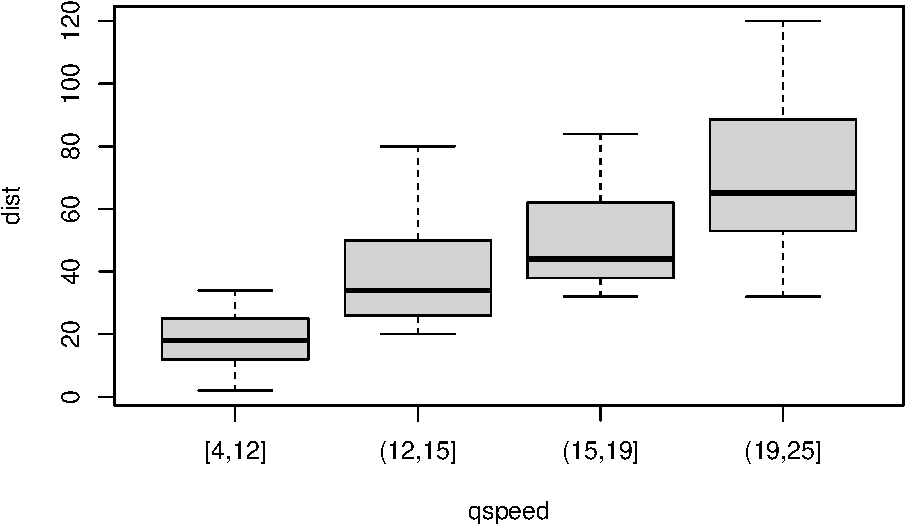
\includegraphics{01-intro_files/figure-latex/unnamed-chunk-1-3.pdf}

\begin{Shaded}
\begin{Highlighting}[]
\CommentTok{\#拟合线性模型(简单最小二乘回归):}
\NormalTok{(}\AttributeTok{a=}\FunctionTok{lm}\NormalTok{(dist }\SpecialCharTok{\textasciitilde{}}\NormalTok{ qspeed, }\AttributeTok{data =}\NormalTok{ cars))}
\end{Highlighting}
\end{Shaded}

\begin{verbatim}
## 
## Call:
## lm(formula = dist ~ qspeed, data = cars)
## 
## Coefficients:
##   (Intercept)  qspeed(12,15]  qspeed(15,19]  qspeed(19,25]  
##         18.20          21.98          31.97          51.13
\end{verbatim}

\begin{Shaded}
\begin{Highlighting}[]
\FunctionTok{summary}\NormalTok{(a)}\CommentTok{\#回归结果(包括一些检验)}
\end{Highlighting}
\end{Shaded}

\begin{verbatim}
## 
## Call:
## lm(formula = dist ~ qspeed, data = cars)
## 
## Residuals:
##    Min     1Q Median     3Q    Max 
## -37.33 -13.96  -3.75   9.30  50.67 
## 
## Coefficients:
##               Estimate Std. Error t value Pr(>|t|)    
## (Intercept)     18.200      4.551   3.999 0.000228 ***
## qspeed(12,15]   21.982      6.996   3.142 0.002933 ** 
## qspeed(15,19]   31.967      6.826   4.683 2.52e-05 ***
## qspeed(19,25]   51.133      6.826   7.491 1.68e-09 ***
## ---
## Signif. codes:  0 '***' 0.001 '**' 0.01 '*' 0.05 '.' 0.1 ' ' 1
## 
## Residual standard error: 17.62 on 46 degrees of freedom
## Multiple R-squared:  0.5609, Adjusted R-squared:  0.5322 
## F-statistic: 19.59 on 3 and 46 DF,  p-value: 2.517e-08
\end{verbatim}

\begin{Shaded}
\begin{Highlighting}[]
\NormalTok{x }\OtherTok{\textless{}{-}} \FunctionTok{round}\NormalTok{(}\FunctionTok{runif}\NormalTok{(}\DecValTok{20}\NormalTok{,}\DecValTok{0}\NormalTok{,}\DecValTok{20}\NormalTok{), }\AttributeTok{digits=}\DecValTok{2}\NormalTok{)}\CommentTok{\#四舍五入}
\FunctionTok{summary}\NormalTok{(x) }\CommentTok{\#汇总}
\end{Highlighting}
\end{Shaded}

\begin{verbatim}
##    Min. 1st Qu.  Median    Mean 3rd Qu.    Max. 
##    1.28    6.74   12.36   11.29   16.89   18.06
\end{verbatim}

\begin{Shaded}
\begin{Highlighting}[]
\FunctionTok{min}\NormalTok{(x);}\FunctionTok{max}\NormalTok{(x) }\CommentTok{\#极值, 与range(x)类似}
\end{Highlighting}
\end{Shaded}

\begin{verbatim}
## [1] 1.28
\end{verbatim}

\begin{verbatim}
## [1] 18.06
\end{verbatim}

\begin{Shaded}
\begin{Highlighting}[]
\FunctionTok{median}\NormalTok{(x)  }\CommentTok{\# 中位数(median)}
\end{Highlighting}
\end{Shaded}

\begin{verbatim}
## [1] 12.36
\end{verbatim}

\begin{Shaded}
\begin{Highlighting}[]
\FunctionTok{mean}\NormalTok{(x)    }\CommentTok{\# 均值(mean)}
\end{Highlighting}
\end{Shaded}

\begin{verbatim}
## [1] 11.29
\end{verbatim}

\begin{Shaded}
\begin{Highlighting}[]
\FunctionTok{var}\NormalTok{(x)     }\CommentTok{\#方差(variance)}
\end{Highlighting}
\end{Shaded}

\begin{verbatim}
## [1] 30.12734
\end{verbatim}

\begin{Shaded}
\begin{Highlighting}[]
\FunctionTok{sd}\NormalTok{(x)      }\CommentTok{\# 标准差(standard deviation),为方差的平方根}
\end{Highlighting}
\end{Shaded}

\begin{verbatim}
## [1] 5.488837
\end{verbatim}

\begin{Shaded}
\begin{Highlighting}[]
\FunctionTok{sqrt}\NormalTok{(}\FunctionTok{var}\NormalTok{(x)) }\CommentTok{\#平方根}
\end{Highlighting}
\end{Shaded}

\begin{verbatim}
## [1] 5.488837
\end{verbatim}

\begin{Shaded}
\begin{Highlighting}[]
\FunctionTok{rank}\NormalTok{(x)    }\CommentTok{\# 秩(rank)}
\end{Highlighting}
\end{Shaded}

\begin{verbatim}
##  [1]  1  5 13  6 11 15 16  8  7 19 12 14 10 20  4  3 18  9 17  2
\end{verbatim}

\begin{Shaded}
\begin{Highlighting}[]
\FunctionTok{order}\NormalTok{(x)}\CommentTok{\#升序排列的x的下标}
\end{Highlighting}
\end{Shaded}

\begin{verbatim}
##  [1]  1 20 16 15  2  4  9  8 18 13  5 11  3 12  6  7 19 17 10 14
\end{verbatim}

\begin{Shaded}
\begin{Highlighting}[]
\FunctionTok{order}\NormalTok{(x,}\AttributeTok{decreasing =}\NormalTok{ T)}\CommentTok{\#降序排列的x的下标}
\end{Highlighting}
\end{Shaded}

\begin{verbatim}
##  [1] 14 10 17 19  7  6 12  3 11  5 13 18  8  9  4  2 15 16 20  1
\end{verbatim}

\begin{Shaded}
\begin{Highlighting}[]
\NormalTok{x[}\FunctionTok{order}\NormalTok{(x)] }\CommentTok{\#和sort(x)相同}
\end{Highlighting}
\end{Shaded}

\begin{verbatim}
##  [1]  1.28  3.78  3.83  5.87  6.71  6.75  7.61  7.83 10.07 12.11 12.61 12.89
## [13] 14.47 14.82 16.81 17.12 17.54 17.73 17.91 18.06
\end{verbatim}

\begin{Shaded}
\begin{Highlighting}[]
\FunctionTok{sort}\NormalTok{(x)     }\CommentTok{\#同上: 升序排列的x}
\end{Highlighting}
\end{Shaded}

\begin{verbatim}
##  [1]  1.28  3.78  3.83  5.87  6.71  6.75  7.61  7.83 10.07 12.11 12.61 12.89
## [13] 14.47 14.82 16.81 17.12 17.54 17.73 17.91 18.06
\end{verbatim}

\begin{Shaded}
\begin{Highlighting}[]
\FunctionTok{sort}\NormalTok{(x,}\AttributeTok{decreasing=}\NormalTok{T)}\CommentTok{\#sort(x,dec=T) 降序排列的x}
\end{Highlighting}
\end{Shaded}

\begin{verbatim}
##  [1] 18.06 17.91 17.73 17.54 17.12 16.81 14.82 14.47 12.89 12.61 12.11 10.07
## [13]  7.83  7.61  6.75  6.71  5.87  3.83  3.78  1.28
\end{verbatim}

\begin{Shaded}
\begin{Highlighting}[]
\FunctionTok{sum}\NormalTok{(x);}\FunctionTok{length}\NormalTok{(x)}\CommentTok{\#元素和及向量元素个数}
\end{Highlighting}
\end{Shaded}

\begin{verbatim}
## [1] 225.8
\end{verbatim}

\begin{verbatim}
## [1] 20
\end{verbatim}

\begin{Shaded}
\begin{Highlighting}[]
\FunctionTok{round}\NormalTok{(x) }\CommentTok{\#四舍五入,等于round(x,0),而round(x,5)为留到小数点后5位}
\end{Highlighting}
\end{Shaded}

\begin{verbatim}
##  [1]  1  7 14  7 13 17 17  8  8 18 13 15 12 18  6  4 18 10 18  4
\end{verbatim}

\begin{Shaded}
\begin{Highlighting}[]
\FunctionTok{fivenum}\NormalTok{(x)  }\CommentTok{\# 五数汇总, quantile}
\end{Highlighting}
\end{Shaded}

\begin{verbatim}
## [1]  1.280  6.730 12.360 16.965 18.060
\end{verbatim}

\begin{Shaded}
\begin{Highlighting}[]
\FunctionTok{quantile}\NormalTok{(x) }\CommentTok{\# 分位点 quantile (different convention)有多种定义}
\end{Highlighting}
\end{Shaded}

\begin{verbatim}
##      0%     25%     50%     75%    100% 
##  1.2800  6.7400 12.3600 16.8875 18.0600
\end{verbatim}

\begin{Shaded}
\begin{Highlighting}[]
\FunctionTok{quantile}\NormalTok{(x, }\FunctionTok{c}\NormalTok{(}\DecValTok{0}\NormalTok{,.}\DecValTok{33}\NormalTok{,.}\DecValTok{66}\NormalTok{,}\DecValTok{1}\NormalTok{))}
\end{Highlighting}
\end{Shaded}

\begin{verbatim}
##      0%     33%     66%    100% 
##  1.2800  7.6694 14.6590 18.0600
\end{verbatim}

\begin{Shaded}
\begin{Highlighting}[]
\FunctionTok{mad}\NormalTok{(x) }\CommentTok{\# "median average distance":}
\end{Highlighting}
\end{Shaded}

\begin{verbatim}
## [1] 7.368522
\end{verbatim}

\begin{Shaded}
\begin{Highlighting}[]
\FunctionTok{cummax}\NormalTok{(x)}\CommentTok{\#累积最大值}
\end{Highlighting}
\end{Shaded}

\begin{verbatim}
##  [1]  1.28  6.71 14.47 14.47 14.47 16.81 17.12 17.12 17.12 17.91 17.91 17.91
## [13] 17.91 18.06 18.06 18.06 18.06 18.06 18.06 18.06
\end{verbatim}

\begin{Shaded}
\begin{Highlighting}[]
\FunctionTok{cummin}\NormalTok{(x)}\CommentTok{\#累积最小值}
\end{Highlighting}
\end{Shaded}

\begin{verbatim}
##  [1] 1.28 1.28 1.28 1.28 1.28 1.28 1.28 1.28 1.28 1.28 1.28 1.28 1.28 1.28 1.28
## [16] 1.28 1.28 1.28 1.28 1.28
\end{verbatim}

\begin{Shaded}
\begin{Highlighting}[]
\FunctionTok{cumprod}\NormalTok{(x)}\CommentTok{\#累积积}
\end{Highlighting}
\end{Shaded}

\begin{verbatim}
##  [1] 1.280000e+00 8.588800e+00 1.242799e+02 8.388896e+02 1.057840e+04
##  [6] 1.778229e+05 3.044327e+06 2.383708e+07 1.814002e+08 3.248878e+09
## [11] 4.187803e+10 6.206325e+11 7.515859e+12 1.357364e+14 7.967727e+14
## [16] 3.051640e+15 5.410557e+16 5.448431e+17 9.556548e+18 3.612375e+19
\end{verbatim}

\begin{Shaded}
\begin{Highlighting}[]
\FunctionTok{cor}\NormalTok{(x,}\FunctionTok{sin}\NormalTok{(x}\SpecialCharTok{/}\DecValTok{20}\NormalTok{)) }\CommentTok{\#线性相关系数 (linear correlation)}
\end{Highlighting}
\end{Shaded}

\begin{verbatim}
## [1] 0.9981333
\end{verbatim}

\begin{Shaded}
\begin{Highlighting}[]
\CommentTok{\#一些简单图形}
\NormalTok{x}\OtherTok{=}\FunctionTok{rnorm}\NormalTok{(}\DecValTok{200}\NormalTok{)}\CommentTok{\#将200个随机正态数赋值到x}
\FunctionTok{hist}\NormalTok{(x, }\AttributeTok{col =} \StringTok{"light blue"}\NormalTok{)}\CommentTok{\#直方图(histogram)}
\FunctionTok{rug}\NormalTok{(x) }\CommentTok{\#在直方图下面加上实际点的大小位置}
\end{Highlighting}
\end{Shaded}

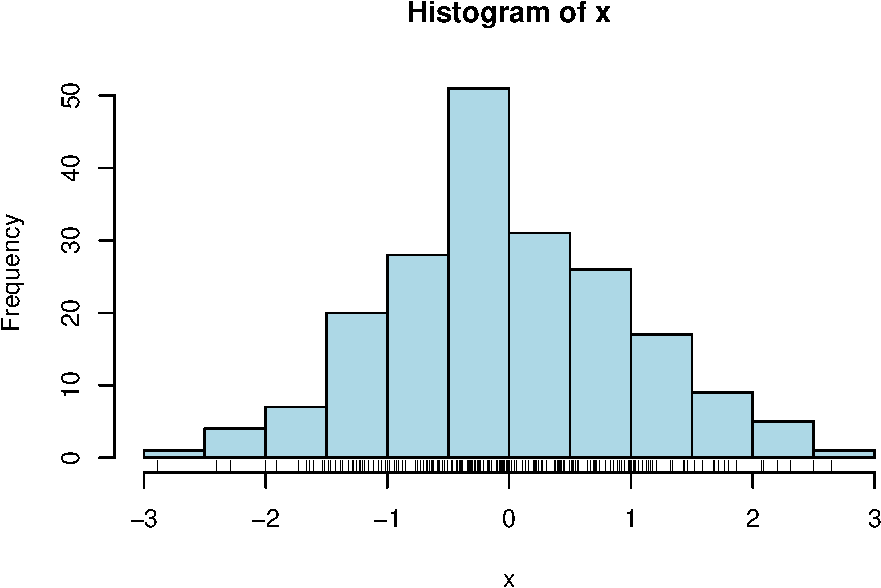
\includegraphics{01-intro_files/figure-latex/unnamed-chunk-1-4.pdf}

\begin{Shaded}
\begin{Highlighting}[]
\FunctionTok{stem}\NormalTok{(x)}\CommentTok{\#茎叶图}
\end{Highlighting}
\end{Shaded}

\begin{verbatim}
## 
##   The decimal point is at the |
## 
##   -2 | 9
##   -2 | 4330
##   -1 | 977665555
##   -1 | 4443333222222110000
##   -0 | 999999887777776666666665555555
##   -0 | 444444444333333333333333222222222211111111000000
##    0 | 0001112222222333444444444444
##    0 | 55555556666677777778899999
##    1 | 0000000011112223344
##    1 | 5566777889
##    2 | 1123
##    2 | 56
\end{verbatim}

\begin{Shaded}
\begin{Highlighting}[]
\NormalTok{x }\OtherTok{\textless{}{-}} \FunctionTok{rnorm}\NormalTok{(}\DecValTok{500}\NormalTok{)}
\NormalTok{y }\OtherTok{\textless{}{-}}\NormalTok{ x }\SpecialCharTok{+} \FunctionTok{rnorm}\NormalTok{(}\DecValTok{500}\NormalTok{) }\CommentTok{\#构造一个线性关系}
\FunctionTok{plot}\NormalTok{(y}\SpecialCharTok{\textasciitilde{}}\NormalTok{ x) }\CommentTok{\#散点图}
\NormalTok{a}\OtherTok{=}\FunctionTok{lm}\NormalTok{(y}\SpecialCharTok{\textasciitilde{}}\NormalTok{x) }\CommentTok{\#做回归}
\FunctionTok{abline}\NormalTok{(a,}\AttributeTok{col=}\StringTok{"red"}\NormalTok{)}\CommentTok{\#或者abline(lm(y\textasciitilde{}x),col="red")散点图加拟合线}
\end{Highlighting}
\end{Shaded}

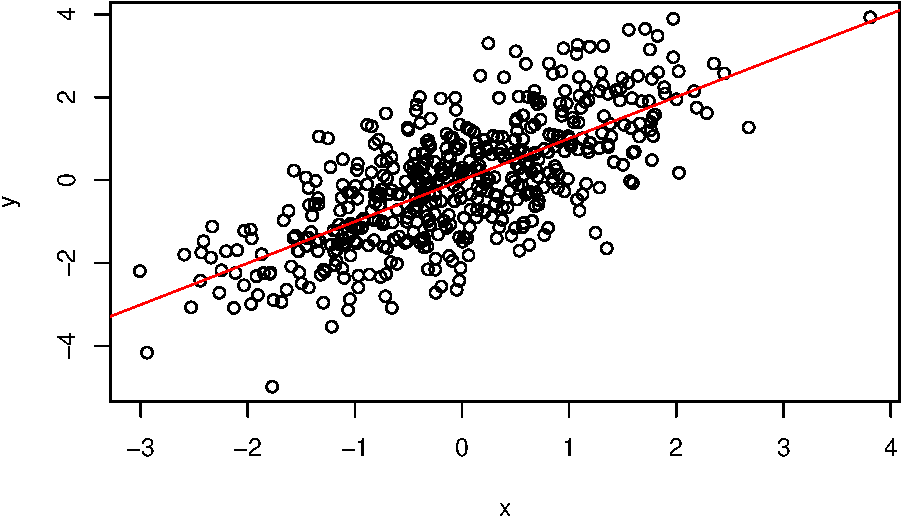
\includegraphics{01-intro_files/figure-latex/unnamed-chunk-1-5.pdf}

\begin{Shaded}
\begin{Highlighting}[]
\FunctionTok{print}\NormalTok{(}\StringTok{"Hello World!"}\NormalTok{)}
\end{Highlighting}
\end{Shaded}

\begin{verbatim}
## [1] "Hello World!"
\end{verbatim}

\begin{Shaded}
\begin{Highlighting}[]
\FunctionTok{paste}\NormalTok{(}\StringTok{"x 的最小值= "}\NormalTok{, }\FunctionTok{min}\NormalTok{(x)) }\CommentTok{\#打印}
\end{Highlighting}
\end{Shaded}

\begin{verbatim}
## [1] "x 的最小值=  -3.00804859892048"
\end{verbatim}

\begin{Shaded}
\begin{Highlighting}[]
\FunctionTok{demo}\NormalTok{(graphics)}\CommentTok{\#演示画图(点击Enter来切换)}
\end{Highlighting}
\end{Shaded}

\begin{verbatim}
## 
## 
##  demo(graphics)
##  ---- ~~~~~~~~
## 
## > #  Copyright (C) 1997-2009 The R Core Team
## > 
## > require(datasets)
## 
## > require(grDevices); require(graphics)
## 
## > ## Here is some code which illustrates some of the differences between
## > ## R and S graphics capabilities.  Note that colors are generally specified
## > ## by a character string name (taken from the X11 rgb.txt file) and that line
## > ## textures are given similarly.  The parameter "bg" sets the background
## > ## parameter for the plot and there is also an "fg" parameter which sets
## > ## the foreground color.
## > 
## > 
## > x <- stats::rnorm(50)
## 
## > opar <- par(bg = "white")
## 
## > plot(x, ann = FALSE, type = "n")
\end{verbatim}

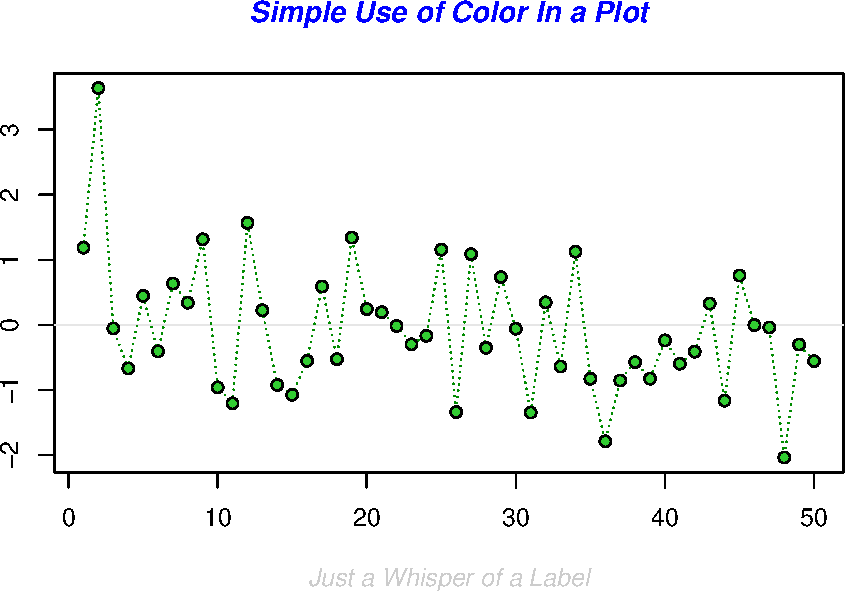
\includegraphics{01-intro_files/figure-latex/unnamed-chunk-1-6.pdf}

\begin{verbatim}
## 
## > abline(h = 0, col = gray(.90))
## 
## > lines(x, col = "green4", lty = "dotted")
## 
## > points(x, bg = "limegreen", pch = 21)
## 
## > title(main = "Simple Use of Color In a Plot",
## +       xlab = "Just a Whisper of a Label",
## +       col.main = "blue", col.lab = gray(.8),
## +       cex.main = 1.2, cex.lab = 1.0, font.main = 4, font.lab = 3)
## 
## > ## A little color wheel.    This code just plots equally spaced hues in
## > ## a pie chart.    If you have a cheap SVGA monitor (like me) you will
## > ## probably find that numerically equispaced does not mean visually
## > ## equispaced.  On my display at home, these colors tend to cluster at
## > ## the RGB primaries.  On the other hand on the SGI Indy at work the
## > ## effect is near perfect.
## > 
## > par(bg = "gray")
## 
## > pie(rep(1,24), col = rainbow(24), radius = 0.9)
\end{verbatim}

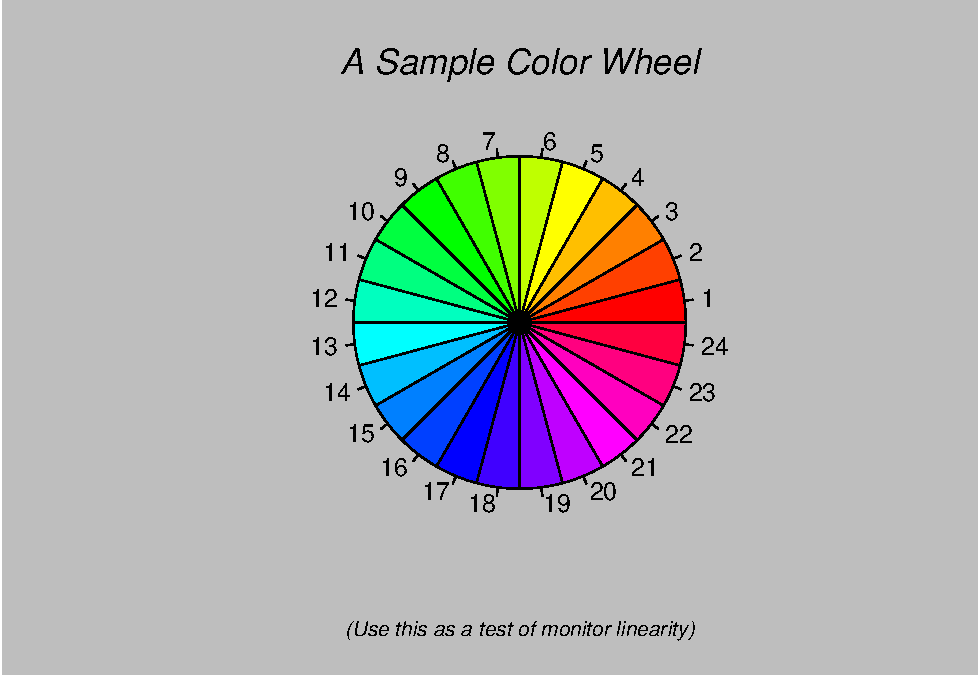
\includegraphics{01-intro_files/figure-latex/unnamed-chunk-1-7.pdf}

\begin{verbatim}
## 
## > title(main = "A Sample Color Wheel", cex.main = 1.4, font.main = 3)
## 
## > title(xlab = "(Use this as a test of monitor linearity)",
## +       cex.lab = 0.8, font.lab = 3)
## 
## > ## We have already confessed to having these.  This is just showing off X11
## > ## color names (and the example (from the postscript manual) is pretty "cute".
## > 
## > pie.sales <- c(0.12, 0.3, 0.26, 0.16, 0.04, 0.12)
## 
## > names(pie.sales) <- c("Blueberry", "Cherry",
## +              "Apple", "Boston Cream", "Other", "Vanilla Cream")
## 
## > pie(pie.sales,
## +     col = c("purple","violetred1","green3","cornsilk","cyan","white"))
\end{verbatim}

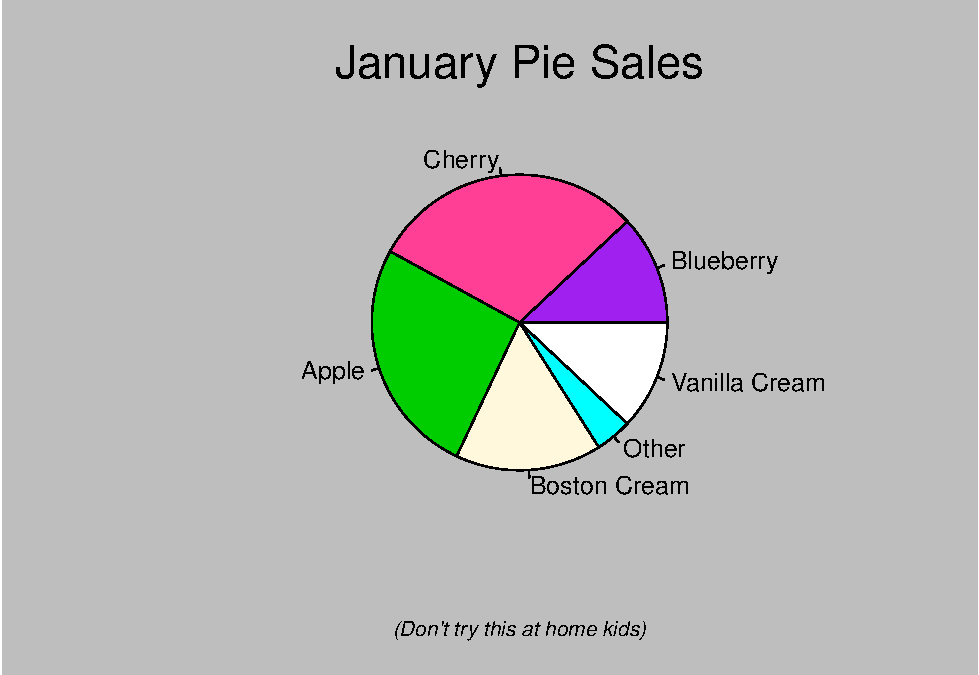
\includegraphics{01-intro_files/figure-latex/unnamed-chunk-1-8.pdf}

\begin{verbatim}
## 
## > title(main = "January Pie Sales", cex.main = 1.8, font.main = 1)
## 
## > title(xlab = "(Don't try this at home kids)", cex.lab = 0.8, font.lab = 3)
## 
## > ## Boxplots:  I couldn't resist the capability for filling the "box".
## > ## The use of color seems like a useful addition, it focuses attention
## > ## on the central bulk of the data.
## > 
## > par(bg="cornsilk")
## 
## > n <- 10
## 
## > g <- gl(n, 100, n*100)
## 
## > x <- rnorm(n*100) + sqrt(as.numeric(g))
## 
## > boxplot(split(x,g), col="lavender", notch=TRUE)
\end{verbatim}

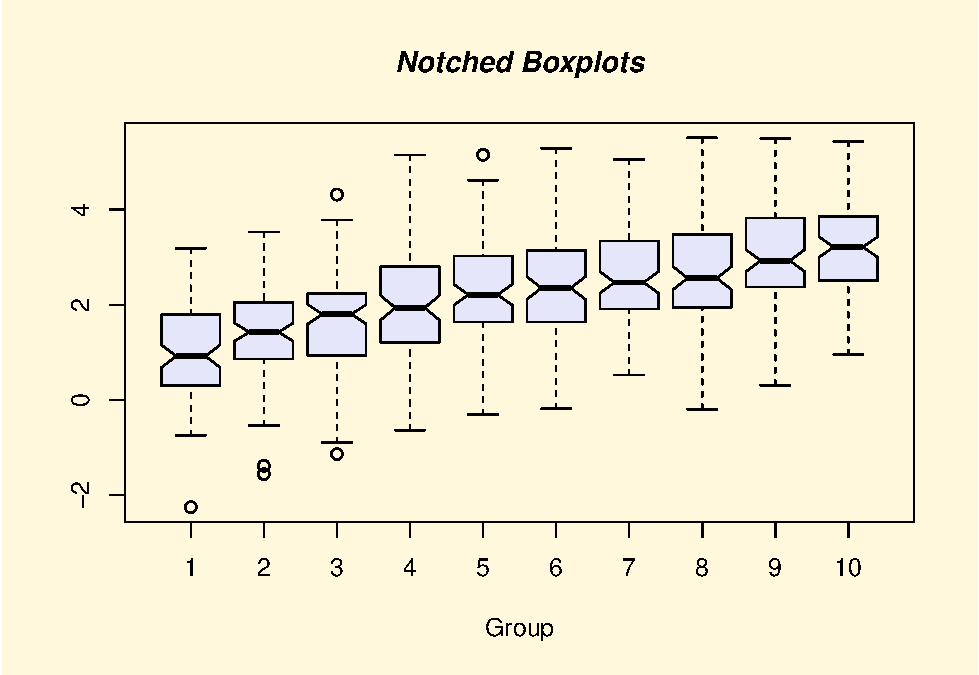
\includegraphics{01-intro_files/figure-latex/unnamed-chunk-1-9.pdf}

\begin{verbatim}
## 
## > title(main="Notched Boxplots", xlab="Group", font.main=4, font.lab=1)
## 
## > ## An example showing how to fill between curves.
## > 
## > par(bg="white")
## 
## > n <- 100
## 
## > x <- c(0,cumsum(rnorm(n)))
## 
## > y <- c(0,cumsum(rnorm(n)))
## 
## > xx <- c(0:n, n:0)
## 
## > yy <- c(x, rev(y))
## 
## > plot(xx, yy, type="n", xlab="Time", ylab="Distance")
\end{verbatim}

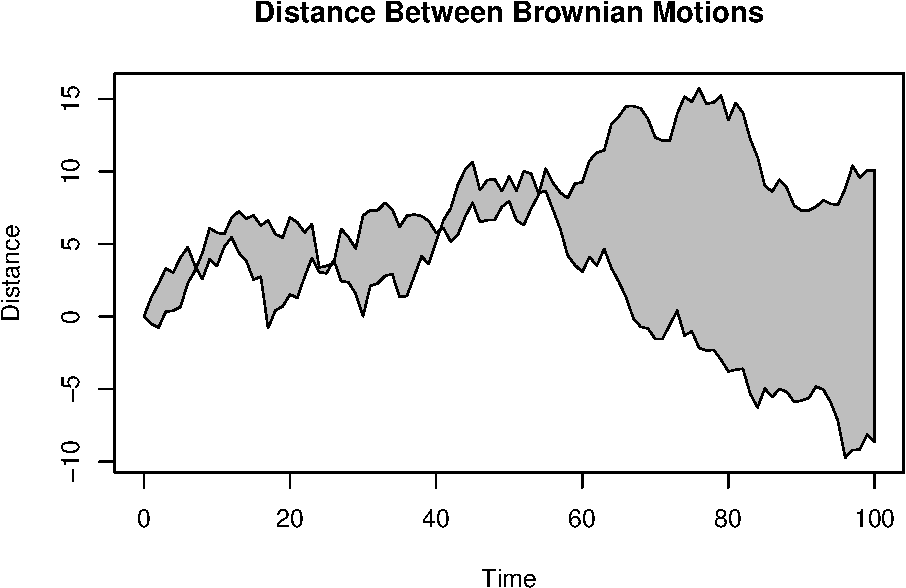
\includegraphics{01-intro_files/figure-latex/unnamed-chunk-1-10.pdf}

\begin{verbatim}
## 
## > polygon(xx, yy, col="gray")
## 
## > title("Distance Between Brownian Motions")
## 
## > ## Colored plot margins, axis labels and titles.    You do need to be
## > ## careful with these kinds of effects.    It's easy to go completely
## > ## over the top and you can end up with your lunch all over the keyboard.
## > ## On the other hand, my market research clients love it.
## > 
## > x <- c(0.00, 0.40, 0.86, 0.85, 0.69, 0.48, 0.54, 1.09, 1.11, 1.73, 2.05, 2.02)
## 
## > par(bg="lightgray")
## 
## > plot(x, type="n", axes=FALSE, ann=FALSE)
\end{verbatim}

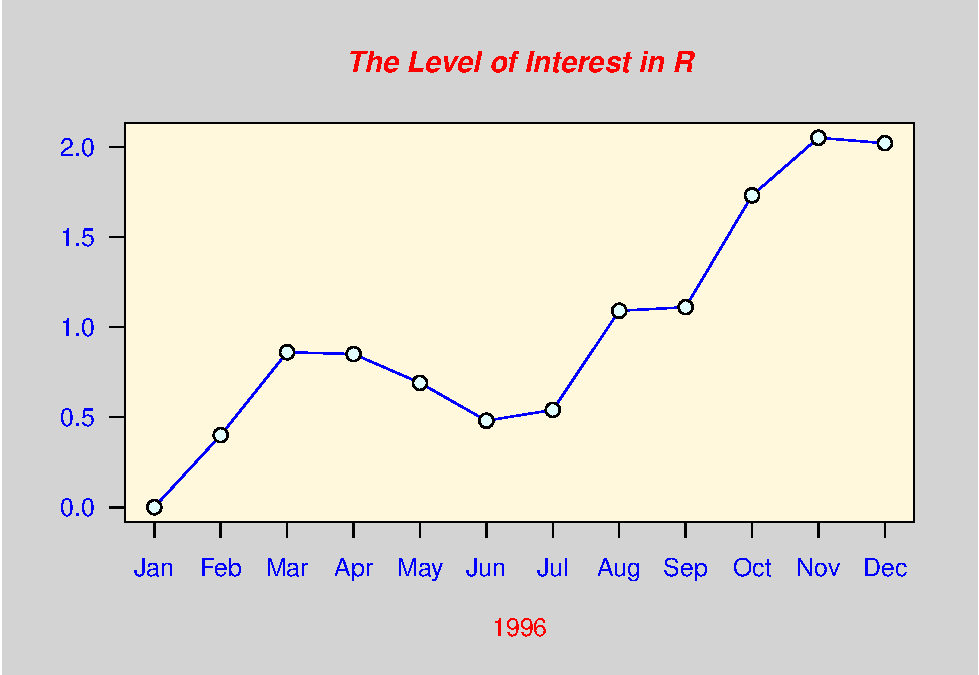
\includegraphics{01-intro_files/figure-latex/unnamed-chunk-1-11.pdf}

\begin{verbatim}
## 
## > usr <- par("usr")
## 
## > rect(usr[1], usr[3], usr[2], usr[4], col="cornsilk", border="black")
## 
## > lines(x, col="blue")
## 
## > points(x, pch=21, bg="lightcyan", cex=1.25)
## 
## > axis(2, col.axis="blue", las=1)
## 
## > axis(1, at=1:12, lab=month.abb, col.axis="blue")
## 
## > box()
## 
## > title(main= "The Level of Interest in R", font.main=4, col.main="red")
## 
## > title(xlab= "1996", col.lab="red")
## 
## > ## A filled histogram, showing how to change the font used for the
## > ## main title without changing the other annotation.
## > 
## > par(bg="cornsilk")
## 
## > x <- rnorm(1000)
## 
## > hist(x, xlim=range(-4, 4, x), col="lavender", main="")
\end{verbatim}

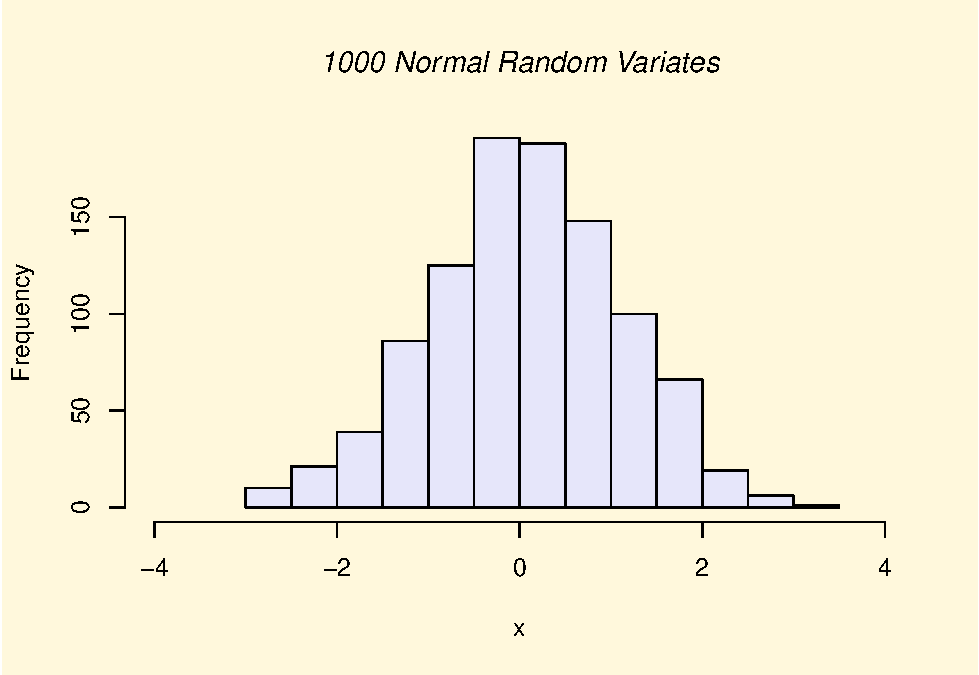
\includegraphics{01-intro_files/figure-latex/unnamed-chunk-1-12.pdf}

\begin{verbatim}
## 
## > title(main="1000 Normal Random Variates", font.main=3)
## 
## > ## A scatterplot matrix
## > ## The good old Iris data (yet again)
## > 
## > pairs(iris[1:4], main="Edgar Anderson's Iris Data", font.main=4, pch=19)
\end{verbatim}

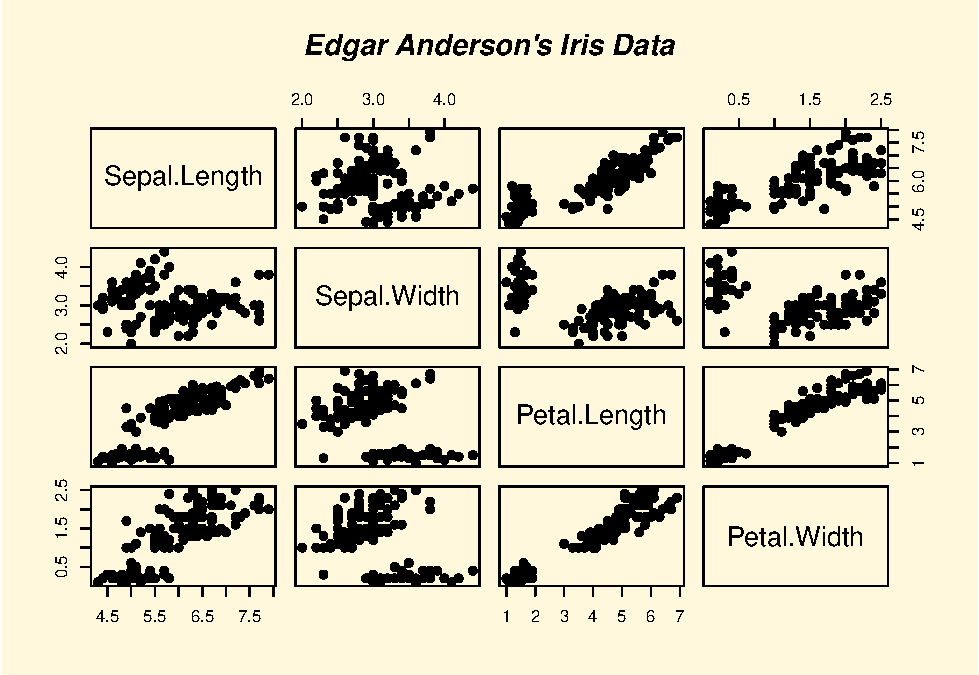
\includegraphics{01-intro_files/figure-latex/unnamed-chunk-1-13.pdf}

\begin{verbatim}
## 
## > pairs(iris[1:4], main="Edgar Anderson's Iris Data", pch=21,
## +       bg = c("red", "green3", "blue")[unclass(iris$Species)])
\end{verbatim}

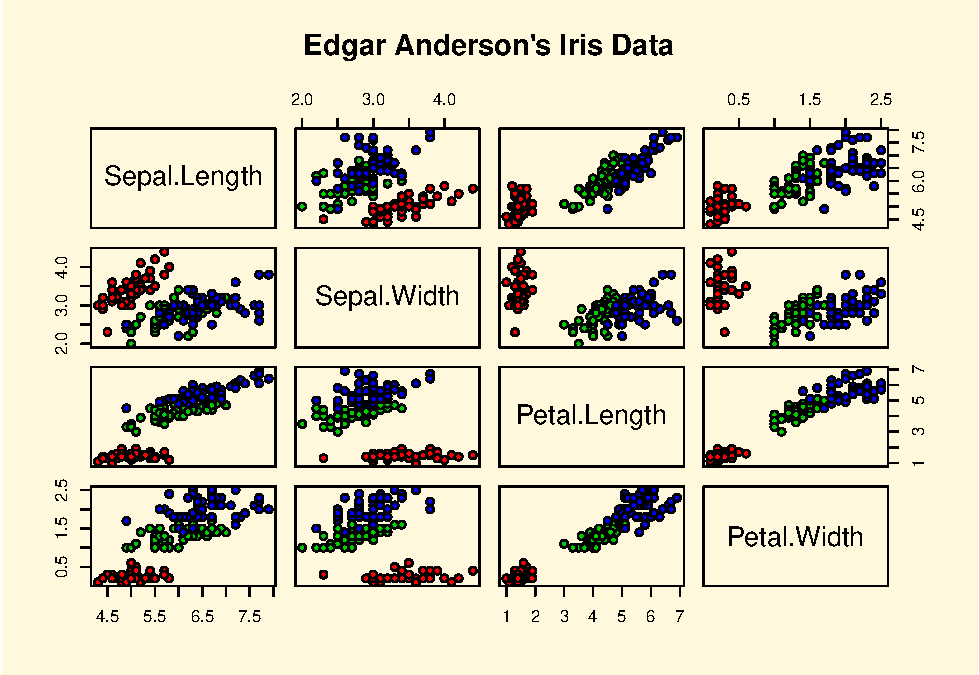
\includegraphics{01-intro_files/figure-latex/unnamed-chunk-1-14.pdf}

\begin{verbatim}
## 
## > ## Contour plotting
## > ## This produces a topographic map of one of Auckland's many volcanic "peaks".
## > 
## > x <- 10*1:nrow(volcano)
## 
## > y <- 10*1:ncol(volcano)
## 
## > lev <- pretty(range(volcano), 10)
## 
## > par(bg = "lightcyan")
## 
## > pin <- par("pin")
## 
## > xdelta <- diff(range(x))
## 
## > ydelta <- diff(range(y))
## 
## > xscale <- pin[1]/xdelta
## 
## > yscale <- pin[2]/ydelta
## 
## > scale <- min(xscale, yscale)
## 
## > xadd <- 0.5*(pin[1]/scale - xdelta)
## 
## > yadd <- 0.5*(pin[2]/scale - ydelta)
## 
## > plot(numeric(0), numeric(0),
## +      xlim = range(x)+c(-1,1)*xadd, ylim = range(y)+c(-1,1)*yadd,
## +      type = "n", ann = FALSE)
\end{verbatim}

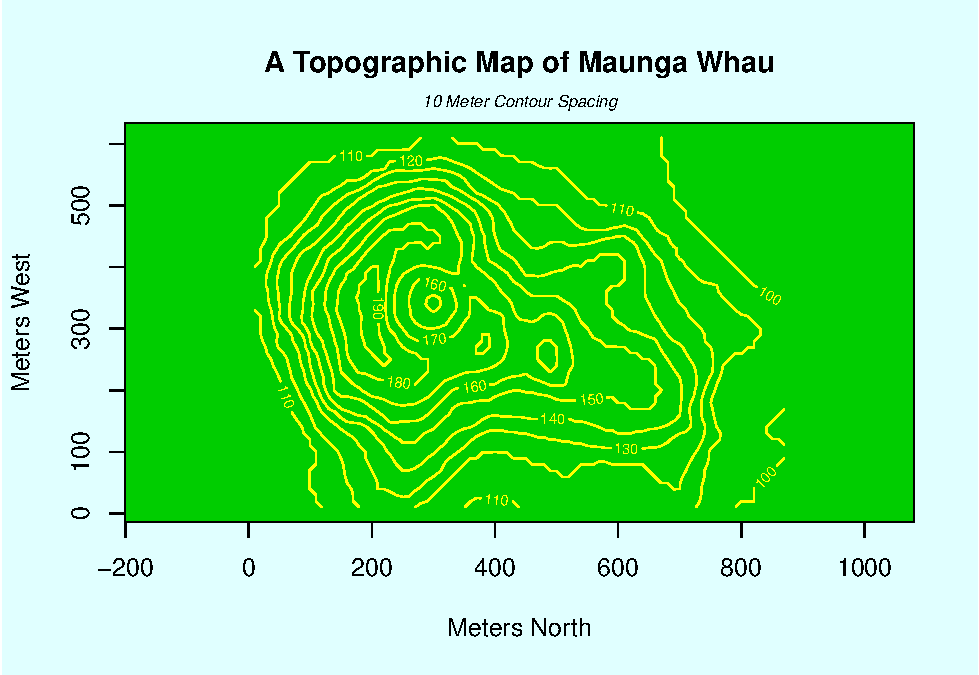
\includegraphics{01-intro_files/figure-latex/unnamed-chunk-1-15.pdf}

\begin{verbatim}
## 
## > usr <- par("usr")
## 
## > rect(usr[1], usr[3], usr[2], usr[4], col="green3")
## 
## > contour(x, y, volcano, levels = lev, col="yellow", lty="solid", add=TRUE)
## 
## > box()
## 
## > title("A Topographic Map of Maunga Whau", font= 4)
## 
## > title(xlab = "Meters North", ylab = "Meters West", font= 3)
## 
## > mtext("10 Meter Contour Spacing", side=3, line=0.35, outer=FALSE,
## +       at = mean(par("usr")[1:2]), cex=0.7, font=3)
## 
## > ## Conditioning plots
## > 
## > par(bg="cornsilk")
## 
## > coplot(lat ~ long | depth, data = quakes, pch = 21, bg = "green3")
\end{verbatim}

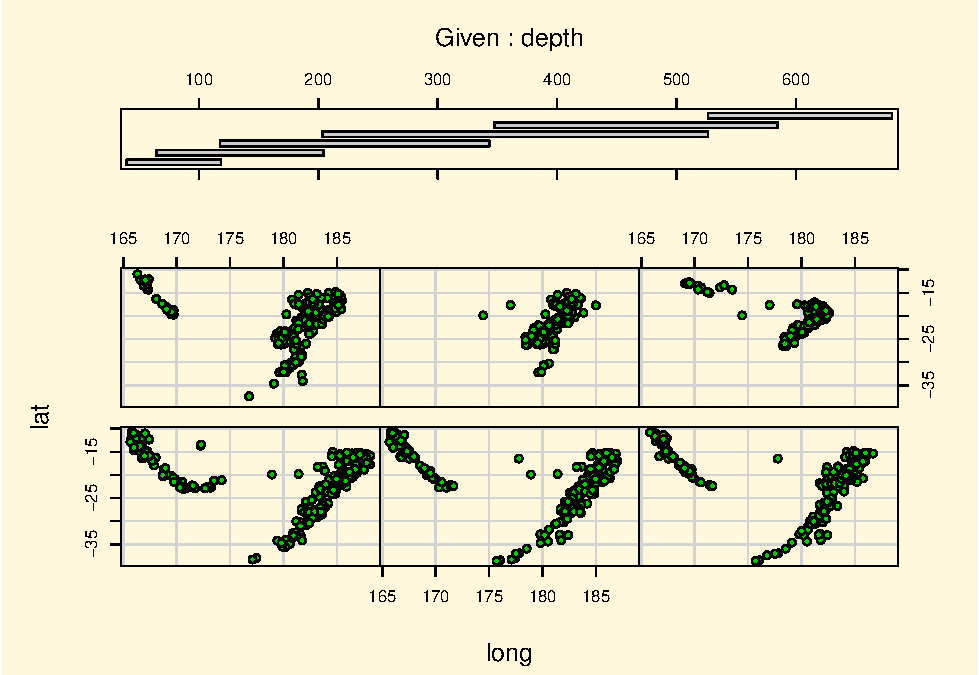
\includegraphics{01-intro_files/figure-latex/unnamed-chunk-1-16.pdf}

\begin{verbatim}
## 
## > par(opar)
\end{verbatim}

\begin{Shaded}
\begin{Highlighting}[]
\CommentTok{\#复数运算、求函数极值、多项式的根}
\NormalTok{(}\DecValTok{2}\SpecialCharTok{+}\NormalTok{4i)}\SpecialCharTok{\^{}{-}}\FloatTok{3.5}\SpecialCharTok{+}\NormalTok{(2i}\FloatTok{+4.5}\NormalTok{)}\SpecialCharTok{*}\NormalTok{(}\SpecialCharTok{{-}}\FloatTok{1.7{-}2.3}\NormalTok{i)}\SpecialCharTok{/}\NormalTok{((}\FloatTok{2.6}\SpecialCharTok{{-}}\NormalTok{7i)}\SpecialCharTok{*}\NormalTok{(}\SpecialCharTok{{-}}\DecValTok{4}\FloatTok{+5.1}\NormalTok{i))}\CommentTok{\#复数运算}
\end{Highlighting}
\end{Shaded}

\begin{verbatim}
## [1] -0.2790593-0.091246i
\end{verbatim}

\begin{Shaded}
\begin{Highlighting}[]
\CommentTok{\#下面构造一个10维复向量, 实部和虚部均为10个标准正态样本点:}
\NormalTok{(z }\OtherTok{\textless{}{-}}\FunctionTok{complex}\NormalTok{(}\AttributeTok{real=}\FunctionTok{rnorm}\NormalTok{(}\DecValTok{10}\NormalTok{), }\AttributeTok{imaginary =}\FunctionTok{rnorm}\NormalTok{(}\DecValTok{10}\NormalTok{)))}
\end{Highlighting}
\end{Shaded}

\begin{verbatim}
##  [1] -0.4742553+0.5064816i -0.0698126+0.5236044i -0.7625232+0.6249499i
##  [4] -0.5726097-2.9808548i -1.1276920+1.8869267i  0.1227265+0.4598803i
##  [7]  1.2287895+0.3914276i -0.5875730-1.1872535i -1.8391681+0.4443236i
## [10]  0.4978261-0.7539440i
\end{verbatim}

\begin{Shaded}
\begin{Highlighting}[]
\FunctionTok{complex}\NormalTok{(}\AttributeTok{re=}\FunctionTok{rnorm}\NormalTok{(}\DecValTok{3}\NormalTok{),}\AttributeTok{im=}\FunctionTok{rnorm}\NormalTok{(}\DecValTok{3}\NormalTok{))}\CommentTok{\#3维复向量}
\end{Highlighting}
\end{Shaded}

\begin{verbatim}
## [1]  0.2110114+0.6801056i -0.1367521-0.0557254i  0.0132440-0.4990980i
\end{verbatim}

\begin{Shaded}
\begin{Highlighting}[]
\FunctionTok{Re}\NormalTok{(z) }\CommentTok{\#实部}
\end{Highlighting}
\end{Shaded}

\begin{verbatim}
##  [1] -0.47425527 -0.06981258 -0.76252319 -0.57260970 -1.12769199  0.12272654
##  [7]  1.22878953 -0.58757302 -1.83916811  0.49782614
\end{verbatim}

\begin{Shaded}
\begin{Highlighting}[]
\FunctionTok{Im}\NormalTok{(z) }\CommentTok{\#虚部}
\end{Highlighting}
\end{Shaded}

\begin{verbatim}
##  [1]  0.5064816  0.5236044  0.6249499 -2.9808548  1.8869267  0.4598803
##  [7]  0.3914276 -1.1872535  0.4443236 -0.7539440
\end{verbatim}

\begin{Shaded}
\begin{Highlighting}[]
\FunctionTok{Mod}\NormalTok{(z) }\CommentTok{\#模}
\end{Highlighting}
\end{Shaded}

\begin{verbatim}
##  [1] 0.6938600 0.5282380 0.9859026 3.0353545 2.1982224 0.4759744 1.2896276
##  [8] 1.3246935 1.8920790 0.9034724
\end{verbatim}

\begin{Shaded}
\begin{Highlighting}[]
\FunctionTok{Arg}\NormalTok{(z) }\CommentTok{\#辐角}
\end{Highlighting}
\end{Shaded}

\begin{verbatim}
##  [1]  2.3233470  1.7033453  2.4550253 -1.7605803  2.1094745  1.3100076
##  [7]  0.3083847 -2.0303565  2.9045454 -0.9872172
\end{verbatim}

\begin{Shaded}
\begin{Highlighting}[]
\FunctionTok{choose}\NormalTok{(}\DecValTok{3}\NormalTok{,}\DecValTok{2}\NormalTok{) }\CommentTok{\#组合}
\end{Highlighting}
\end{Shaded}

\begin{verbatim}
## [1] 3
\end{verbatim}

\begin{Shaded}
\begin{Highlighting}[]
\FunctionTok{factorial}\NormalTok{(}\DecValTok{6}\NormalTok{)}\CommentTok{\#排列6!}
\end{Highlighting}
\end{Shaded}

\begin{verbatim}
## [1] 720
\end{verbatim}

\begin{Shaded}
\begin{Highlighting}[]
\CommentTok{\#求函数极值}
\NormalTok{f}\OtherTok{=}\ControlFlowTok{function}\NormalTok{(x) x}\SpecialCharTok{\^{}}\DecValTok{2}\SpecialCharTok{+}\DecValTok{2}\SpecialCharTok{*}\NormalTok{x}\SpecialCharTok{+}\DecValTok{1} \CommentTok{\#定义一个二次函数}
\FunctionTok{optimize}\NormalTok{(f,}\FunctionTok{c}\NormalTok{(}\SpecialCharTok{{-}}\DecValTok{2}\NormalTok{,}\DecValTok{2}\NormalTok{))}\CommentTok{\#在区间({-}2,2)内求极值}
\end{Highlighting}
\end{Shaded}

\begin{verbatim}
## $minimum
## [1] -1
## 
## $objective
## [1] 0
\end{verbatim}

\begin{Shaded}
\begin{Highlighting}[]
\FunctionTok{curve}\NormalTok{(f, }\AttributeTok{from =} \SpecialCharTok{{-}}\DecValTok{3}\NormalTok{,}\AttributeTok{to=}\DecValTok{2}\NormalTok{)}\CommentTok{\#在区间({-}3,2)内画上面定义的函数f图}
\end{Highlighting}
\end{Shaded}

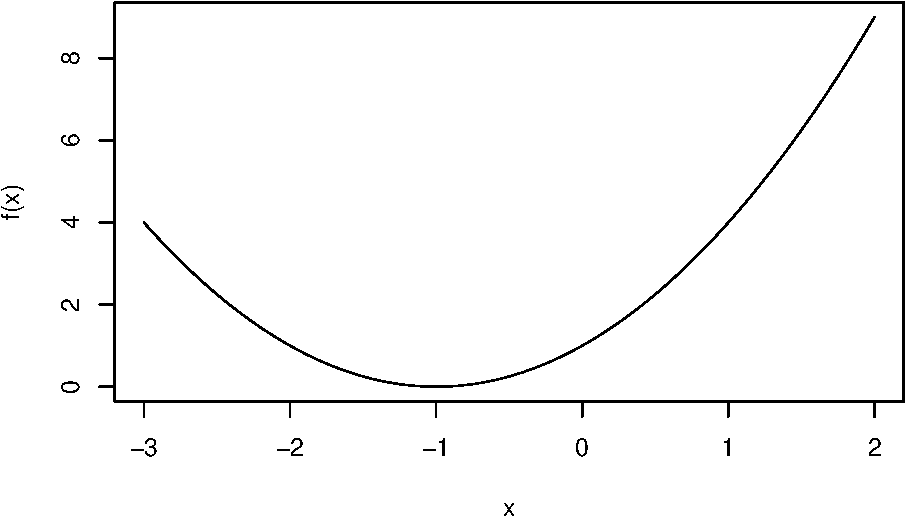
\includegraphics{01-intro_files/figure-latex/unnamed-chunk-1-17.pdf}

\begin{Shaded}
\begin{Highlighting}[]
\CommentTok{\#求从常数项开始到5次方项的系数分别为1, 2, 2, 4, {-}9, 8的多项式的根: }
\FunctionTok{polyroot}\NormalTok{(}\FunctionTok{c}\NormalTok{(}\DecValTok{1}\NormalTok{,}\DecValTok{2}\NormalTok{,}\DecValTok{2}\NormalTok{,}\DecValTok{4}\NormalTok{,}\SpecialCharTok{{-}}\DecValTok{9}\NormalTok{,}\DecValTok{8}\NormalTok{))}
\end{Highlighting}
\end{Shaded}

\begin{verbatim}
## [1] -0.1128081+0.4980033i -0.3912226+0.0000000i -0.1128081-0.4980033i
## [4]  0.8709194-0.6833257i  0.8709194+0.6833257i
\end{verbatim}

\begin{Shaded}
\begin{Highlighting}[]
\CommentTok{\#字符型向量和因子型变量}
\NormalTok{a}\OtherTok{=}\FunctionTok{factor}\NormalTok{(letters[}\DecValTok{1}\SpecialCharTok{:}\DecValTok{10}\NormalTok{]);a }\CommentTok{\#letters:小写字母向量,LETTERS:大写}
\end{Highlighting}
\end{Shaded}

\begin{verbatim}
##  [1] a b c d e f g h i j
## Levels: a b c d e f g h i j
\end{verbatim}

\begin{Shaded}
\begin{Highlighting}[]
\NormalTok{a[}\DecValTok{3}\NormalTok{]}\OtherTok{=}\StringTok{"w"} \CommentTok{\#不行! 会给出警告}
\end{Highlighting}
\end{Shaded}

\begin{verbatim}
## Warning in `[<-.factor`(`*tmp*`, 3, value = "w"): invalid factor level, NA
## generated
\end{verbatim}

\begin{Shaded}
\begin{Highlighting}[]
\NormalTok{a}\OtherTok{=}\FunctionTok{as.character}\NormalTok{(a) }\CommentTok{\#转换一下}
\NormalTok{a[}\DecValTok{3}\NormalTok{]}\OtherTok{=}\StringTok{"w"} \CommentTok{\#可以了}
\NormalTok{a;}\FunctionTok{factor}\NormalTok{(a) }\CommentTok{\#两种不同的类型}
\end{Highlighting}
\end{Shaded}

\begin{verbatim}
##  [1] "a" "b" "w" "d" "e" "f" "g" "h" "i" "j"
\end{verbatim}

\begin{verbatim}
##  [1] a b w d e f g h i j
## Levels: a b d e f g h i j w
\end{verbatim}

\begin{Shaded}
\begin{Highlighting}[]
\CommentTok{\#定性变量的水平:}
\FunctionTok{levels}\NormalTok{(}\FunctionTok{factor}\NormalTok{(a))}
\end{Highlighting}
\end{Shaded}

\begin{verbatim}
##  [1] "a" "b" "d" "e" "f" "g" "h" "i" "j" "w"
\end{verbatim}

\begin{Shaded}
\begin{Highlighting}[]
\NormalTok{sex}\OtherTok{=}\FunctionTok{sample}\NormalTok{(}\DecValTok{0}\SpecialCharTok{:}\DecValTok{1}\NormalTok{,}\DecValTok{10}\NormalTok{,}\AttributeTok{r=}\NormalTok{T)}
\NormalTok{sex}\OtherTok{=}\FunctionTok{factor}\NormalTok{(sex);}\FunctionTok{levels}\NormalTok{(sex)}
\end{Highlighting}
\end{Shaded}

\begin{verbatim}
## [1] "0" "1"
\end{verbatim}

\begin{Shaded}
\begin{Highlighting}[]
\CommentTok{\#改变因子的水平:}
\FunctionTok{levels}\NormalTok{(sex)}\OtherTok{=}\FunctionTok{c}\NormalTok{(}\StringTok{"Male"}\NormalTok{,}\StringTok{"Female"}\NormalTok{);}\FunctionTok{levels}\NormalTok{(sex)}
\end{Highlighting}
\end{Shaded}

\begin{verbatim}
## [1] "Male"   "Female"
\end{verbatim}

\begin{Shaded}
\begin{Highlighting}[]
\CommentTok{\#确定水平次序:}
\NormalTok{sex}\OtherTok{=}\FunctionTok{ordered}\NormalTok{(sex,}\FunctionTok{c}\NormalTok{(}\StringTok{"Female"}\NormalTok{,}\StringTok{"Male"}\NormalTok{));sex}
\end{Highlighting}
\end{Shaded}

\begin{verbatim}
##  [1] Female Female Female Female Male   Male   Male   Female Female Female
## Levels: Female < Male
\end{verbatim}

\begin{Shaded}
\begin{Highlighting}[]
\FunctionTok{levels}\NormalTok{(sex)}
\end{Highlighting}
\end{Shaded}

\begin{verbatim}
## [1] "Female" "Male"
\end{verbatim}

\begin{Shaded}
\begin{Highlighting}[]
\CommentTok{\#序列}

\NormalTok{(}\AttributeTok{z=}\FunctionTok{seq}\NormalTok{(}\SpecialCharTok{{-}}\DecValTok{1}\NormalTok{,}\DecValTok{10}\NormalTok{,}\AttributeTok{length=}\DecValTok{100}\NormalTok{))}\CommentTok{\#从{-}1到10等间隔的100个数组成的序列}
\end{Highlighting}
\end{Shaded}

\begin{verbatim}
##   [1] -1.0000000 -0.8888889 -0.7777778 -0.6666667 -0.5555556 -0.4444444
##   [7] -0.3333333 -0.2222222 -0.1111111  0.0000000  0.1111111  0.2222222
##  [13]  0.3333333  0.4444444  0.5555556  0.6666667  0.7777778  0.8888889
##  [19]  1.0000000  1.1111111  1.2222222  1.3333333  1.4444444  1.5555556
##  [25]  1.6666667  1.7777778  1.8888889  2.0000000  2.1111111  2.2222222
##  [31]  2.3333333  2.4444444  2.5555556  2.6666667  2.7777778  2.8888889
##  [37]  3.0000000  3.1111111  3.2222222  3.3333333  3.4444444  3.5555556
##  [43]  3.6666667  3.7777778  3.8888889  4.0000000  4.1111111  4.2222222
##  [49]  4.3333333  4.4444444  4.5555556  4.6666667  4.7777778  4.8888889
##  [55]  5.0000000  5.1111111  5.2222222  5.3333333  5.4444444  5.5555556
##  [61]  5.6666667  5.7777778  5.8888889  6.0000000  6.1111111  6.2222222
##  [67]  6.3333333  6.4444444  6.5555556  6.6666667  6.7777778  6.8888889
##  [73]  7.0000000  7.1111111  7.2222222  7.3333333  7.4444444  7.5555556
##  [79]  7.6666667  7.7777778  7.8888889  8.0000000  8.1111111  8.2222222
##  [85]  8.3333333  8.4444444  8.5555556  8.6666667  8.7777778  8.8888889
##  [91]  9.0000000  9.1111111  9.2222222  9.3333333  9.4444444  9.5555556
##  [97]  9.6666667  9.7777778  9.8888889 10.0000000
\end{verbatim}

\begin{Shaded}
\begin{Highlighting}[]
\NormalTok{z}\OtherTok{=}\FunctionTok{seq}\NormalTok{(}\SpecialCharTok{{-}}\DecValTok{1}\NormalTok{,}\DecValTok{10}\NormalTok{,}\AttributeTok{len=}\DecValTok{100}\NormalTok{)}\CommentTok{\#和上面写法等价}
\NormalTok{(}\AttributeTok{z=}\FunctionTok{seq}\NormalTok{(}\DecValTok{10}\NormalTok{,}\SpecialCharTok{{-}}\DecValTok{1}\NormalTok{,}\SpecialCharTok{{-}}\FloatTok{0.1}\NormalTok{)) }\CommentTok{\#10到{-}1间隔为{-}0.1的序列}
\end{Highlighting}
\end{Shaded}

\begin{verbatim}
##   [1] 10.0  9.9  9.8  9.7  9.6  9.5  9.4  9.3  9.2  9.1  9.0  8.9  8.8  8.7  8.6
##  [16]  8.5  8.4  8.3  8.2  8.1  8.0  7.9  7.8  7.7  7.6  7.5  7.4  7.3  7.2  7.1
##  [31]  7.0  6.9  6.8  6.7  6.6  6.5  6.4  6.3  6.2  6.1  6.0  5.9  5.8  5.7  5.6
##  [46]  5.5  5.4  5.3  5.2  5.1  5.0  4.9  4.8  4.7  4.6  4.5  4.4  4.3  4.2  4.1
##  [61]  4.0  3.9  3.8  3.7  3.6  3.5  3.4  3.3  3.2  3.1  3.0  2.9  2.8  2.7  2.6
##  [76]  2.5  2.4  2.3  2.2  2.1  2.0  1.9  1.8  1.7  1.6  1.5  1.4  1.3  1.2  1.1
##  [91]  1.0  0.9  0.8  0.7  0.6  0.5  0.4  0.3  0.2  0.1  0.0 -0.1 -0.2 -0.3 -0.4
## [106] -0.5 -0.6 -0.7 -0.8 -0.9 -1.0
\end{verbatim}

\begin{Shaded}
\begin{Highlighting}[]
\NormalTok{(}\AttributeTok{x=}\FunctionTok{rep}\NormalTok{(}\DecValTok{1}\SpecialCharTok{:}\DecValTok{3}\NormalTok{,}\DecValTok{3}\NormalTok{))  }\CommentTok{\#三次重复1:3}
\end{Highlighting}
\end{Shaded}

\begin{verbatim}
## [1] 1 2 3 1 2 3 1 2 3
\end{verbatim}

\begin{Shaded}
\begin{Highlighting}[]
\NormalTok{(}\AttributeTok{x=}\FunctionTok{rep}\NormalTok{(}\DecValTok{3}\SpecialCharTok{:}\DecValTok{5}\NormalTok{,}\DecValTok{1}\SpecialCharTok{:}\DecValTok{3}\NormalTok{)) }\CommentTok{\#自己看, 这又是什么呢?}
\end{Highlighting}
\end{Shaded}

\begin{verbatim}
## [1] 3 4 4 5 5 5
\end{verbatim}

\begin{Shaded}
\begin{Highlighting}[]
\NormalTok{x}\OtherTok{=}\FunctionTok{rep}\NormalTok{(}\FunctionTok{c}\NormalTok{(}\DecValTok{1}\NormalTok{,}\DecValTok{10}\NormalTok{),}\FunctionTok{c}\NormalTok{(}\DecValTok{4}\NormalTok{,}\DecValTok{5}\NormalTok{))}
\NormalTok{w}\OtherTok{=}\FunctionTok{c}\NormalTok{(}\DecValTok{1}\NormalTok{,}\DecValTok{3}\NormalTok{,x,z);w[}\DecValTok{3}\NormalTok{]}\CommentTok{\#把数据(包括向量)组合(combine)成一个向量}
\end{Highlighting}
\end{Shaded}

\begin{verbatim}
## [1] 1
\end{verbatim}

\begin{Shaded}
\begin{Highlighting}[]
\NormalTok{x}\OtherTok{=}\FunctionTok{rep}\NormalTok{(}\DecValTok{0}\NormalTok{,}\DecValTok{10}\NormalTok{);z}\OtherTok{=}\DecValTok{1}\SpecialCharTok{:}\DecValTok{3}\NormalTok{;x}\SpecialCharTok{+}\NormalTok{z }\CommentTok{\#向量加法(如果长度不同, R给出警告和结果)}
\end{Highlighting}
\end{Shaded}

\begin{verbatim}
## Warning in x + z: longer object length is not a multiple of shorter object
## length
\end{verbatim}

\begin{verbatim}
##  [1] 1 2 3 1 2 3 1 2 3 1
\end{verbatim}

\begin{Shaded}
\begin{Highlighting}[]
\NormalTok{x}\SpecialCharTok{*}\NormalTok{z   }\CommentTok{\#向量乘法}
\end{Highlighting}
\end{Shaded}

\begin{verbatim}
## Warning in x * z: longer object length is not a multiple of shorter object
## length
\end{verbatim}

\begin{verbatim}
##  [1] 0 0 0 0 0 0 0 0 0 0
\end{verbatim}

\begin{Shaded}
\begin{Highlighting}[]
\FunctionTok{rev}\NormalTok{(x)}\CommentTok{\#颠倒次序}
\end{Highlighting}
\end{Shaded}

\begin{verbatim}
##  [1] 0 0 0 0 0 0 0 0 0 0
\end{verbatim}

\begin{Shaded}
\begin{Highlighting}[]
\NormalTok{z}\OtherTok{=}\FunctionTok{c}\NormalTok{(}\StringTok{"no cat"}\NormalTok{,}\StringTok{"has "}\NormalTok{,}\StringTok{"nine"}\NormalTok{,}\StringTok{"tails"}\NormalTok{) }\CommentTok{\#字符向量}
\NormalTok{z[}\DecValTok{1}\NormalTok{]}\SpecialCharTok{==}\StringTok{"no cat"} \CommentTok{\#双等号为逻辑等式}
\end{Highlighting}
\end{Shaded}

\begin{verbatim}
## [1] TRUE
\end{verbatim}

\begin{Shaded}
\begin{Highlighting}[]
\NormalTok{z}\OtherTok{=}\DecValTok{1}\SpecialCharTok{:}\DecValTok{5}
\NormalTok{z[}\DecValTok{7}\NormalTok{]}\OtherTok{=}\DecValTok{8}\NormalTok{;z }\CommentTok{\#什么结果? 注:NA为缺失值(not available)}
\end{Highlighting}
\end{Shaded}

\begin{verbatim}
## [1]  1  2  3  4  5 NA  8
\end{verbatim}

\begin{Shaded}
\begin{Highlighting}[]
\NormalTok{z}\OtherTok{=}\ConstantTok{NULL}
\NormalTok{z[}\FunctionTok{c}\NormalTok{(}\DecValTok{1}\NormalTok{,}\DecValTok{3}\NormalTok{,}\DecValTok{5}\NormalTok{)]}\OtherTok{=}\DecValTok{1}\SpecialCharTok{:}\DecValTok{3}\NormalTok{;}
\NormalTok{z}
\end{Highlighting}
\end{Shaded}

\begin{verbatim}
## [1]  1 NA  2 NA  3
\end{verbatim}

\begin{Shaded}
\begin{Highlighting}[]
\FunctionTok{rnorm}\NormalTok{(}\DecValTok{10}\NormalTok{)[}\FunctionTok{c}\NormalTok{(}\DecValTok{2}\NormalTok{,}\DecValTok{5}\NormalTok{)]}
\end{Highlighting}
\end{Shaded}

\begin{verbatim}
## [1]  0.4232452 -1.2447383
\end{verbatim}

\begin{Shaded}
\begin{Highlighting}[]
\NormalTok{z[}\SpecialCharTok{{-}}\FunctionTok{c}\NormalTok{(}\DecValTok{1}\NormalTok{,}\DecValTok{3}\NormalTok{)]}\CommentTok{\#去掉第1、3元素}
\end{Highlighting}
\end{Shaded}

\begin{verbatim}
## [1] NA NA  3
\end{verbatim}

\begin{Shaded}
\begin{Highlighting}[]
\NormalTok{z}\OtherTok{=}\FunctionTok{sample}\NormalTok{(}\DecValTok{1}\SpecialCharTok{:}\DecValTok{100}\NormalTok{,}\DecValTok{10}\NormalTok{);z}
\end{Highlighting}
\end{Shaded}

\begin{verbatim}
##  [1] 57 59 72 81 35 80 78 46  9 50
\end{verbatim}

\begin{Shaded}
\begin{Highlighting}[]
\FunctionTok{which}\NormalTok{(z}\SpecialCharTok{==}\FunctionTok{max}\NormalTok{(z))}\CommentTok{\#给出最大值的下标}
\end{Highlighting}
\end{Shaded}

\begin{verbatim}
## [1] 4
\end{verbatim}

\begin{Shaded}
\begin{Highlighting}[]
\CommentTok{\#矩阵}
\NormalTok{x}\OtherTok{=}\FunctionTok{sample}\NormalTok{(}\DecValTok{1}\SpecialCharTok{:}\DecValTok{100}\NormalTok{,}\DecValTok{12}\NormalTok{);x }\CommentTok{\#抽样}
\end{Highlighting}
\end{Shaded}

\begin{verbatim}
##  [1] 74 77 82 90 35 53 73 32  9 97 25 87
\end{verbatim}

\begin{Shaded}
\begin{Highlighting}[]
\FunctionTok{all}\NormalTok{(x}\SpecialCharTok{\textgreater{}}\DecValTok{0}\NormalTok{);}\FunctionTok{all}\NormalTok{(x}\SpecialCharTok{!=}\DecValTok{0}\NormalTok{);}\FunctionTok{any}\NormalTok{(x}\SpecialCharTok{\textgreater{}}\DecValTok{0}\NormalTok{);(}\DecValTok{1}\SpecialCharTok{:}\DecValTok{10}\NormalTok{)[x}\SpecialCharTok{\textgreater{}}\DecValTok{0}\NormalTok{]}\CommentTok{\#逻辑符号的应用}
\end{Highlighting}
\end{Shaded}

\begin{verbatim}
## [1] TRUE
\end{verbatim}

\begin{verbatim}
## [1] TRUE
\end{verbatim}

\begin{verbatim}
## [1] TRUE
\end{verbatim}

\begin{verbatim}
##  [1]  1  2  3  4  5  6  7  8  9 10 NA NA
\end{verbatim}

\begin{Shaded}
\begin{Highlighting}[]
\FunctionTok{diff}\NormalTok{(x) }\CommentTok{\#差分}
\end{Highlighting}
\end{Shaded}

\begin{verbatim}
##  [1]   3   5   8 -55  18  20 -41 -23  88 -72  62
\end{verbatim}

\begin{Shaded}
\begin{Highlighting}[]
\FunctionTok{diff}\NormalTok{(x,}\AttributeTok{lag=}\DecValTok{2}\NormalTok{) }\CommentTok{\#差分}
\end{Highlighting}
\end{Shaded}

\begin{verbatim}
##  [1]   8  13 -47 -37  38 -21 -64  65  16 -10
\end{verbatim}

\begin{Shaded}
\begin{Highlighting}[]
\NormalTok{x}\OtherTok{=}\FunctionTok{matrix}\NormalTok{(}\DecValTok{1}\SpecialCharTok{:}\DecValTok{20}\NormalTok{,}\DecValTok{4}\NormalTok{,}\DecValTok{5}\NormalTok{);x }\CommentTok{\#矩阵的构造}
\end{Highlighting}
\end{Shaded}

\begin{verbatim}
##      [,1] [,2] [,3] [,4] [,5]
## [1,]    1    5    9   13   17
## [2,]    2    6   10   14   18
## [3,]    3    7   11   15   19
## [4,]    4    8   12   16   20
\end{verbatim}

\begin{Shaded}
\begin{Highlighting}[]
\NormalTok{x}\OtherTok{=}\FunctionTok{matrix}\NormalTok{(}\DecValTok{1}\SpecialCharTok{:}\DecValTok{20}\NormalTok{,}\DecValTok{4}\NormalTok{,}\DecValTok{5}\NormalTok{,}\AttributeTok{byrow=}\NormalTok{T);x}\CommentTok{\#矩阵的构造, 按行排列}
\end{Highlighting}
\end{Shaded}

\begin{verbatim}
##      [,1] [,2] [,3] [,4] [,5]
## [1,]    1    2    3    4    5
## [2,]    6    7    8    9   10
## [3,]   11   12   13   14   15
## [4,]   16   17   18   19   20
\end{verbatim}

\begin{Shaded}
\begin{Highlighting}[]
\FunctionTok{t}\NormalTok{(x) }\CommentTok{\#矩阵转置}
\end{Highlighting}
\end{Shaded}

\begin{verbatim}
##      [,1] [,2] [,3] [,4]
## [1,]    1    6   11   16
## [2,]    2    7   12   17
## [3,]    3    8   13   18
## [4,]    4    9   14   19
## [5,]    5   10   15   20
\end{verbatim}

\begin{Shaded}
\begin{Highlighting}[]
\NormalTok{x}\OtherTok{=}\FunctionTok{matrix}\NormalTok{(}\FunctionTok{sample}\NormalTok{(}\DecValTok{1}\SpecialCharTok{:}\DecValTok{100}\NormalTok{,}\DecValTok{20}\NormalTok{),}\DecValTok{4}\NormalTok{,}\DecValTok{5}\NormalTok{)}
\DecValTok{2}\SpecialCharTok{*}\NormalTok{x}
\end{Highlighting}
\end{Shaded}

\begin{verbatim}
##      [,1] [,2] [,3] [,4] [,5]
## [1,]   10  156  180   42  192
## [2,]  142   68   50   16   36
## [3,]   92  188   34  160  116
## [4,]  168   76  178   72    2
\end{verbatim}

\begin{Shaded}
\begin{Highlighting}[]
\NormalTok{x}\SpecialCharTok{+}\DecValTok{5}
\end{Highlighting}
\end{Shaded}

\begin{verbatim}
##      [,1] [,2] [,3] [,4] [,5]
## [1,]   10   83   95   26  101
## [2,]   76   39   30   13   23
## [3,]   51   99   22   85   63
## [4,]   89   43   94   41    6
\end{verbatim}

\begin{Shaded}
\begin{Highlighting}[]
\NormalTok{y}\OtherTok{=}\FunctionTok{matrix}\NormalTok{(}\FunctionTok{sample}\NormalTok{(}\DecValTok{1}\SpecialCharTok{:}\DecValTok{100}\NormalTok{,}\DecValTok{20}\NormalTok{),}\DecValTok{5}\NormalTok{,}\DecValTok{4}\NormalTok{)}
\NormalTok{x}\SpecialCharTok{+}\FunctionTok{t}\NormalTok{(y) }\CommentTok{\#矩阵之间相加}
\end{Highlighting}
\end{Shaded}

\begin{verbatim}
##      [,1] [,2] [,3] [,4] [,5]
## [1,]   90  121  141  107  153
## [2,]   75   88   38   41   73
## [3,]   91  168   40  180   85
## [4,]  178  134  123   48   54
\end{verbatim}

\begin{Shaded}
\begin{Highlighting}[]
\NormalTok{(}\AttributeTok{z=}\NormalTok{x}\SpecialCharTok{\%*\%}\NormalTok{y) }\CommentTok{\#矩阵乘法}
\end{Highlighting}
\end{Shaded}

\begin{verbatim}
##       [,1]  [,2]  [,3]  [,4]
## [1,] 15647 11375 12759 16358
## [2,] 10486  3699  7572 11838
## [3,] 19005 11311 18983 17960
## [4,] 16466  4788 12266 15055
\end{verbatim}

\begin{Shaded}
\begin{Highlighting}[]
\NormalTok{z1}\OtherTok{=}\FunctionTok{solve}\NormalTok{(z) }\CommentTok{\#用solve(a,b)可以解方程ax=b}
\NormalTok{z1}\SpecialCharTok{\%*\%}\NormalTok{z }\CommentTok{\#应该是单位向量, 但浮点运算不可能得到干净的0}
\end{Highlighting}
\end{Shaded}

\begin{verbatim}
##               [,1]          [,2]         [,3]          [,4]
## [1,]  1.000000e+00  4.440892e-16 8.881784e-16  0.000000e+00
## [2,]  6.661338e-16  1.000000e+00 1.665335e-16  7.216450e-16
## [3,] -1.332268e-15 -2.220446e-16 1.000000e+00 -8.881784e-16
## [4,] -8.881784e-16 -4.440892e-16 8.881784e-16  1.000000e+00
\end{verbatim}

\begin{Shaded}
\begin{Highlighting}[]
\FunctionTok{round}\NormalTok{(z1}\SpecialCharTok{\%*\%}\NormalTok{z,}\DecValTok{14}\NormalTok{)  }\CommentTok{\#四舍五入}
\end{Highlighting}
\end{Shaded}

\begin{verbatim}
##      [,1] [,2] [,3] [,4]
## [1,]    1    0    0    0
## [2,]    0    1    0    0
## [3,]    0    0    1    0
## [4,]    0    0    0    1
\end{verbatim}

\begin{Shaded}
\begin{Highlighting}[]
\NormalTok{b}\OtherTok{=}\FunctionTok{solve}\NormalTok{(z,}\DecValTok{1}\SpecialCharTok{:}\DecValTok{4}\NormalTok{); b }\CommentTok{\#解联立方程}
\end{Highlighting}
\end{Shaded}

\begin{verbatim}
## [1]  0.0003395198 -0.0004037309  0.0001621552 -0.0001093633
\end{verbatim}

\begin{Shaded}
\begin{Highlighting}[]
\FunctionTok{nrow}\NormalTok{(x);}\FunctionTok{ncol}\NormalTok{(x);}\FunctionTok{dim}\NormalTok{(x)}\CommentTok{\#行列数目}
\end{Highlighting}
\end{Shaded}

\begin{verbatim}
## [1] 4
\end{verbatim}

\begin{verbatim}
## [1] 5
\end{verbatim}

\begin{verbatim}
## [1] 4 5
\end{verbatim}

\begin{Shaded}
\begin{Highlighting}[]
\NormalTok{x}\OtherTok{=}\FunctionTok{matrix}\NormalTok{(}\FunctionTok{rnorm}\NormalTok{(}\DecValTok{24}\NormalTok{),}\DecValTok{4}\NormalTok{,}\DecValTok{6}\NormalTok{)}
\NormalTok{x[}\FunctionTok{c}\NormalTok{(}\DecValTok{2}\NormalTok{,}\DecValTok{1}\NormalTok{),]}\CommentTok{\#第2和第1行}
\end{Highlighting}
\end{Shaded}

\begin{verbatim}
##            [,1]      [,2]        [,3]       [,4]       [,5]       [,6]
## [1,] -0.9365147 0.1059030 -0.08914275  1.4195890 -0.4112898 -0.2461206
## [2,] -0.3927860 0.7224822 -0.65481462 -0.5366891  0.4255549 -0.3605743
\end{verbatim}

\begin{Shaded}
\begin{Highlighting}[]
\NormalTok{x[,}\FunctionTok{c}\NormalTok{(}\DecValTok{1}\NormalTok{,}\DecValTok{3}\NormalTok{)] }\CommentTok{\#第1和第3列}
\end{Highlighting}
\end{Shaded}

\begin{verbatim}
##            [,1]        [,2]
## [1,] -0.3927860 -0.65481462
## [2,] -0.9365147 -0.08914275
## [3,] -1.7652404 -0.68941147
## [4,] -1.7593115  0.14239838
\end{verbatim}

\begin{Shaded}
\begin{Highlighting}[]
\NormalTok{x[}\DecValTok{2}\NormalTok{,}\DecValTok{1}\NormalTok{] }\CommentTok{\#第[2,1]元素}
\end{Highlighting}
\end{Shaded}

\begin{verbatim}
## [1] -0.9365147
\end{verbatim}

\begin{Shaded}
\begin{Highlighting}[]
\NormalTok{x[x[,}\DecValTok{1}\NormalTok{]}\SpecialCharTok{\textgreater{}}\DecValTok{0}\NormalTok{,}\DecValTok{1}\NormalTok{] }\CommentTok{\#第1列大于0的元素}
\end{Highlighting}
\end{Shaded}

\begin{verbatim}
## numeric(0)
\end{verbatim}

\begin{Shaded}
\begin{Highlighting}[]
\FunctionTok{sum}\NormalTok{(x[,}\DecValTok{1}\NormalTok{]}\SpecialCharTok{\textgreater{}}\DecValTok{0}\NormalTok{) }\CommentTok{\#第1列大于0的元素的个数}
\end{Highlighting}
\end{Shaded}

\begin{verbatim}
## [1] 0
\end{verbatim}

\begin{Shaded}
\begin{Highlighting}[]
\FunctionTok{sum}\NormalTok{(x[,}\DecValTok{1}\NormalTok{]}\SpecialCharTok{\textless{}=}\DecValTok{0}\NormalTok{) }\CommentTok{\#第1列不大于0的元素的个数}
\end{Highlighting}
\end{Shaded}

\begin{verbatim}
## [1] 4
\end{verbatim}

\begin{Shaded}
\begin{Highlighting}[]
\NormalTok{x[,}\SpecialCharTok{{-}}\FunctionTok{c}\NormalTok{(}\DecValTok{1}\NormalTok{,}\DecValTok{3}\NormalTok{)]}\CommentTok{\#没有第1、3列的x.}
\end{Highlighting}
\end{Shaded}

\begin{verbatim}
##            [,1]       [,2]       [,3]        [,4]
## [1,]  0.7224822 -0.5366891  0.4255549 -0.36057432
## [2,]  0.1059030  1.4195890 -0.4112898 -0.24612056
## [3,]  0.3901370  0.5257376  1.0709248  2.63284399
## [4,] -1.6439634 -0.3600024  1.0468222  0.08287321
\end{verbatim}

\begin{Shaded}
\begin{Highlighting}[]
\FunctionTok{diag}\NormalTok{(x)  }\CommentTok{\#x的对角线元素}
\end{Highlighting}
\end{Shaded}

\begin{verbatim}
## [1] -0.3927860  0.1059030 -0.6894115 -0.3600024
\end{verbatim}

\begin{Shaded}
\begin{Highlighting}[]
\FunctionTok{diag}\NormalTok{(}\DecValTok{1}\SpecialCharTok{:}\DecValTok{5}\NormalTok{) }\CommentTok{\#以1:5为对角线元素,其他元素为0的对角线矩阵}
\end{Highlighting}
\end{Shaded}

\begin{verbatim}
##      [,1] [,2] [,3] [,4] [,5]
## [1,]    1    0    0    0    0
## [2,]    0    2    0    0    0
## [3,]    0    0    3    0    0
## [4,]    0    0    0    4    0
## [5,]    0    0    0    0    5
\end{verbatim}

\begin{Shaded}
\begin{Highlighting}[]
\FunctionTok{diag}\NormalTok{(}\DecValTok{5}\NormalTok{) }\CommentTok{\#5维单位矩阵}
\end{Highlighting}
\end{Shaded}

\begin{verbatim}
##      [,1] [,2] [,3] [,4] [,5]
## [1,]    1    0    0    0    0
## [2,]    0    1    0    0    0
## [3,]    0    0    1    0    0
## [4,]    0    0    0    1    0
## [5,]    0    0    0    0    1
\end{verbatim}

\begin{Shaded}
\begin{Highlighting}[]
\NormalTok{x[}\SpecialCharTok{{-}}\DecValTok{2}\NormalTok{,}\SpecialCharTok{{-}}\FunctionTok{c}\NormalTok{(}\DecValTok{1}\NormalTok{,}\DecValTok{3}\NormalTok{)]}\CommentTok{\#没有第2行, 第1、3列的x}
\end{Highlighting}
\end{Shaded}

\begin{verbatim}
##            [,1]       [,2]      [,3]        [,4]
## [1,]  0.7224822 -0.5366891 0.4255549 -0.36057432
## [2,]  0.3901370  0.5257376 1.0709248  2.63284399
## [3,] -1.6439634 -0.3600024 1.0468222  0.08287321
\end{verbatim}

\begin{Shaded}
\begin{Highlighting}[]
\NormalTok{x[x[,}\DecValTok{1}\NormalTok{]}\SpecialCharTok{\textgreater{}}\DecValTok{0}\SpecialCharTok{\&}\NormalTok{x[,}\DecValTok{3}\NormalTok{]}\SpecialCharTok{\textless{}=}\DecValTok{1}\NormalTok{,}\DecValTok{1}\NormalTok{]}\CommentTok{\#第1列\textgreater{}0并且第3列\textless{}=1的第1列元素}
\end{Highlighting}
\end{Shaded}

\begin{verbatim}
## numeric(0)
\end{verbatim}

\begin{Shaded}
\begin{Highlighting}[]
\NormalTok{x[x[,}\DecValTok{2}\NormalTok{]}\SpecialCharTok{\textgreater{}}\DecValTok{0}\SpecialCharTok{|}\NormalTok{x[,}\DecValTok{1}\NormalTok{]}\SpecialCharTok{\textless{}}\NormalTok{.}\DecValTok{51}\NormalTok{,}\DecValTok{1}\NormalTok{]}\CommentTok{\#第1列\textless{}.51或者第2列\textgreater{}0的第1列元素}
\end{Highlighting}
\end{Shaded}

\begin{verbatim}
## [1] -0.3927860 -0.9365147 -1.7652404 -1.7593115
\end{verbatim}

\begin{Shaded}
\begin{Highlighting}[]
\NormalTok{x[}\SpecialCharTok{!}\NormalTok{x[,}\DecValTok{2}\NormalTok{]}\SpecialCharTok{\textless{}}\NormalTok{.}\DecValTok{51}\NormalTok{,}\DecValTok{1}\NormalTok{]}\CommentTok{\#第1列中相应于第2列\textgreater{}=.51的元素}
\end{Highlighting}
\end{Shaded}

\begin{verbatim}
## [1] -0.392786
\end{verbatim}

\begin{Shaded}
\begin{Highlighting}[]
\FunctionTok{apply}\NormalTok{(x,}\DecValTok{1}\NormalTok{,mean)}\CommentTok{\#对行(第一维)求均值}
\end{Highlighting}
\end{Shaded}

\begin{verbatim}
## [1] -0.13280450 -0.02626265  0.36083192 -0.41519726
\end{verbatim}

\begin{Shaded}
\begin{Highlighting}[]
\FunctionTok{apply}\NormalTok{(x,}\DecValTok{2}\NormalTok{,sum)}\CommentTok{\#对列(第二维)求和}
\end{Highlighting}
\end{Shaded}

\begin{verbatim}
## [1] -4.8538526 -0.4254413 -1.2909705  1.0486350  2.1320120  2.1090223
\end{verbatim}

\begin{Shaded}
\begin{Highlighting}[]
\NormalTok{x}\OtherTok{=}\FunctionTok{matrix}\NormalTok{(}\FunctionTok{rnorm}\NormalTok{(}\DecValTok{24}\NormalTok{),}\DecValTok{4}\NormalTok{,}\DecValTok{6}\NormalTok{)}
\NormalTok{x[}\FunctionTok{lower.tri}\NormalTok{(x)]}\OtherTok{=}\DecValTok{0}\NormalTok{;x }\CommentTok{\#得到上三角阵}
\end{Highlighting}
\end{Shaded}

\begin{verbatim}
##            [,1]     [,2]        [,3]       [,4]       [,5]       [,6]
## [1,] -0.9937466 0.328458  0.12652026 -0.5102973 -0.4326447  0.8705996
## [2,]  0.0000000 1.116416  1.08006177  0.9086136 -0.6296527  1.4198028
## [3,]  0.0000000 0.000000 -0.03321312 -0.3875161 -0.7808975  0.6927386
## [4,]  0.0000000 0.000000  0.00000000  2.0610544  0.1123042 -2.2616133
\end{verbatim}

\begin{Shaded}
\begin{Highlighting}[]
\CommentTok{\#为得到下三角阵, 用x[upper.tri(x)]=0)}

\CommentTok{\#高维数组}
\NormalTok{x}\OtherTok{=}\FunctionTok{array}\NormalTok{(}\FunctionTok{runif}\NormalTok{(}\DecValTok{24}\NormalTok{),}\FunctionTok{c}\NormalTok{(}\DecValTok{4}\NormalTok{,}\DecValTok{3}\NormalTok{,}\DecValTok{2}\NormalTok{));x}
\end{Highlighting}
\end{Shaded}

\begin{verbatim}
## , , 1
## 
##           [,1]         [,2]       [,3]
## [1,] 0.7621944 0.6249739686 0.66882891
## [2,] 0.5977404 0.3937319745 0.03062896
## [3,] 0.9377406 0.0006681741 0.26985517
## [4,] 0.1647563 0.9758263885 0.58781404
## 
## , , 2
## 
##           [,1]      [,2]       [,3]
## [1,] 0.9329398 0.3036185 0.08949422
## [2,] 0.7366948 0.1091237 0.85924212
## [3,] 0.1824314 0.7497612 0.56492248
## [4,] 0.6861288 0.6995164 0.45189637
\end{verbatim}

\begin{Shaded}
\begin{Highlighting}[]
\CommentTok{\#上面用24个服从均匀分布的样本点构造4乘3乘2的三维数组}
\FunctionTok{is.matrix}\NormalTok{(x)}
\end{Highlighting}
\end{Shaded}

\begin{verbatim}
## [1] FALSE
\end{verbatim}

\begin{Shaded}
\begin{Highlighting}[]
\FunctionTok{dim}\NormalTok{(x)}\CommentTok{\#得到维数(4,3,2)}
\end{Highlighting}
\end{Shaded}

\begin{verbatim}
## [1] 4 3 2
\end{verbatim}

\begin{Shaded}
\begin{Highlighting}[]
\FunctionTok{is.matrix}\NormalTok{(x[}\DecValTok{1}\NormalTok{,,])}\CommentTok{\#部分三维数组是矩阵}
\end{Highlighting}
\end{Shaded}

\begin{verbatim}
## [1] TRUE
\end{verbatim}

\begin{Shaded}
\begin{Highlighting}[]
\NormalTok{x}\OtherTok{=}\FunctionTok{array}\NormalTok{(}\DecValTok{1}\SpecialCharTok{:}\DecValTok{24}\NormalTok{,}\FunctionTok{c}\NormalTok{(}\DecValTok{4}\NormalTok{,}\DecValTok{3}\NormalTok{,}\DecValTok{2}\NormalTok{))}
\NormalTok{x[}\FunctionTok{c}\NormalTok{(}\DecValTok{1}\NormalTok{,}\DecValTok{3}\NormalTok{),,]}
\end{Highlighting}
\end{Shaded}

\begin{verbatim}
## , , 1
## 
##      [,1] [,2] [,3]
## [1,]    1    5    9
## [2,]    3    7   11
## 
## , , 2
## 
##      [,1] [,2] [,3]
## [1,]   13   17   21
## [2,]   15   19   23
\end{verbatim}

\begin{Shaded}
\begin{Highlighting}[]
\NormalTok{x}\OtherTok{=}\FunctionTok{array}\NormalTok{(}\DecValTok{1}\SpecialCharTok{:}\DecValTok{24}\NormalTok{,}\FunctionTok{c}\NormalTok{(}\DecValTok{4}\NormalTok{,}\DecValTok{3}\NormalTok{,}\DecValTok{2}\NormalTok{))}
\FunctionTok{apply}\NormalTok{(x,}\DecValTok{1}\NormalTok{,mean)   }\CommentTok{\#可以对部分维做求均值运算}
\end{Highlighting}
\end{Shaded}

\begin{verbatim}
## [1] 11 12 13 14
\end{verbatim}

\begin{Shaded}
\begin{Highlighting}[]
\FunctionTok{apply}\NormalTok{(x,}\DecValTok{1}\SpecialCharTok{:}\DecValTok{2}\NormalTok{,sum)  }\CommentTok{\#可以对部分维做求和运算}
\end{Highlighting}
\end{Shaded}

\begin{verbatim}
##      [,1] [,2] [,3]
## [1,]   14   22   30
## [2,]   16   24   32
## [3,]   18   26   34
## [4,]   20   28   36
\end{verbatim}

\begin{Shaded}
\begin{Highlighting}[]
\FunctionTok{apply}\NormalTok{(x,}\FunctionTok{c}\NormalTok{(}\DecValTok{1}\NormalTok{,}\DecValTok{3}\NormalTok{),prod) }\CommentTok{\#可以对部分维做求乘积运算}
\end{Highlighting}
\end{Shaded}

\begin{verbatim}
##      [,1] [,2]
## [1,]   45 4641
## [2,]  120 5544
## [3,]  231 6555
## [4,]  384 7680
\end{verbatim}

\begin{Shaded}
\begin{Highlighting}[]
\CommentTok{\#矩阵与向量之间的运算}

\NormalTok{x}\OtherTok{=}\FunctionTok{matrix}\NormalTok{(}\DecValTok{1}\SpecialCharTok{:}\DecValTok{20}\NormalTok{,}\DecValTok{5}\NormalTok{,}\DecValTok{4}\NormalTok{) }\CommentTok{\#5乘4矩阵}
\FunctionTok{sweep}\NormalTok{(x,}\DecValTok{1}\NormalTok{,}\DecValTok{1}\SpecialCharTok{:}\DecValTok{5}\NormalTok{,}\StringTok{"*"}\NormalTok{)}\CommentTok{\#把向量1:5的每个元素乘到每一行}
\end{Highlighting}
\end{Shaded}

\begin{verbatim}
##      [,1] [,2] [,3] [,4]
## [1,]    1    6   11   16
## [2,]    4   14   24   34
## [3,]    9   24   39   54
## [4,]   16   36   56   76
## [5,]   25   50   75  100
\end{verbatim}

\begin{Shaded}
\begin{Highlighting}[]
\FunctionTok{sweep}\NormalTok{(x,}\DecValTok{2}\NormalTok{,}\DecValTok{1}\SpecialCharTok{:}\DecValTok{4}\NormalTok{,}\StringTok{"+"}\NormalTok{)}\CommentTok{\#把向量1:4的每个元素加到每一列}
\end{Highlighting}
\end{Shaded}

\begin{verbatim}
##      [,1] [,2] [,3] [,4]
## [1,]    2    8   14   20
## [2,]    3    9   15   21
## [3,]    4   10   16   22
## [4,]    5   11   17   23
## [5,]    6   12   18   24
\end{verbatim}

\begin{Shaded}
\begin{Highlighting}[]
\NormalTok{x}\SpecialCharTok{*}\DecValTok{1}\SpecialCharTok{:}\DecValTok{5}
\end{Highlighting}
\end{Shaded}

\begin{verbatim}
##      [,1] [,2] [,3] [,4]
## [1,]    1    6   11   16
## [2,]    4   14   24   34
## [3,]    9   24   39   54
## [4,]   16   36   56   76
## [5,]   25   50   75  100
\end{verbatim}

\begin{Shaded}
\begin{Highlighting}[]
\CommentTok{\#下面把x标准化,即每一元素减去该列均值,除以该列标准差}
\NormalTok{(}\AttributeTok{x=}\FunctionTok{matrix}\NormalTok{(}\FunctionTok{sample}\NormalTok{(}\DecValTok{1}\SpecialCharTok{:}\DecValTok{100}\NormalTok{,}\DecValTok{24}\NormalTok{),}\DecValTok{6}\NormalTok{,}\DecValTok{4}\NormalTok{));(}\AttributeTok{x1=}\FunctionTok{scale}\NormalTok{(x))}
\end{Highlighting}
\end{Shaded}

\begin{verbatim}
##      [,1] [,2] [,3] [,4]
## [1,]   42   10    3    2
## [2,]   21   50   92   30
## [3,]   68   47   33   72
## [4,]   36   98   86   39
## [5,]   87   20   80   54
## [6,]   45   56    8    4
\end{verbatim}

\begin{verbatim}
##            [,1]         [,2]       [,3]       [,4]
## [1,] -0.3299111 -1.190175934 -1.1672959 -1.1414992
## [2,] -1.2143536  0.102322818  1.0275492 -0.1268332
## [3,]  0.7651129  0.005385411 -0.4274605  1.3951657
## [4,] -0.5826089  1.653321320  0.8795821  0.1993094
## [5,]  1.5653228 -0.867051246  0.7316150  0.7428804
## [6,] -0.2035622  0.296197631 -1.0439900 -1.0690230
## attr(,"scaled:center")
## [1] 49.83333 46.83333 50.33333 33.50000
## attr(,"scaled:scale")
## [1] 23.74377 30.94781 40.54956 27.59529
\end{verbatim}

\begin{Shaded}
\begin{Highlighting}[]
\NormalTok{(}\AttributeTok{x2=}\FunctionTok{scale}\NormalTok{(x,}\AttributeTok{scale=}\NormalTok{F))}\CommentTok{\#自己观察并总结结果}
\end{Highlighting}
\end{Shaded}

\begin{verbatim}
##            [,1]        [,2]      [,3]  [,4]
## [1,]  -7.833333 -36.8333333 -47.33333 -31.5
## [2,] -28.833333   3.1666667  41.66667  -3.5
## [3,]  18.166667   0.1666667 -17.33333  38.5
## [4,] -13.833333  51.1666667  35.66667   5.5
## [5,]  37.166667 -26.8333333  29.66667  20.5
## [6,]  -4.833333   9.1666667 -42.33333 -29.5
## attr(,"scaled:center")
## [1] 49.83333 46.83333 50.33333 33.50000
\end{verbatim}

\begin{Shaded}
\begin{Highlighting}[]
\NormalTok{(}\AttributeTok{x3=}\FunctionTok{scale}\NormalTok{(x,}\AttributeTok{center=}\NormalTok{F)) }\CommentTok{\#自己观察并总结结果}
\end{Highlighting}
\end{Shaded}

\begin{verbatim}
##           [,1]      [,2]      [,3]       [,4]
## [1,] 0.7055287 0.1669033 0.0438323 0.04355862
## [2,] 0.3527644 0.8345164 1.3441906 0.65337927
## [3,] 1.1422846 0.7844454 0.4821553 1.56811024
## [4,] 0.6047389 1.6356522 1.2565260 0.84939305
## [5,] 1.4614523 0.3338066 1.1688614 1.17608268
## [6,] 0.7559236 0.9346584 0.1168861 0.08711724
## attr(,"scaled:scale")
## [1] 59.52982 59.91494 68.44268 45.91514
\end{verbatim}

\begin{Shaded}
\begin{Highlighting}[]
\FunctionTok{round}\NormalTok{(}\FunctionTok{apply}\NormalTok{(x1,}\DecValTok{2}\NormalTok{,mean),}\DecValTok{14}\NormalTok{) }\CommentTok{\#自己观察并总结结果}
\end{Highlighting}
\end{Shaded}

\begin{verbatim}
## [1] 0 0 0 0
\end{verbatim}

\begin{Shaded}
\begin{Highlighting}[]
\FunctionTok{apply}\NormalTok{(x1,}\DecValTok{2}\NormalTok{,sd)}\CommentTok{\#自己观察并总结结果}
\end{Highlighting}
\end{Shaded}

\begin{verbatim}
## [1] 1 1 1 1
\end{verbatim}

\begin{Shaded}
\begin{Highlighting}[]
\FunctionTok{round}\NormalTok{(}\FunctionTok{apply}\NormalTok{(x2,}\DecValTok{2}\NormalTok{,mean),}\DecValTok{14}\NormalTok{);}\FunctionTok{apply}\NormalTok{(x2,}\DecValTok{2}\NormalTok{,sd)}\CommentTok{\#自己观察并总结结果}
\end{Highlighting}
\end{Shaded}

\begin{verbatim}
## [1] 0 0 0 0
\end{verbatim}

\begin{verbatim}
## [1] 23.74377 30.94781 40.54956 27.59529
\end{verbatim}

\begin{Shaded}
\begin{Highlighting}[]
\FunctionTok{round}\NormalTok{(}\FunctionTok{apply}\NormalTok{(x3,}\DecValTok{2}\NormalTok{,mean),}\DecValTok{14}\NormalTok{);}\FunctionTok{apply}\NormalTok{(x3,}\DecValTok{2}\NormalTok{,sd)}\CommentTok{\#自己观察并总结结果}
\end{Highlighting}
\end{Shaded}

\begin{verbatim}
## [1] 0.8371154 0.7816637 0.7354086 0.7296068
\end{verbatim}

\begin{verbatim}
## [1] 0.3988551 0.5165290 0.5924601 0.6010063
\end{verbatim}

\begin{Shaded}
\begin{Highlighting}[]
\CommentTok{\#缺失值, 数据的合并}
\NormalTok{airquality }\CommentTok{\#有缺失值(NA)的R自带数据}
\end{Highlighting}
\end{Shaded}

\begin{verbatim}
##     Ozone Solar.R Wind Temp Month Day
## 1      41     190  7.4   67     5   1
## 2      36     118  8.0   72     5   2
## 3      12     149 12.6   74     5   3
## 4      18     313 11.5   62     5   4
## 5      NA      NA 14.3   56     5   5
## 6      28      NA 14.9   66     5   6
## 7      23     299  8.6   65     5   7
## 8      19      99 13.8   59     5   8
## 9       8      19 20.1   61     5   9
## 10     NA     194  8.6   69     5  10
## 11      7      NA  6.9   74     5  11
## 12     16     256  9.7   69     5  12
## 13     11     290  9.2   66     5  13
## 14     14     274 10.9   68     5  14
## 15     18      65 13.2   58     5  15
## 16     14     334 11.5   64     5  16
## 17     34     307 12.0   66     5  17
## 18      6      78 18.4   57     5  18
## 19     30     322 11.5   68     5  19
## 20     11      44  9.7   62     5  20
## 21      1       8  9.7   59     5  21
## 22     11     320 16.6   73     5  22
## 23      4      25  9.7   61     5  23
## 24     32      92 12.0   61     5  24
## 25     NA      66 16.6   57     5  25
## 26     NA     266 14.9   58     5  26
## 27     NA      NA  8.0   57     5  27
## 28     23      13 12.0   67     5  28
## 29     45     252 14.9   81     5  29
## 30    115     223  5.7   79     5  30
## 31     37     279  7.4   76     5  31
## 32     NA     286  8.6   78     6   1
## 33     NA     287  9.7   74     6   2
## 34     NA     242 16.1   67     6   3
## 35     NA     186  9.2   84     6   4
## 36     NA     220  8.6   85     6   5
## 37     NA     264 14.3   79     6   6
## 38     29     127  9.7   82     6   7
## 39     NA     273  6.9   87     6   8
## 40     71     291 13.8   90     6   9
## 41     39     323 11.5   87     6  10
## 42     NA     259 10.9   93     6  11
## 43     NA     250  9.2   92     6  12
## 44     23     148  8.0   82     6  13
## 45     NA     332 13.8   80     6  14
## 46     NA     322 11.5   79     6  15
## 47     21     191 14.9   77     6  16
## 48     37     284 20.7   72     6  17
## 49     20      37  9.2   65     6  18
## 50     12     120 11.5   73     6  19
## 51     13     137 10.3   76     6  20
## 52     NA     150  6.3   77     6  21
## 53     NA      59  1.7   76     6  22
## 54     NA      91  4.6   76     6  23
## 55     NA     250  6.3   76     6  24
## 56     NA     135  8.0   75     6  25
## 57     NA     127  8.0   78     6  26
## 58     NA      47 10.3   73     6  27
## 59     NA      98 11.5   80     6  28
## 60     NA      31 14.9   77     6  29
## 61     NA     138  8.0   83     6  30
## 62    135     269  4.1   84     7   1
## 63     49     248  9.2   85     7   2
## 64     32     236  9.2   81     7   3
## 65     NA     101 10.9   84     7   4
## 66     64     175  4.6   83     7   5
## 67     40     314 10.9   83     7   6
## 68     77     276  5.1   88     7   7
## 69     97     267  6.3   92     7   8
## 70     97     272  5.7   92     7   9
## 71     85     175  7.4   89     7  10
## 72     NA     139  8.6   82     7  11
## 73     10     264 14.3   73     7  12
## 74     27     175 14.9   81     7  13
## 75     NA     291 14.9   91     7  14
## 76      7      48 14.3   80     7  15
## 77     48     260  6.9   81     7  16
## 78     35     274 10.3   82     7  17
## 79     61     285  6.3   84     7  18
## 80     79     187  5.1   87     7  19
## 81     63     220 11.5   85     7  20
## 82     16       7  6.9   74     7  21
## 83     NA     258  9.7   81     7  22
## 84     NA     295 11.5   82     7  23
## 85     80     294  8.6   86     7  24
## 86    108     223  8.0   85     7  25
## 87     20      81  8.6   82     7  26
## 88     52      82 12.0   86     7  27
## 89     82     213  7.4   88     7  28
## 90     50     275  7.4   86     7  29
## 91     64     253  7.4   83     7  30
## 92     59     254  9.2   81     7  31
## 93     39      83  6.9   81     8   1
## 94      9      24 13.8   81     8   2
## 95     16      77  7.4   82     8   3
## 96     78      NA  6.9   86     8   4
## 97     35      NA  7.4   85     8   5
## 98     66      NA  4.6   87     8   6
## 99    122     255  4.0   89     8   7
## 100    89     229 10.3   90     8   8
## 101   110     207  8.0   90     8   9
## 102    NA     222  8.6   92     8  10
## 103    NA     137 11.5   86     8  11
## 104    44     192 11.5   86     8  12
## 105    28     273 11.5   82     8  13
## 106    65     157  9.7   80     8  14
## 107    NA      64 11.5   79     8  15
## 108    22      71 10.3   77     8  16
## 109    59      51  6.3   79     8  17
## 110    23     115  7.4   76     8  18
## 111    31     244 10.9   78     8  19
## 112    44     190 10.3   78     8  20
## 113    21     259 15.5   77     8  21
## 114     9      36 14.3   72     8  22
## 115    NA     255 12.6   75     8  23
## 116    45     212  9.7   79     8  24
## 117   168     238  3.4   81     8  25
## 118    73     215  8.0   86     8  26
## 119    NA     153  5.7   88     8  27
## 120    76     203  9.7   97     8  28
## 121   118     225  2.3   94     8  29
## 122    84     237  6.3   96     8  30
## 123    85     188  6.3   94     8  31
## 124    96     167  6.9   91     9   1
## 125    78     197  5.1   92     9   2
## 126    73     183  2.8   93     9   3
## 127    91     189  4.6   93     9   4
## 128    47      95  7.4   87     9   5
## 129    32      92 15.5   84     9   6
## 130    20     252 10.9   80     9   7
## 131    23     220 10.3   78     9   8
## 132    21     230 10.9   75     9   9
## 133    24     259  9.7   73     9  10
## 134    44     236 14.9   81     9  11
## 135    21     259 15.5   76     9  12
## 136    28     238  6.3   77     9  13
## 137     9      24 10.9   71     9  14
## 138    13     112 11.5   71     9  15
## 139    46     237  6.9   78     9  16
## 140    18     224 13.8   67     9  17
## 141    13      27 10.3   76     9  18
## 142    24     238 10.3   68     9  19
## 143    16     201  8.0   82     9  20
## 144    13     238 12.6   64     9  21
## 145    23      14  9.2   71     9  22
## 146    36     139 10.3   81     9  23
## 147     7      49 10.3   69     9  24
## 148    14      20 16.6   63     9  25
## 149    30     193  6.9   70     9  26
## 150    NA     145 13.2   77     9  27
## 151    14     191 14.3   75     9  28
## 152    18     131  8.0   76     9  29
## 153    20     223 11.5   68     9  30
\end{verbatim}

\begin{Shaded}
\begin{Highlighting}[]
\FunctionTok{complete.cases}\NormalTok{(airquality)}\CommentTok{\#判断每行有没有缺失值}
\end{Highlighting}
\end{Shaded}

\begin{verbatim}
##   [1]  TRUE  TRUE  TRUE  TRUE FALSE FALSE  TRUE  TRUE  TRUE FALSE FALSE  TRUE
##  [13]  TRUE  TRUE  TRUE  TRUE  TRUE  TRUE  TRUE  TRUE  TRUE  TRUE  TRUE  TRUE
##  [25] FALSE FALSE FALSE  TRUE  TRUE  TRUE  TRUE FALSE FALSE FALSE FALSE FALSE
##  [37] FALSE  TRUE FALSE  TRUE  TRUE FALSE FALSE  TRUE FALSE FALSE  TRUE  TRUE
##  [49]  TRUE  TRUE  TRUE FALSE FALSE FALSE FALSE FALSE FALSE FALSE FALSE FALSE
##  [61] FALSE  TRUE  TRUE  TRUE FALSE  TRUE  TRUE  TRUE  TRUE  TRUE  TRUE FALSE
##  [73]  TRUE  TRUE FALSE  TRUE  TRUE  TRUE  TRUE  TRUE  TRUE  TRUE FALSE FALSE
##  [85]  TRUE  TRUE  TRUE  TRUE  TRUE  TRUE  TRUE  TRUE  TRUE  TRUE  TRUE FALSE
##  [97] FALSE FALSE  TRUE  TRUE  TRUE FALSE FALSE  TRUE  TRUE  TRUE FALSE  TRUE
## [109]  TRUE  TRUE  TRUE  TRUE  TRUE  TRUE FALSE  TRUE  TRUE  TRUE FALSE  TRUE
## [121]  TRUE  TRUE  TRUE  TRUE  TRUE  TRUE  TRUE  TRUE  TRUE  TRUE  TRUE  TRUE
## [133]  TRUE  TRUE  TRUE  TRUE  TRUE  TRUE  TRUE  TRUE  TRUE  TRUE  TRUE  TRUE
## [145]  TRUE  TRUE  TRUE  TRUE  TRUE FALSE  TRUE  TRUE  TRUE
\end{verbatim}

\begin{Shaded}
\begin{Highlighting}[]
\FunctionTok{which}\NormalTok{(}\FunctionTok{complete.cases}\NormalTok{(airquality)}\SpecialCharTok{==}\NormalTok{F) }\CommentTok{\#有缺失值的行号}
\end{Highlighting}
\end{Shaded}

\begin{verbatim}
##  [1]   5   6  10  11  25  26  27  32  33  34  35  36  37  39  42  43  45  46  52
## [20]  53  54  55  56  57  58  59  60  61  65  72  75  83  84  96  97  98 102 103
## [39] 107 115 119 150
\end{verbatim}

\begin{Shaded}
\begin{Highlighting}[]
\FunctionTok{sum}\NormalTok{(}\FunctionTok{complete.cases}\NormalTok{(airquality)) }\CommentTok{\#完整观测值的个数}
\end{Highlighting}
\end{Shaded}

\begin{verbatim}
## [1] 111
\end{verbatim}

\begin{Shaded}
\begin{Highlighting}[]
\FunctionTok{na.omit}\NormalTok{(airquality) }\CommentTok{\#删去缺失值的数据}
\end{Highlighting}
\end{Shaded}

\begin{verbatim}
##     Ozone Solar.R Wind Temp Month Day
## 1      41     190  7.4   67     5   1
## 2      36     118  8.0   72     5   2
## 3      12     149 12.6   74     5   3
## 4      18     313 11.5   62     5   4
## 7      23     299  8.6   65     5   7
## 8      19      99 13.8   59     5   8
## 9       8      19 20.1   61     5   9
## 12     16     256  9.7   69     5  12
## 13     11     290  9.2   66     5  13
## 14     14     274 10.9   68     5  14
## 15     18      65 13.2   58     5  15
## 16     14     334 11.5   64     5  16
## 17     34     307 12.0   66     5  17
## 18      6      78 18.4   57     5  18
## 19     30     322 11.5   68     5  19
## 20     11      44  9.7   62     5  20
## 21      1       8  9.7   59     5  21
## 22     11     320 16.6   73     5  22
## 23      4      25  9.7   61     5  23
## 24     32      92 12.0   61     5  24
## 28     23      13 12.0   67     5  28
## 29     45     252 14.9   81     5  29
## 30    115     223  5.7   79     5  30
## 31     37     279  7.4   76     5  31
## 38     29     127  9.7   82     6   7
## 40     71     291 13.8   90     6   9
## 41     39     323 11.5   87     6  10
## 44     23     148  8.0   82     6  13
## 47     21     191 14.9   77     6  16
## 48     37     284 20.7   72     6  17
## 49     20      37  9.2   65     6  18
## 50     12     120 11.5   73     6  19
## 51     13     137 10.3   76     6  20
## 62    135     269  4.1   84     7   1
## 63     49     248  9.2   85     7   2
## 64     32     236  9.2   81     7   3
## 66     64     175  4.6   83     7   5
## 67     40     314 10.9   83     7   6
## 68     77     276  5.1   88     7   7
## 69     97     267  6.3   92     7   8
## 70     97     272  5.7   92     7   9
## 71     85     175  7.4   89     7  10
## 73     10     264 14.3   73     7  12
## 74     27     175 14.9   81     7  13
## 76      7      48 14.3   80     7  15
## 77     48     260  6.9   81     7  16
## 78     35     274 10.3   82     7  17
## 79     61     285  6.3   84     7  18
## 80     79     187  5.1   87     7  19
## 81     63     220 11.5   85     7  20
## 82     16       7  6.9   74     7  21
## 85     80     294  8.6   86     7  24
## 86    108     223  8.0   85     7  25
## 87     20      81  8.6   82     7  26
## 88     52      82 12.0   86     7  27
## 89     82     213  7.4   88     7  28
## 90     50     275  7.4   86     7  29
## 91     64     253  7.4   83     7  30
## 92     59     254  9.2   81     7  31
## 93     39      83  6.9   81     8   1
## 94      9      24 13.8   81     8   2
## 95     16      77  7.4   82     8   3
## 99    122     255  4.0   89     8   7
## 100    89     229 10.3   90     8   8
## 101   110     207  8.0   90     8   9
## 104    44     192 11.5   86     8  12
## 105    28     273 11.5   82     8  13
## 106    65     157  9.7   80     8  14
## 108    22      71 10.3   77     8  16
## 109    59      51  6.3   79     8  17
## 110    23     115  7.4   76     8  18
## 111    31     244 10.9   78     8  19
## 112    44     190 10.3   78     8  20
## 113    21     259 15.5   77     8  21
## 114     9      36 14.3   72     8  22
## 116    45     212  9.7   79     8  24
## 117   168     238  3.4   81     8  25
## 118    73     215  8.0   86     8  26
## 120    76     203  9.7   97     8  28
## 121   118     225  2.3   94     8  29
## 122    84     237  6.3   96     8  30
## 123    85     188  6.3   94     8  31
## 124    96     167  6.9   91     9   1
## 125    78     197  5.1   92     9   2
## 126    73     183  2.8   93     9   3
## 127    91     189  4.6   93     9   4
## 128    47      95  7.4   87     9   5
## 129    32      92 15.5   84     9   6
## 130    20     252 10.9   80     9   7
## 131    23     220 10.3   78     9   8
## 132    21     230 10.9   75     9   9
## 133    24     259  9.7   73     9  10
## 134    44     236 14.9   81     9  11
## 135    21     259 15.5   76     9  12
## 136    28     238  6.3   77     9  13
## 137     9      24 10.9   71     9  14
## 138    13     112 11.5   71     9  15
## 139    46     237  6.9   78     9  16
## 140    18     224 13.8   67     9  17
## 141    13      27 10.3   76     9  18
## 142    24     238 10.3   68     9  19
## 143    16     201  8.0   82     9  20
## 144    13     238 12.6   64     9  21
## 145    23      14  9.2   71     9  22
## 146    36     139 10.3   81     9  23
## 147     7      49 10.3   69     9  24
## 148    14      20 16.6   63     9  25
## 149    30     193  6.9   70     9  26
## 151    14     191 14.3   75     9  28
## 152    18     131  8.0   76     9  29
## 153    20     223 11.5   68     9  30
\end{verbatim}

\begin{Shaded}
\begin{Highlighting}[]
\CommentTok{\#附加, 横或竖合并数据: append,cbind,rbind}
\NormalTok{x}\OtherTok{=}\DecValTok{1}\SpecialCharTok{:}\DecValTok{10}\NormalTok{;x[}\DecValTok{12}\NormalTok{]}\OtherTok{=}\DecValTok{3}
\NormalTok{(}\AttributeTok{x1=}\FunctionTok{append}\NormalTok{(x,}\DecValTok{77}\NormalTok{,}\AttributeTok{after=}\DecValTok{5}\NormalTok{))}
\end{Highlighting}
\end{Shaded}

\begin{verbatim}
##  [1]  1  2  3  4  5 77  6  7  8  9 10 NA  3
\end{verbatim}

\begin{Shaded}
\begin{Highlighting}[]
\FunctionTok{cbind}\NormalTok{(}\DecValTok{1}\SpecialCharTok{:}\DecValTok{5}\NormalTok{,}\FunctionTok{rnorm}\NormalTok{(}\DecValTok{5}\NormalTok{))}
\end{Highlighting}
\end{Shaded}

\begin{verbatim}
##      [,1]        [,2]
## [1,]    1 -0.90721116
## [2,]    2 -0.09268695
## [3,]    3 -2.50332775
## [4,]    4 -0.58279251
## [5,]    5  1.12082699
\end{verbatim}

\begin{Shaded}
\begin{Highlighting}[]
\FunctionTok{rbind}\NormalTok{(}\DecValTok{1}\SpecialCharTok{:}\DecValTok{5}\NormalTok{,}\FunctionTok{rnorm}\NormalTok{(}\DecValTok{5}\NormalTok{))}
\end{Highlighting}
\end{Shaded}

\begin{verbatim}
##          [,1]      [,2]      [,3]      [,4]       [,5]
## [1,] 1.000000  2.000000 3.0000000  4.000000  5.0000000
## [2,] 1.165117 -1.013695 0.2718095 -0.910262 -0.7411211
\end{verbatim}

\begin{Shaded}
\begin{Highlighting}[]
\FunctionTok{cbind}\NormalTok{(}\DecValTok{1}\SpecialCharTok{:}\DecValTok{3}\NormalTok{,}\DecValTok{4}\SpecialCharTok{:}\DecValTok{6}\NormalTok{);}\FunctionTok{rbind}\NormalTok{(}\DecValTok{1}\SpecialCharTok{:}\DecValTok{3}\NormalTok{,}\DecValTok{4}\SpecialCharTok{:}\DecValTok{6}\NormalTok{) }\CommentTok{\#去掉矩阵重复的行}
\end{Highlighting}
\end{Shaded}

\begin{verbatim}
##      [,1] [,2]
## [1,]    1    4
## [2,]    2    5
## [3,]    3    6
\end{verbatim}

\begin{verbatim}
##      [,1] [,2] [,3]
## [1,]    1    2    3
## [2,]    4    5    6
\end{verbatim}

\begin{Shaded}
\begin{Highlighting}[]
\NormalTok{(}\AttributeTok{x=}\FunctionTok{rbind}\NormalTok{(}\DecValTok{1}\SpecialCharTok{:}\DecValTok{5}\NormalTok{,}\FunctionTok{runif}\NormalTok{(}\DecValTok{5}\NormalTok{),}\FunctionTok{runif}\NormalTok{(}\DecValTok{5}\NormalTok{),}\DecValTok{1}\SpecialCharTok{:}\DecValTok{5}\NormalTok{,}\DecValTok{7}\SpecialCharTok{:}\DecValTok{11}\NormalTok{))}
\end{Highlighting}
\end{Shaded}

\begin{verbatim}
##           [,1]      [,2]         [,3]       [,4]       [,5]
## [1,] 1.0000000 2.0000000 3.0000000000  4.0000000  5.0000000
## [2,] 0.3347674 0.2420137 0.7735781306  0.3814162  0.7419370
## [3,] 0.7229625 0.3269700 0.0009185066  0.8552947  0.2524031
## [4,] 1.0000000 2.0000000 3.0000000000  4.0000000  5.0000000
## [5,] 7.0000000 8.0000000 9.0000000000 10.0000000 11.0000000
\end{verbatim}

\begin{Shaded}
\begin{Highlighting}[]
\NormalTok{x[}\SpecialCharTok{!}\FunctionTok{duplicated}\NormalTok{(x),]}
\end{Highlighting}
\end{Shaded}

\begin{verbatim}
##           [,1]      [,2]         [,3]       [,4]       [,5]
## [1,] 1.0000000 2.0000000 3.0000000000  4.0000000  5.0000000
## [2,] 0.3347674 0.2420137 0.7735781306  0.3814162  0.7419370
## [3,] 0.7229625 0.3269700 0.0009185066  0.8552947  0.2524031
## [4,] 7.0000000 8.0000000 9.0000000000 10.0000000 11.0000000
\end{verbatim}

\begin{Shaded}
\begin{Highlighting}[]
\FunctionTok{unique}\NormalTok{(x)}
\end{Highlighting}
\end{Shaded}

\begin{verbatim}
##           [,1]      [,2]         [,3]       [,4]       [,5]
## [1,] 1.0000000 2.0000000 3.0000000000  4.0000000  5.0000000
## [2,] 0.3347674 0.2420137 0.7735781306  0.3814162  0.7419370
## [3,] 0.7229625 0.3269700 0.0009185066  0.8552947  0.2524031
## [4,] 7.0000000 8.0000000 9.0000000000 10.0000000 11.0000000
\end{verbatim}

\begin{Shaded}
\begin{Highlighting}[]
\CommentTok{\#列表 list}
\CommentTok{\#list可以是任何对象(包括list本身)的集合}
\NormalTok{z}\OtherTok{=}\FunctionTok{list}\NormalTok{(}\DecValTok{1}\SpecialCharTok{:}\DecValTok{3}\NormalTok{,}\AttributeTok{Tom=}\FunctionTok{c}\NormalTok{(}\DecValTok{1}\SpecialCharTok{:}\DecValTok{2}\NormalTok{,}\AttributeTok{a=}\FunctionTok{list}\NormalTok{(}\StringTok{"R"}\NormalTok{,letters[}\DecValTok{1}\SpecialCharTok{:}\DecValTok{5}\NormalTok{]),}\AttributeTok{w=}\StringTok{"hi!"}\NormalTok{))}
\NormalTok{z[[}\DecValTok{1}\NormalTok{]];z[[}\DecValTok{2}\NormalTok{]]}
\end{Highlighting}
\end{Shaded}

\begin{verbatim}
## [1] 1 2 3
\end{verbatim}

\begin{verbatim}
## [[1]]
## [1] 1
## 
## [[2]]
## [1] 2
## 
## $a1
## [1] "R"
## 
## $a2
## [1] "a" "b" "c" "d" "e"
## 
## $w
## [1] "hi!"
\end{verbatim}

\begin{Shaded}
\begin{Highlighting}[]
\NormalTok{z}\SpecialCharTok{$}\NormalTok{T}
\end{Highlighting}
\end{Shaded}

\begin{verbatim}
## [[1]]
## [1] 1
## 
## [[2]]
## [1] 2
## 
## $a1
## [1] "R"
## 
## $a2
## [1] "a" "b" "c" "d" "e"
## 
## $w
## [1] "hi!"
\end{verbatim}

\begin{Shaded}
\begin{Highlighting}[]
\NormalTok{z}\SpecialCharTok{$}\NormalTok{T}\SpecialCharTok{$}\NormalTok{a2}
\end{Highlighting}
\end{Shaded}

\begin{verbatim}
## [1] "a" "b" "c" "d" "e"
\end{verbatim}

\begin{Shaded}
\begin{Highlighting}[]
\NormalTok{z}\SpecialCharTok{$}\NormalTok{T[[}\DecValTok{3}\NormalTok{]]}
\end{Highlighting}
\end{Shaded}

\begin{verbatim}
## [1] "R"
\end{verbatim}

\begin{Shaded}
\begin{Highlighting}[]
\NormalTok{z}\SpecialCharTok{$}\NormalTok{T}\SpecialCharTok{$}\NormalTok{w}
\end{Highlighting}
\end{Shaded}

\begin{verbatim}
## [1] "hi!"
\end{verbatim}

\begin{Shaded}
\begin{Highlighting}[]
\ControlFlowTok{for}\NormalTok{ (i }\ControlFlowTok{in}\NormalTok{ z)\{}
  \FunctionTok{print}\NormalTok{(i)}
  \ControlFlowTok{for}\NormalTok{ (j }\ControlFlowTok{in}\NormalTok{ i)}
    \FunctionTok{print}\NormalTok{(j)}
\NormalTok{\}}
\end{Highlighting}
\end{Shaded}

\begin{verbatim}
## [1] 1 2 3
## [1] 1
## [1] 2
## [1] 3
## [[1]]
## [1] 1
## 
## [[2]]
## [1] 2
## 
## $a1
## [1] "R"
## 
## $a2
## [1] "a" "b" "c" "d" "e"
## 
## $w
## [1] "hi!"
## 
## [1] 1
## [1] 2
## [1] "R"
## [1] "a" "b" "c" "d" "e"
## [1] "hi!"
\end{verbatim}

\begin{Shaded}
\begin{Highlighting}[]
\NormalTok{y}\OtherTok{=}\FunctionTok{list}\NormalTok{(}\DecValTok{1}\SpecialCharTok{:}\DecValTok{5}\NormalTok{,}\FunctionTok{rnorm}\NormalTok{(}\DecValTok{10}\NormalTok{))}
\FunctionTok{lapply}\NormalTok{(y, }\ControlFlowTok{function}\NormalTok{(x) }\FunctionTok{sum}\NormalTok{(x}\SpecialCharTok{\^{}}\DecValTok{2}\NormalTok{))}\CommentTok{\#对list中的每个元素实施函数运算, 输出list}
\end{Highlighting}
\end{Shaded}

\begin{verbatim}
## [[1]]
## [1] 55
## 
## [[2]]
## [1] 14.28871
\end{verbatim}

\begin{Shaded}
\begin{Highlighting}[]
\FunctionTok{sapply}\NormalTok{(y, }\ControlFlowTok{function}\NormalTok{(x) }\FunctionTok{sum}\NormalTok{(x}\SpecialCharTok{\^{}}\DecValTok{2}\NormalTok{))}\CommentTok{\#同上, 但输出为向量或矩阵等形式}
\end{Highlighting}
\end{Shaded}

\begin{verbatim}
## [1] 55.00000 14.28871
\end{verbatim}

\begin{Shaded}
\begin{Highlighting}[]
\CommentTok{\#条形图和表格}

\NormalTok{x}\OtherTok{=}\FunctionTok{scan}\NormalTok{()}\CommentTok{\#30个顾客在五个品牌中的挑选}
\NormalTok{x }\OtherTok{\textless{}{-}} \FunctionTok{c}\NormalTok{(}\DecValTok{3}\NormalTok{, }\DecValTok{3}\NormalTok{, }\DecValTok{3}\NormalTok{, }\DecValTok{4}\NormalTok{, }\DecValTok{1}\NormalTok{, }\DecValTok{4}\NormalTok{, }\DecValTok{2}\NormalTok{, }\DecValTok{1}\NormalTok{, }\DecValTok{3}\NormalTok{, }\DecValTok{2}\NormalTok{, }\DecValTok{5}\NormalTok{, }\DecValTok{3}\NormalTok{, }\DecValTok{1}\NormalTok{, }\DecValTok{2}\NormalTok{, }\DecValTok{5}\NormalTok{, }\DecValTok{2}\NormalTok{, }\DecValTok{3}\NormalTok{, }\DecValTok{4}\NormalTok{, }\DecValTok{2}\NormalTok{, }\DecValTok{2}\NormalTok{, }\DecValTok{5}\NormalTok{, }\DecValTok{3}\NormalTok{, }\DecValTok{1}\NormalTok{, }\DecValTok{4}\NormalTok{, }\DecValTok{2}\NormalTok{, }\DecValTok{2}\NormalTok{, }\DecValTok{4}\NormalTok{, }\DecValTok{3}\NormalTok{, }\DecValTok{5}\NormalTok{, }\DecValTok{2}\NormalTok{)}

\FunctionTok{barplot}\NormalTok{(x) }\CommentTok{\#不合题意的图}
\end{Highlighting}
\end{Shaded}

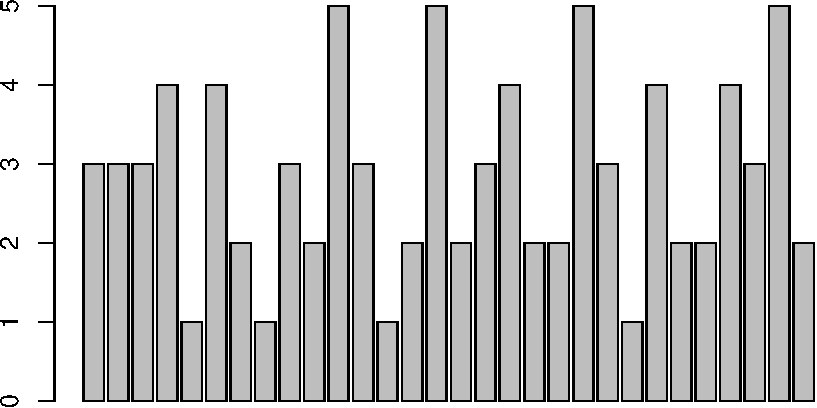
\includegraphics{01-intro_files/figure-latex/unnamed-chunk-1-18.pdf}

\begin{Shaded}
\begin{Highlighting}[]
\FunctionTok{table}\NormalTok{(x) }\CommentTok{\#制表}
\end{Highlighting}
\end{Shaded}

\begin{verbatim}
## x
## 1 2 3 4 5 
## 4 9 8 5 4
\end{verbatim}

\begin{Shaded}
\begin{Highlighting}[]
\FunctionTok{barplot}\NormalTok{(}\FunctionTok{table}\NormalTok{(x)) }\CommentTok{\#正确的图}
\end{Highlighting}
\end{Shaded}

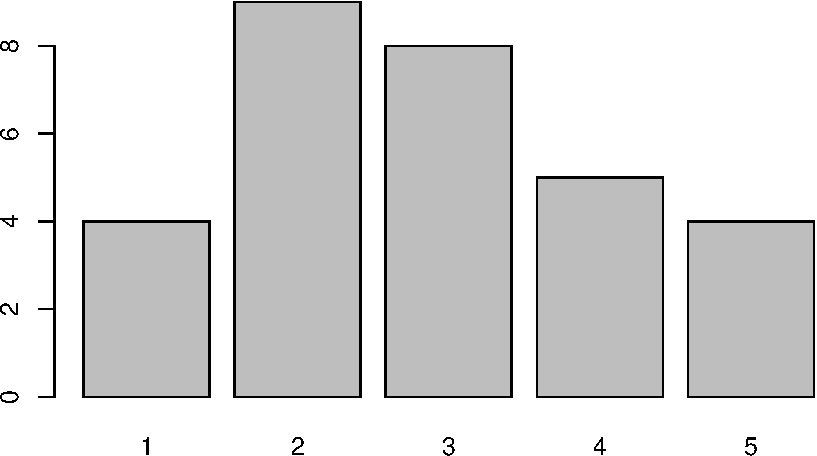
\includegraphics{01-intro_files/figure-latex/unnamed-chunk-1-19.pdf}

\begin{Shaded}
\begin{Highlighting}[]
\FunctionTok{barplot}\NormalTok{(}\FunctionTok{table}\NormalTok{(x)}\SpecialCharTok{/}\FunctionTok{length}\NormalTok{(x)) }\CommentTok{\#比例图(和上图形状一样)}
\end{Highlighting}
\end{Shaded}

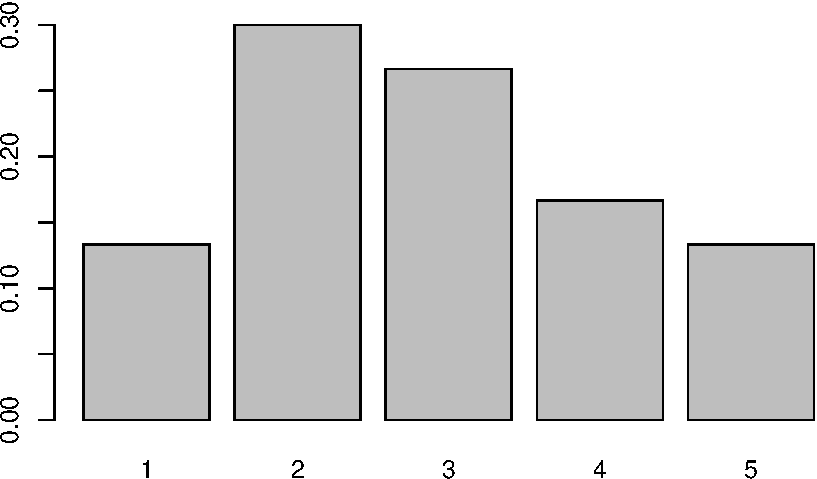
\includegraphics{01-intro_files/figure-latex/unnamed-chunk-1-20.pdf}

\begin{Shaded}
\begin{Highlighting}[]
\FunctionTok{table}\NormalTok{(x)}\SpecialCharTok{/}\FunctionTok{length}\NormalTok{(x)}
\end{Highlighting}
\end{Shaded}

\begin{verbatim}
## x
##         1         2         3         4         5 
## 0.1333333 0.3000000 0.2666667 0.1666667 0.1333333
\end{verbatim}

\begin{Shaded}
\begin{Highlighting}[]
\CommentTok{\#形成表格}
\FunctionTok{library}\NormalTok{(MASS)}\CommentTok{\#载入程序包MASS}
\NormalTok{quine }\CommentTok{\#MASS所带数据}
\end{Highlighting}
\end{Shaded}

\begin{verbatim}
##     Eth Sex Age Lrn Days
## 1     A   M  F0  SL    2
## 2     A   M  F0  SL   11
## 3     A   M  F0  SL   14
## 4     A   M  F0  AL    5
## 5     A   M  F0  AL    5
## 6     A   M  F0  AL   13
## 7     A   M  F0  AL   20
## 8     A   M  F0  AL   22
## 9     A   M  F1  SL    6
## 10    A   M  F1  SL    6
## 11    A   M  F1  SL   15
## 12    A   M  F1  AL    7
## 13    A   M  F1  AL   14
## 14    A   M  F2  SL    6
## 15    A   M  F2  SL   32
## 16    A   M  F2  SL   53
## 17    A   M  F2  SL   57
## 18    A   M  F2  AL   14
## 19    A   M  F2  AL   16
## 20    A   M  F2  AL   16
## 21    A   M  F2  AL   17
## 22    A   M  F2  AL   40
## 23    A   M  F2  AL   43
## 24    A   M  F2  AL   46
## 25    A   M  F3  AL    8
## 26    A   M  F3  AL   23
## 27    A   M  F3  AL   23
## 28    A   M  F3  AL   28
## 29    A   M  F3  AL   34
## 30    A   M  F3  AL   36
## 31    A   M  F3  AL   38
## 32    A   F  F0  SL    3
## 33    A   F  F0  AL    5
## 34    A   F  F0  AL   11
## 35    A   F  F0  AL   24
## 36    A   F  F0  AL   45
## 37    A   F  F1  SL    5
## 38    A   F  F1  SL    6
## 39    A   F  F1  SL    6
## 40    A   F  F1  SL    9
## 41    A   F  F1  SL   13
## 42    A   F  F1  SL   23
## 43    A   F  F1  SL   25
## 44    A   F  F1  SL   32
## 45    A   F  F1  SL   53
## 46    A   F  F1  SL   54
## 47    A   F  F1  AL    5
## 48    A   F  F1  AL    5
## 49    A   F  F1  AL   11
## 50    A   F  F1  AL   17
## 51    A   F  F1  AL   19
## 52    A   F  F2  SL    8
## 53    A   F  F2  SL   13
## 54    A   F  F2  SL   14
## 55    A   F  F2  SL   20
## 56    A   F  F2  SL   47
## 57    A   F  F2  SL   48
## 58    A   F  F2  SL   60
## 59    A   F  F2  SL   81
## 60    A   F  F2  AL    2
## 61    A   F  F3  AL    0
## 62    A   F  F3  AL    2
## 63    A   F  F3  AL    3
## 64    A   F  F3  AL    5
## 65    A   F  F3  AL   10
## 66    A   F  F3  AL   14
## 67    A   F  F3  AL   21
## 68    A   F  F3  AL   36
## 69    A   F  F3  AL   40
## 70    N   M  F0  SL    6
## 71    N   M  F0  SL   17
## 72    N   M  F0  SL   67
## 73    N   M  F0  AL    0
## 74    N   M  F0  AL    0
## 75    N   M  F0  AL    2
## 76    N   M  F0  AL    7
## 77    N   M  F0  AL   11
## 78    N   M  F0  AL   12
## 79    N   M  F1  SL    0
## 80    N   M  F1  SL    0
## 81    N   M  F1  SL    5
## 82    N   M  F1  SL    5
## 83    N   M  F1  SL    5
## 84    N   M  F1  SL   11
## 85    N   M  F1  SL   17
## 86    N   M  F1  AL    3
## 87    N   M  F1  AL    4
## 88    N   M  F2  SL   22
## 89    N   M  F2  SL   30
## 90    N   M  F2  SL   36
## 91    N   M  F2  AL    8
## 92    N   M  F2  AL    0
## 93    N   M  F2  AL    1
## 94    N   M  F2  AL    5
## 95    N   M  F2  AL    7
## 96    N   M  F2  AL   16
## 97    N   M  F2  AL   27
## 98    N   M  F3  AL    0
## 99    N   M  F3  AL   30
## 100   N   M  F3  AL   10
## 101   N   M  F3  AL   14
## 102   N   M  F3  AL   27
## 103   N   M  F3  AL   41
## 104   N   M  F3  AL   69
## 105   N   F  F0  SL   25
## 106   N   F  F0  AL   10
## 107   N   F  F0  AL   11
## 108   N   F  F0  AL   20
## 109   N   F  F0  AL   33
## 110   N   F  F1  SL    5
## 111   N   F  F1  SL    7
## 112   N   F  F1  SL    0
## 113   N   F  F1  SL    1
## 114   N   F  F1  SL    5
## 115   N   F  F1  SL    5
## 116   N   F  F1  SL    5
## 117   N   F  F1  SL    5
## 118   N   F  F1  SL    7
## 119   N   F  F1  SL   11
## 120   N   F  F1  SL   15
## 121   N   F  F1  AL    5
## 122   N   F  F1  AL   14
## 123   N   F  F1  AL    6
## 124   N   F  F1  AL    6
## 125   N   F  F1  AL    7
## 126   N   F  F1  AL   28
## 127   N   F  F2  SL    0
## 128   N   F  F2  SL    5
## 129   N   F  F2  SL   14
## 130   N   F  F2  SL    2
## 131   N   F  F2  SL    2
## 132   N   F  F2  SL    3
## 133   N   F  F2  SL    8
## 134   N   F  F2  SL   10
## 135   N   F  F2  SL   12
## 136   N   F  F2  AL    1
## 137   N   F  F3  AL    1
## 138   N   F  F3  AL    9
## 139   N   F  F3  AL   22
## 140   N   F  F3  AL    3
## 141   N   F  F3  AL    3
## 142   N   F  F3  AL    5
## 143   N   F  F3  AL   15
## 144   N   F  F3  AL   18
## 145   N   F  F3  AL   22
## 146   N   F  F3  AL   37
\end{verbatim}

\begin{Shaded}
\begin{Highlighting}[]
\FunctionTok{attach}\NormalTok{(quine)}\CommentTok{\#把数据变量的名字放入内存}
\CommentTok{\#下面语句产生从该数据得到的各种表格}
\FunctionTok{table}\NormalTok{(Age)}
\end{Highlighting}
\end{Shaded}

\begin{verbatim}
## Age
## F0 F1 F2 F3 
## 27 46 40 33
\end{verbatim}

\begin{Shaded}
\begin{Highlighting}[]
\FunctionTok{table}\NormalTok{(Sex, Age); tab}\OtherTok{=}\FunctionTok{xtabs}\NormalTok{(}\SpecialCharTok{\textasciitilde{}}\NormalTok{ Sex }\SpecialCharTok{+}\NormalTok{ Age, quine); }\FunctionTok{unclass}\NormalTok{(tab)}
\end{Highlighting}
\end{Shaded}

\begin{verbatim}
##    Age
## Sex F0 F1 F2 F3
##   F 10 32 19 19
##   M 17 14 21 14
\end{verbatim}

\begin{verbatim}
##    Age
## Sex F0 F1 F2 F3
##   F 10 32 19 19
##   M 17 14 21 14
## attr(,"call")
## xtabs(formula = ~Sex + Age, data = quine)
\end{verbatim}

\begin{Shaded}
\begin{Highlighting}[]
\FunctionTok{tapply}\NormalTok{(Days, Age, mean)}
\end{Highlighting}
\end{Shaded}

\begin{verbatim}
##       F0       F1       F2       F3 
## 14.85185 11.15217 21.05000 19.60606
\end{verbatim}

\begin{Shaded}
\begin{Highlighting}[]
\FunctionTok{tapply}\NormalTok{(Days, }\FunctionTok{list}\NormalTok{(Sex, Age), mean)}
\end{Highlighting}
\end{Shaded}

\begin{verbatim}
##         F0       F1       F2       F3
## F 18.70000 12.96875 18.42105 14.00000
## M 12.58824  7.00000 23.42857 27.21429
\end{verbatim}

\begin{Shaded}
\begin{Highlighting}[]
\CommentTok{\#编写简单的函数}
\CommentTok{\#下面这个函数是按照定义(编程简单, 但效率不高)求n以内的素数}
\NormalTok{ss}\OtherTok{=}\ControlFlowTok{function}\NormalTok{(}\AttributeTok{n=}\DecValTok{100}\NormalTok{)\{}
\NormalTok{  z}\OtherTok{=}\DecValTok{2}
  \ControlFlowTok{for}\NormalTok{ (i }\ControlFlowTok{in} \DecValTok{2}\SpecialCharTok{:}\NormalTok{n)}
    \ControlFlowTok{if}\NormalTok{(}\FunctionTok{any}\NormalTok{(i}\SpecialCharTok{\%\%}\DecValTok{2}\SpecialCharTok{:}\NormalTok{(i}\DecValTok{{-}1}\NormalTok{)}\SpecialCharTok{==}\DecValTok{0}\NormalTok{)}\SpecialCharTok{==}\NormalTok{F)z}\OtherTok{=}\FunctionTok{c}\NormalTok{(z,i)}
  \FunctionTok{return}\NormalTok{(z) }
\NormalTok{\}}
\CommentTok{\#fix(ss) \#用来修改任何函数或编写一个新函数}
\FunctionTok{ss}\NormalTok{() }\CommentTok{\#计算100以内的素数}
\end{Highlighting}
\end{Shaded}

\begin{verbatim}
##  [1]  2  3  5  7 11 13 17 19 23 29 31 37 41 43 47 53 59 61 67 71 73 79 83 89 97
\end{verbatim}

\begin{Shaded}
\begin{Highlighting}[]
\CommentTok{\#t1=Sys.time() \#记录时间点}
\CommentTok{\#ss(10000) \#计算10000以内的素数}
\CommentTok{\#Sys.time(){-}t1 \#计算费了多少时间}
\CommentTok{\#system.time(ss(10000))\#计算执行ss(10000)所用时间}
\CommentTok{\#函数可以不写return,这时最后一个值为return的值}
\CommentTok{\#为了输出多个值最好使用list输出}
\FunctionTok{detach}\NormalTok{(quine) }\CommentTok{\#attach的逆运行}

\CommentTok{\#画图}

\NormalTok{x}\OtherTok{=}\FunctionTok{seq}\NormalTok{(}\SpecialCharTok{{-}}\DecValTok{3}\NormalTok{,}\DecValTok{3}\NormalTok{,}\AttributeTok{len=}\DecValTok{20}\NormalTok{);y}\OtherTok{=}\FunctionTok{dnorm}\NormalTok{(x)}\CommentTok{\#产生数据}
\NormalTok{w}\OtherTok{=} \FunctionTok{data.frame}\NormalTok{(x,y)}\CommentTok{\#合并x,成为数据w}
\FunctionTok{par}\NormalTok{(}\AttributeTok{mfcol=}\FunctionTok{c}\NormalTok{(}\DecValTok{2}\NormalTok{,}\DecValTok{2}\NormalTok{))}\CommentTok{\#准备画四个图的地方}
\FunctionTok{plot}\NormalTok{(y }\SpecialCharTok{\textasciitilde{}}\NormalTok{ x, w,}\AttributeTok{main=}\StringTok{"正态密度函数"}\NormalTok{)}
\end{Highlighting}
\end{Shaded}

\begin{verbatim}
## Warning in title(...): conversion failure on '正态密度函数' in 'mbcsToSbcs': dot
## substituted for <e6>
\end{verbatim}

\begin{verbatim}
## Warning in title(...): conversion failure on '正态密度函数' in 'mbcsToSbcs': dot
## substituted for <ad>
\end{verbatim}

\begin{verbatim}
## Warning in title(...): conversion failure on '正态密度函数' in 'mbcsToSbcs': dot
## substituted for <a3>
\end{verbatim}

\begin{verbatim}
## Warning in title(...): conversion failure on '正态密度函数' in 'mbcsToSbcs': dot
## substituted for <e6>
\end{verbatim}

\begin{verbatim}
## Warning in title(...): conversion failure on '正态密度函数' in 'mbcsToSbcs': dot
## substituted for <80>
\end{verbatim}

\begin{verbatim}
## Warning in title(...): conversion failure on '正态密度函数' in 'mbcsToSbcs': dot
## substituted for <81>
\end{verbatim}

\begin{verbatim}
## Warning in title(...): conversion failure on '正态密度函数' in 'mbcsToSbcs': dot
## substituted for <e5>
\end{verbatim}

\begin{verbatim}
## Warning in title(...): conversion failure on '正态密度函数' in 'mbcsToSbcs': dot
## substituted for <af>
\end{verbatim}

\begin{verbatim}
## Warning in title(...): conversion failure on '正态密度函数' in 'mbcsToSbcs': dot
## substituted for <86>
\end{verbatim}

\begin{verbatim}
## Warning in title(...): conversion failure on '正态密度函数' in 'mbcsToSbcs': dot
## substituted for <e5>
\end{verbatim}

\begin{verbatim}
## Warning in title(...): conversion failure on '正态密度函数' in 'mbcsToSbcs': dot
## substituted for <ba>
\end{verbatim}

\begin{verbatim}
## Warning in title(...): conversion failure on '正态密度函数' in 'mbcsToSbcs': dot
## substituted for <a6>
\end{verbatim}

\begin{verbatim}
## Warning in title(...): conversion failure on '正态密度函数' in 'mbcsToSbcs': dot
## substituted for <e5>
\end{verbatim}

\begin{verbatim}
## Warning in title(...): conversion failure on '正态密度函数' in 'mbcsToSbcs': dot
## substituted for <87>
\end{verbatim}

\begin{verbatim}
## Warning in title(...): conversion failure on '正态密度函数' in 'mbcsToSbcs': dot
## substituted for <bd>
\end{verbatim}

\begin{verbatim}
## Warning in title(...): conversion failure on '正态密度函数' in 'mbcsToSbcs': dot
## substituted for <e6>
\end{verbatim}

\begin{verbatim}
## Warning in title(...): conversion failure on '正态密度函数' in 'mbcsToSbcs': dot
## substituted for <95>
\end{verbatim}

\begin{verbatim}
## Warning in title(...): conversion failure on '正态密度函数' in 'mbcsToSbcs': dot
## substituted for <b0>
\end{verbatim}

\begin{Shaded}
\begin{Highlighting}[]
\FunctionTok{plot}\NormalTok{(y }\SpecialCharTok{\textasciitilde{}}\NormalTok{ x,w,}\AttributeTok{type=}\StringTok{"l"}\NormalTok{, }\AttributeTok{main=}\StringTok{"正态密度函数"}\NormalTok{)}
\end{Highlighting}
\end{Shaded}

\begin{verbatim}
## Warning in title(...): conversion failure on '正态密度函数' in 'mbcsToSbcs': dot
## substituted for <e6>
\end{verbatim}

\begin{verbatim}
## Warning in title(...): conversion failure on '正态密度函数' in 'mbcsToSbcs': dot
## substituted for <ad>
\end{verbatim}

\begin{verbatim}
## Warning in title(...): conversion failure on '正态密度函数' in 'mbcsToSbcs': dot
## substituted for <a3>
\end{verbatim}

\begin{verbatim}
## Warning in title(...): conversion failure on '正态密度函数' in 'mbcsToSbcs': dot
## substituted for <e6>
\end{verbatim}

\begin{verbatim}
## Warning in title(...): conversion failure on '正态密度函数' in 'mbcsToSbcs': dot
## substituted for <80>
\end{verbatim}

\begin{verbatim}
## Warning in title(...): conversion failure on '正态密度函数' in 'mbcsToSbcs': dot
## substituted for <81>
\end{verbatim}

\begin{verbatim}
## Warning in title(...): conversion failure on '正态密度函数' in 'mbcsToSbcs': dot
## substituted for <e5>
\end{verbatim}

\begin{verbatim}
## Warning in title(...): conversion failure on '正态密度函数' in 'mbcsToSbcs': dot
## substituted for <af>
\end{verbatim}

\begin{verbatim}
## Warning in title(...): conversion failure on '正态密度函数' in 'mbcsToSbcs': dot
## substituted for <86>
\end{verbatim}

\begin{verbatim}
## Warning in title(...): conversion failure on '正态密度函数' in 'mbcsToSbcs': dot
## substituted for <e5>
\end{verbatim}

\begin{verbatim}
## Warning in title(...): conversion failure on '正态密度函数' in 'mbcsToSbcs': dot
## substituted for <ba>
\end{verbatim}

\begin{verbatim}
## Warning in title(...): conversion failure on '正态密度函数' in 'mbcsToSbcs': dot
## substituted for <a6>
\end{verbatim}

\begin{verbatim}
## Warning in title(...): conversion failure on '正态密度函数' in 'mbcsToSbcs': dot
## substituted for <e5>
\end{verbatim}

\begin{verbatim}
## Warning in title(...): conversion failure on '正态密度函数' in 'mbcsToSbcs': dot
## substituted for <87>
\end{verbatim}

\begin{verbatim}
## Warning in title(...): conversion failure on '正态密度函数' in 'mbcsToSbcs': dot
## substituted for <bd>
\end{verbatim}

\begin{verbatim}
## Warning in title(...): conversion failure on '正态密度函数' in 'mbcsToSbcs': dot
## substituted for <e6>
\end{verbatim}

\begin{verbatim}
## Warning in title(...): conversion failure on '正态密度函数' in 'mbcsToSbcs': dot
## substituted for <95>
\end{verbatim}

\begin{verbatim}
## Warning in title(...): conversion failure on '正态密度函数' in 'mbcsToSbcs': dot
## substituted for <b0>
\end{verbatim}

\begin{Shaded}
\begin{Highlighting}[]
\FunctionTok{plot}\NormalTok{(y }\SpecialCharTok{\textasciitilde{}}\NormalTok{ x,w,}\AttributeTok{type=}\StringTok{"o"}\NormalTok{, }\AttributeTok{main=}\StringTok{"正态密度函数"}\NormalTok{)}
\end{Highlighting}
\end{Shaded}

\begin{verbatim}
## Warning in title(...): conversion failure on '正态密度函数' in 'mbcsToSbcs': dot
## substituted for <e6>
\end{verbatim}

\begin{verbatim}
## Warning in title(...): conversion failure on '正态密度函数' in 'mbcsToSbcs': dot
## substituted for <ad>
\end{verbatim}

\begin{verbatim}
## Warning in title(...): conversion failure on '正态密度函数' in 'mbcsToSbcs': dot
## substituted for <a3>
\end{verbatim}

\begin{verbatim}
## Warning in title(...): conversion failure on '正态密度函数' in 'mbcsToSbcs': dot
## substituted for <e6>
\end{verbatim}

\begin{verbatim}
## Warning in title(...): conversion failure on '正态密度函数' in 'mbcsToSbcs': dot
## substituted for <80>
\end{verbatim}

\begin{verbatim}
## Warning in title(...): conversion failure on '正态密度函数' in 'mbcsToSbcs': dot
## substituted for <81>
\end{verbatim}

\begin{verbatim}
## Warning in title(...): conversion failure on '正态密度函数' in 'mbcsToSbcs': dot
## substituted for <e5>
\end{verbatim}

\begin{verbatim}
## Warning in title(...): conversion failure on '正态密度函数' in 'mbcsToSbcs': dot
## substituted for <af>
\end{verbatim}

\begin{verbatim}
## Warning in title(...): conversion failure on '正态密度函数' in 'mbcsToSbcs': dot
## substituted for <86>
\end{verbatim}

\begin{verbatim}
## Warning in title(...): conversion failure on '正态密度函数' in 'mbcsToSbcs': dot
## substituted for <e5>
\end{verbatim}

\begin{verbatim}
## Warning in title(...): conversion failure on '正态密度函数' in 'mbcsToSbcs': dot
## substituted for <ba>
\end{verbatim}

\begin{verbatim}
## Warning in title(...): conversion failure on '正态密度函数' in 'mbcsToSbcs': dot
## substituted for <a6>
\end{verbatim}

\begin{verbatim}
## Warning in title(...): conversion failure on '正态密度函数' in 'mbcsToSbcs': dot
## substituted for <e5>
\end{verbatim}

\begin{verbatim}
## Warning in title(...): conversion failure on '正态密度函数' in 'mbcsToSbcs': dot
## substituted for <87>
\end{verbatim}

\begin{verbatim}
## Warning in title(...): conversion failure on '正态密度函数' in 'mbcsToSbcs': dot
## substituted for <bd>
\end{verbatim}

\begin{verbatim}
## Warning in title(...): conversion failure on '正态密度函数' in 'mbcsToSbcs': dot
## substituted for <e6>
\end{verbatim}

\begin{verbatim}
## Warning in title(...): conversion failure on '正态密度函数' in 'mbcsToSbcs': dot
## substituted for <95>
\end{verbatim}

\begin{verbatim}
## Warning in title(...): conversion failure on '正态密度函数' in 'mbcsToSbcs': dot
## substituted for <b0>
\end{verbatim}

\begin{Shaded}
\begin{Highlighting}[]
\FunctionTok{plot}\NormalTok{(y }\SpecialCharTok{\textasciitilde{}}\NormalTok{ x,w,}\AttributeTok{type=}\StringTok{"b"}\NormalTok{,}\AttributeTok{main=}\StringTok{"正态密度函数"}\NormalTok{)}
\end{Highlighting}
\end{Shaded}

\begin{verbatim}
## Warning in title(...): conversion failure on '正态密度函数' in 'mbcsToSbcs': dot
## substituted for <e6>
\end{verbatim}

\begin{verbatim}
## Warning in title(...): conversion failure on '正态密度函数' in 'mbcsToSbcs': dot
## substituted for <ad>
\end{verbatim}

\begin{verbatim}
## Warning in title(...): conversion failure on '正态密度函数' in 'mbcsToSbcs': dot
## substituted for <a3>
\end{verbatim}

\begin{verbatim}
## Warning in title(...): conversion failure on '正态密度函数' in 'mbcsToSbcs': dot
## substituted for <e6>
\end{verbatim}

\begin{verbatim}
## Warning in title(...): conversion failure on '正态密度函数' in 'mbcsToSbcs': dot
## substituted for <80>
\end{verbatim}

\begin{verbatim}
## Warning in title(...): conversion failure on '正态密度函数' in 'mbcsToSbcs': dot
## substituted for <81>
\end{verbatim}

\begin{verbatim}
## Warning in title(...): conversion failure on '正态密度函数' in 'mbcsToSbcs': dot
## substituted for <e5>
\end{verbatim}

\begin{verbatim}
## Warning in title(...): conversion failure on '正态密度函数' in 'mbcsToSbcs': dot
## substituted for <af>
\end{verbatim}

\begin{verbatim}
## Warning in title(...): conversion failure on '正态密度函数' in 'mbcsToSbcs': dot
## substituted for <86>
\end{verbatim}

\begin{verbatim}
## Warning in title(...): conversion failure on '正态密度函数' in 'mbcsToSbcs': dot
## substituted for <e5>
\end{verbatim}

\begin{verbatim}
## Warning in title(...): conversion failure on '正态密度函数' in 'mbcsToSbcs': dot
## substituted for <ba>
\end{verbatim}

\begin{verbatim}
## Warning in title(...): conversion failure on '正态密度函数' in 'mbcsToSbcs': dot
## substituted for <a6>
\end{verbatim}

\begin{verbatim}
## Warning in title(...): conversion failure on '正态密度函数' in 'mbcsToSbcs': dot
## substituted for <e5>
\end{verbatim}

\begin{verbatim}
## Warning in title(...): conversion failure on '正态密度函数' in 'mbcsToSbcs': dot
## substituted for <87>
\end{verbatim}

\begin{verbatim}
## Warning in title(...): conversion failure on '正态密度函数' in 'mbcsToSbcs': dot
## substituted for <bd>
\end{verbatim}

\begin{verbatim}
## Warning in title(...): conversion failure on '正态密度函数' in 'mbcsToSbcs': dot
## substituted for <e6>
\end{verbatim}

\begin{verbatim}
## Warning in title(...): conversion failure on '正态密度函数' in 'mbcsToSbcs': dot
## substituted for <95>
\end{verbatim}

\begin{verbatim}
## Warning in title(...): conversion failure on '正态密度函数' in 'mbcsToSbcs': dot
## substituted for <b0>
\end{verbatim}

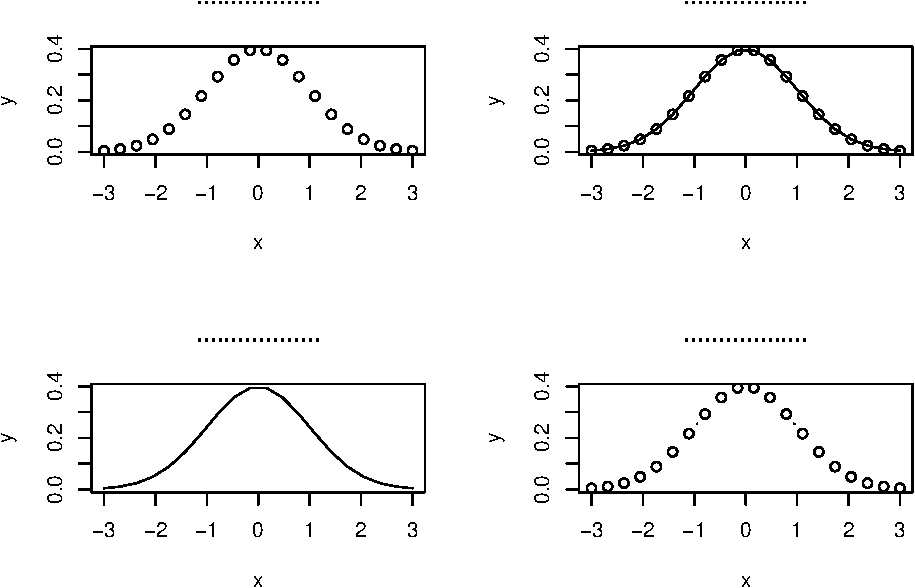
\includegraphics{01-intro_files/figure-latex/unnamed-chunk-1-21.pdf}

\begin{Shaded}
\begin{Highlighting}[]
\FunctionTok{par}\NormalTok{(}\AttributeTok{mfcol=}\FunctionTok{c}\NormalTok{(}\DecValTok{1}\NormalTok{,}\DecValTok{1}\NormalTok{))}\CommentTok{\#取消par(mfcol=c(2,2))}

\CommentTok{\#色彩和符号等的调整}
\FunctionTok{plot}\NormalTok{(}\DecValTok{1}\NormalTok{,}\DecValTok{1}\NormalTok{,}\AttributeTok{xlim=}\FunctionTok{c}\NormalTok{(}\DecValTok{1}\NormalTok{,}\FloatTok{7.5}\NormalTok{),}\AttributeTok{ylim=}\FunctionTok{c}\NormalTok{(}\DecValTok{0}\NormalTok{,}\DecValTok{5}\NormalTok{),}\AttributeTok{type=}\StringTok{"n"}\NormalTok{) }\CommentTok{\#画出框架}
\CommentTok{\#在plot命令后面追加点(如要追加线可用lines函数):}
\FunctionTok{points}\NormalTok{(}\DecValTok{1}\SpecialCharTok{:}\DecValTok{7}\NormalTok{,}\FunctionTok{rep}\NormalTok{(}\FloatTok{4.5}\NormalTok{,}\DecValTok{7}\NormalTok{),}\AttributeTok{cex=}\FunctionTok{seq}\NormalTok{(}\DecValTok{1}\NormalTok{,}\DecValTok{4}\NormalTok{,}\AttributeTok{l=}\DecValTok{7}\NormalTok{),}\AttributeTok{col=}\DecValTok{1}\SpecialCharTok{:}\DecValTok{7}\NormalTok{, }\AttributeTok{pch=}\DecValTok{0}\SpecialCharTok{:}\DecValTok{6}\NormalTok{)}
\FunctionTok{text}\NormalTok{(}\DecValTok{1}\SpecialCharTok{:}\DecValTok{7}\NormalTok{,}\FunctionTok{rep}\NormalTok{(}\FloatTok{3.5}\NormalTok{,}\DecValTok{7}\NormalTok{),}\AttributeTok{labels=}\FunctionTok{paste}\NormalTok{(}\DecValTok{0}\SpecialCharTok{:}\DecValTok{6}\NormalTok{,letters[}\DecValTok{1}\SpecialCharTok{:}\DecValTok{7}\NormalTok{]),}
\AttributeTok{cex=}\FunctionTok{seq}\NormalTok{(}\DecValTok{1}\NormalTok{,}\DecValTok{4}\NormalTok{,}\AttributeTok{l=}\DecValTok{7}\NormalTok{),}\AttributeTok{col=}\DecValTok{1}\SpecialCharTok{:}\DecValTok{7}\NormalTok{)}\CommentTok{\#在指定位置加文字}
\FunctionTok{points}\NormalTok{(}\DecValTok{1}\SpecialCharTok{:}\DecValTok{7}\NormalTok{,}\FunctionTok{rep}\NormalTok{(}\DecValTok{2}\NormalTok{,}\DecValTok{7}\NormalTok{), }\AttributeTok{pch=}\NormalTok{(}\DecValTok{0}\SpecialCharTok{:}\DecValTok{6}\NormalTok{)}\SpecialCharTok{+}\DecValTok{7}\NormalTok{)}\CommentTok{\#点出符号7到13}
\FunctionTok{text}\NormalTok{((}\DecValTok{1}\SpecialCharTok{:}\DecValTok{7}\NormalTok{)}\SpecialCharTok{+}\FloatTok{0.25}\NormalTok{, }\FunctionTok{rep}\NormalTok{(}\DecValTok{2}\NormalTok{,}\DecValTok{7}\NormalTok{), }\FunctionTok{paste}\NormalTok{((}\DecValTok{0}\SpecialCharTok{:}\DecValTok{6}\NormalTok{)}\SpecialCharTok{+}\DecValTok{7}\NormalTok{))}\CommentTok{\#加符号号码}
\FunctionTok{points}\NormalTok{(}\DecValTok{1}\SpecialCharTok{:}\DecValTok{7}\NormalTok{,}\FunctionTok{rep}\NormalTok{(}\DecValTok{1}\NormalTok{,}\DecValTok{7}\NormalTok{), }\AttributeTok{pch=}\NormalTok{(}\DecValTok{0}\SpecialCharTok{:}\DecValTok{6}\NormalTok{)}\SpecialCharTok{+}\DecValTok{14}\NormalTok{) }\CommentTok{\#点出符号14到20}
\FunctionTok{text}\NormalTok{((}\DecValTok{1}\SpecialCharTok{:}\DecValTok{7}\NormalTok{)}\SpecialCharTok{+}\FloatTok{0.25}\NormalTok{, }\FunctionTok{rep}\NormalTok{(}\DecValTok{1}\NormalTok{,}\DecValTok{7}\NormalTok{), }\FunctionTok{paste}\NormalTok{((}\DecValTok{0}\SpecialCharTok{:}\DecValTok{6}\NormalTok{)}\SpecialCharTok{+}\DecValTok{14}\NormalTok{)) }\CommentTok{\#加符号号码}
\end{Highlighting}
\end{Shaded}

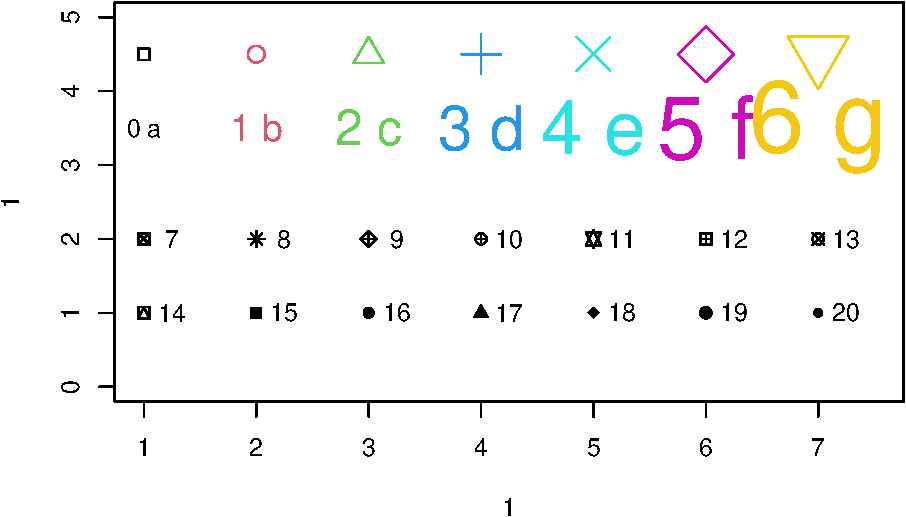
\includegraphics{01-intro_files/figure-latex/unnamed-chunk-1-22.pdf}

\begin{Shaded}
\begin{Highlighting}[]
\CommentTok{\#关于符号形状、大小、颜色以及其他画图选项的说明可用"?par"来查看}
\end{Highlighting}
\end{Shaded}

\hypertarget{pythonux8bedux8a00ux5b89ux88c5ux53caux73afux5883ux914dux7f6e}{%
\subsection{python语言安装及环境配置}\label{pythonux8bedux8a00ux5b89ux88c5ux53caux73afux5883ux914dux7f6e}}

\begin{itemize}
\tightlist
\item
  直接安装Anaconda编辑环境;
\item
  python基础;
\end{itemize}

\begin{Shaded}
\begin{Highlighting}[]
\NormalTok{x }\OperatorTok{=}\NormalTok{ [}\DecValTok{1}\NormalTok{,}\DecValTok{2}\NormalTok{,}\DecValTok{3}\NormalTok{,}\DecValTok{4}\NormalTok{]}
\BuiltInTok{print}\NormalTok{(x[}\DecValTok{2}\NormalTok{])}
\end{Highlighting}
\end{Shaded}

\begin{verbatim}
## 3
\end{verbatim}

\hypertarget{ux6570ux636eux63cfux8ff0}{%
\chapter{数据描述}\label{ux6570ux636eux63cfux8ff0}}

\hypertarget{ux6570ux636eux7684ux610fux4e49ux53caux83b7ux53d6}{%
\subsection{数据的意义及获取}\label{ux6570ux636eux7684ux610fux4e49ux53caux83b7ux53d6}}

\begin{enumerate}
\def\labelenumi{\arabic{enumi}.}
\tightlist
\item
  数据的类型:使用不同的标准,可将数据分成不同的类型,如数量型和质量型;

  \begin{itemize}
  \tightlist
  \item
    质量型(Categorical):定类变量(Nominal)、定序变量(Ordinal);
  \item
    数量型(Numerical):定距数据(interval data)、等比变量(ratio);
  \end{itemize}
\item
  数据的获取:实验数据、观察数据、网络抓取及公用数据库(UCI,kaggle)等;

  \begin{itemize}
  \tightlist
  \item
    datalist(\href{https://www.datasetlist.com/}{datalist})汇集了多 个网站上的数据集;
  \item
    UCI数据库(\href{http://archive.ics.uci.edu/ml/datasets.php}{uci dataset}):创建于1987年,是一个比较有历史的数据集数据库,是一个含有数据库、领域知识及数据产生器的网站;
  \item
    Fastai(\href{https://course.fast.ai/datasets}{Fastai}):进行图像分类、NLP及图像定位(image localization)的数据集;
  \item
    Kaggle(\href{https://www.kaggle.com/datasets}{kaggle}):数据科学竞赛的主要网站;
  \item
    Sklearn(\href{https://scikit-learn.org/stable/}{Skearn}):数据科学非常重要的包;
  \end{itemize}
\item
  数据的产生过程:总体(有限、无限,未知)和样本(总体的子集,随机性,已知);
  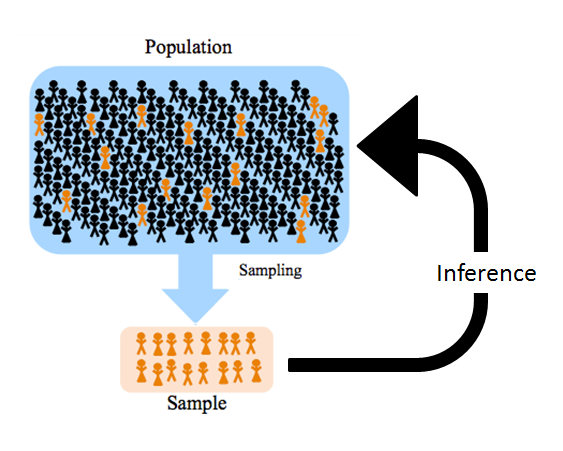
\includegraphics{pics/population-sample.png}
\item
  表格型数据(结构化数据):行(样本数量,rows), 列(变量名,columns)
\end{enumerate}

\begin{Shaded}
\begin{Highlighting}[]
\FunctionTok{library}\NormalTok{(ISLR)}
\CommentTok{\#View(Auto)}
\FunctionTok{head}\NormalTok{(Auto) }\CommentTok{\# 查看数据的前5行}
\end{Highlighting}
\end{Shaded}

\begin{verbatim}
##   mpg cylinders displacement horsepower weight acceleration year origin
## 1  18         8          307        130   3504         12.0   70      1
## 2  15         8          350        165   3693         11.5   70      1
## 3  18         8          318        150   3436         11.0   70      1
## 4  16         8          304        150   3433         12.0   70      1
## 5  17         8          302        140   3449         10.5   70      1
## 6  15         8          429        198   4341         10.0   70      1
##                        name
## 1 chevrolet chevelle malibu
## 2         buick skylark 320
## 3        plymouth satellite
## 4             amc rebel sst
## 5               ford torino
## 6          ford galaxie 500
\end{verbatim}

\begin{Shaded}
\begin{Highlighting}[]
\FunctionTok{names}\NormalTok{(Auto) }\CommentTok{\# 查看变量名}
\end{Highlighting}
\end{Shaded}

\begin{verbatim}
## [1] "mpg"          "cylinders"    "displacement" "horsepower"   "weight"      
## [6] "acceleration" "year"         "origin"       "name"
\end{verbatim}

\hypertarget{ux7b80ux5355ux7684ux6570ux636eux6c47ux603b}{%
\subsection{简单的数据汇总}\label{ux7b80ux5355ux7684ux6570ux636eux6c47ux603b}}

\begin{Shaded}
\begin{Highlighting}[]
\FunctionTok{library}\NormalTok{(ISLR)}
\FunctionTok{summary}\NormalTok{(Auto)}
\end{Highlighting}
\end{Shaded}

\begin{verbatim}
##       mpg          cylinders      displacement     horsepower        weight    
##  Min.   : 9.00   Min.   :3.000   Min.   : 68.0   Min.   : 46.0   Min.   :1613  
##  1st Qu.:17.00   1st Qu.:4.000   1st Qu.:105.0   1st Qu.: 75.0   1st Qu.:2225  
##  Median :22.75   Median :4.000   Median :151.0   Median : 93.5   Median :2804  
##  Mean   :23.45   Mean   :5.472   Mean   :194.4   Mean   :104.5   Mean   :2978  
##  3rd Qu.:29.00   3rd Qu.:8.000   3rd Qu.:275.8   3rd Qu.:126.0   3rd Qu.:3615  
##  Max.   :46.60   Max.   :8.000   Max.   :455.0   Max.   :230.0   Max.   :5140  
##                                                                                
##   acceleration        year           origin                      name    
##  Min.   : 8.00   Min.   :70.00   Min.   :1.000   amc matador       :  5  
##  1st Qu.:13.78   1st Qu.:73.00   1st Qu.:1.000   ford pinto        :  5  
##  Median :15.50   Median :76.00   Median :1.000   toyota corolla    :  5  
##  Mean   :15.54   Mean   :75.98   Mean   :1.577   amc gremlin       :  4  
##  3rd Qu.:17.02   3rd Qu.:79.00   3rd Qu.:2.000   amc hornet        :  4  
##  Max.   :24.80   Max.   :82.00   Max.   :3.000   chevrolet chevette:  4  
##                                                  (Other)           :365
\end{verbatim}

\begin{Shaded}
\begin{Highlighting}[]
\FunctionTok{mean}\NormalTok{(Auto}\SpecialCharTok{$}\NormalTok{mpg)}
\end{Highlighting}
\end{Shaded}

\begin{verbatim}
## [1] 23.44592
\end{verbatim}

\begin{itemize}
\item
  样本平均值的计算:\[\bar{Y}=\frac{1}{n}\sum\limits_{i=1}^ny_i\]
\item
  样本的方差:\[s^2=\frac{1}{n-1}\sum\limits_{i=1}^n(x_i-\bar{x})^2\]
\item
  线性相关系数:\[r=\frac{\sum\limits_{i=1}^n(x_i-\bar{x})(y_i-\bar{y})}{\sqrt{\sum\limits_{i=1}^n(x_i-\bar{x})^2}\sqrt{\sum\limits_{i=1}^n(y_i-\bar{y})^2}}\]
\item
  课堂练习:
  统计7位同学周未的学习时间,数据为:8,11,7,13,9,5,9,计算同学学习时间的均值,中位数、四分位数、标准差和极差(使用手算)。

  \begin{itemize}
  \tightlist
  \item
    \(\bar{x}=\frac{8+11+7+13+9+5+9}{7}=8.85\)
  \item
    \(s^2=\frac{(8-8.85)^2+\cdots+(9-8.85)^2}{7-1}=6.81\)
  \item
    \(s=\sqrt{s^2}=\sqrt{6.81}=2.6\)
  \item
    Median = 9; Mode = 9; Range = Max - min = 13-5=8
  \end{itemize}
\end{itemize}

\begin{Shaded}
\begin{Highlighting}[]
\NormalTok{d }\OtherTok{\textless{}{-}} \FunctionTok{c}\NormalTok{(}\DecValTok{8}\NormalTok{,}\DecValTok{11}\NormalTok{,}\DecValTok{7}\NormalTok{,}\DecValTok{13}\NormalTok{,}\DecValTok{9}\NormalTok{,}\DecValTok{5}\NormalTok{,}\DecValTok{9}\NormalTok{)}
\FunctionTok{mean}\NormalTok{(d)}
\end{Highlighting}
\end{Shaded}

\begin{verbatim}
## [1] 8.857143
\end{verbatim}

\begin{Shaded}
\begin{Highlighting}[]
\FunctionTok{median}\NormalTok{(d)}
\end{Highlighting}
\end{Shaded}

\begin{verbatim}
## [1] 9
\end{verbatim}

\begin{Shaded}
\begin{Highlighting}[]
\FunctionTok{mode}\NormalTok{(d)}
\end{Highlighting}
\end{Shaded}

\begin{verbatim}
## [1] "numeric"
\end{verbatim}

\begin{Shaded}
\begin{Highlighting}[]
\FunctionTok{quantile}\NormalTok{(d)}
\end{Highlighting}
\end{Shaded}

\begin{verbatim}
##   0%  25%  50%  75% 100% 
##  5.0  7.5  9.0 10.0 13.0
\end{verbatim}

\begin{Shaded}
\begin{Highlighting}[]
\FunctionTok{sd}\NormalTok{(d)}
\end{Highlighting}
\end{Shaded}

\begin{verbatim}
## [1] 2.609506
\end{verbatim}

\hypertarget{ux6570ux636eux7684ux53efux89c6ux5316}{%
\subsection{数据的可视化}\label{ux6570ux636eux7684ux53efux89c6ux5316}}

\begin{enumerate}
\def\labelenumi{\arabic{enumi}.}
\tightlist
\item
  两个变量之间的关系:散点图(scatter)
\end{enumerate}

\begin{Shaded}
\begin{Highlighting}[]
\FunctionTok{library}\NormalTok{(ISLR)}
\FunctionTok{plot}\NormalTok{(Auto}\SpecialCharTok{$}\NormalTok{mpg,Auto}\SpecialCharTok{$}\NormalTok{horsepower)}
\end{Highlighting}
\end{Shaded}

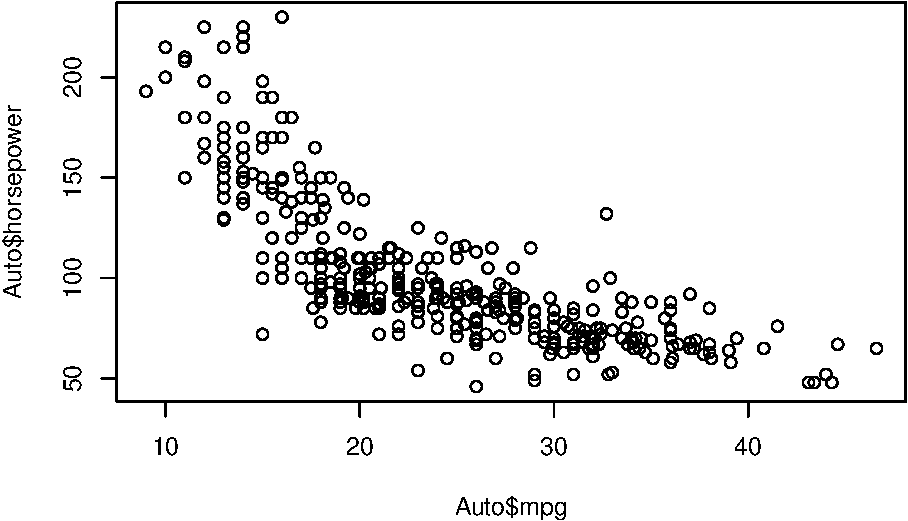
\includegraphics{02-literature_files/figure-latex/scatter-1.pdf}
2. 描述数量变量数据分布情况的图形:直方图(histogram)

\begin{Shaded}
\begin{Highlighting}[]
\FunctionTok{par}\NormalTok{(}\AttributeTok{mfrow=}\FunctionTok{c}\NormalTok{(}\DecValTok{1}\NormalTok{,}\DecValTok{2}\NormalTok{))}
\FunctionTok{hist}\NormalTok{(Auto}\SpecialCharTok{$}\NormalTok{horsepower)}
\FunctionTok{hist}\NormalTok{(Auto}\SpecialCharTok{$}\NormalTok{mpg)}
\end{Highlighting}
\end{Shaded}

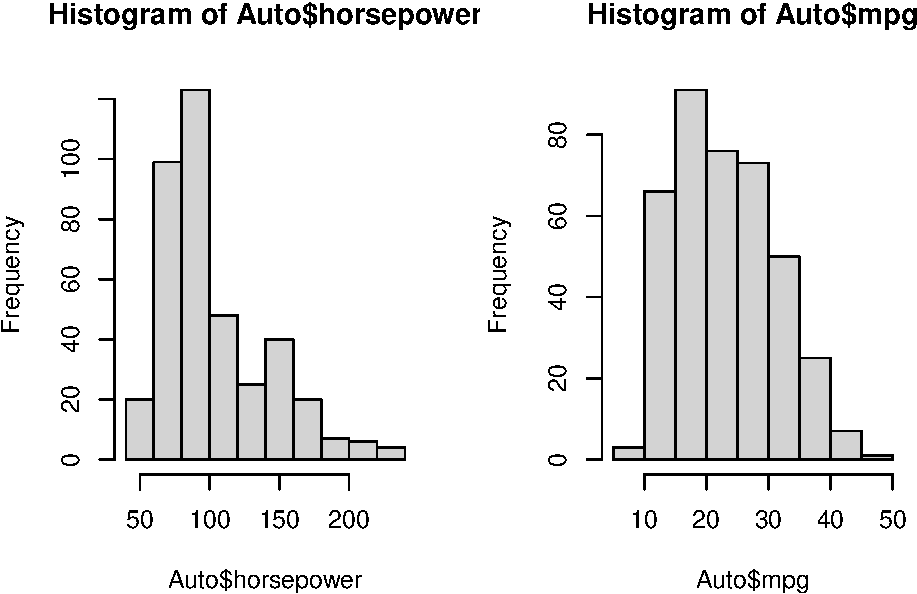
\includegraphics{02-literature_files/figure-latex/histogram-1.pdf}
3. 描述数量变量数据分布情况的图形:盒形图或箱线图(boxplot)

\begin{Shaded}
\begin{Highlighting}[]
\FunctionTok{boxplot}\NormalTok{(Auto}\SpecialCharTok{$}\NormalTok{horsepower)}
\end{Highlighting}
\end{Shaded}

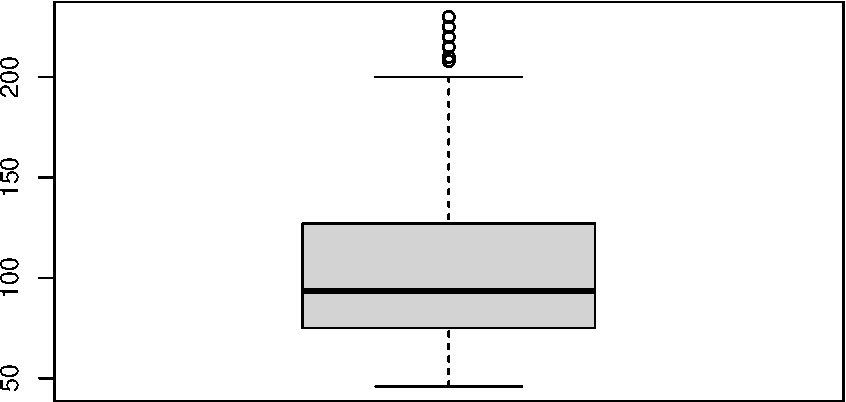
\includegraphics{02-literature_files/figure-latex/boxplot-1.pdf}
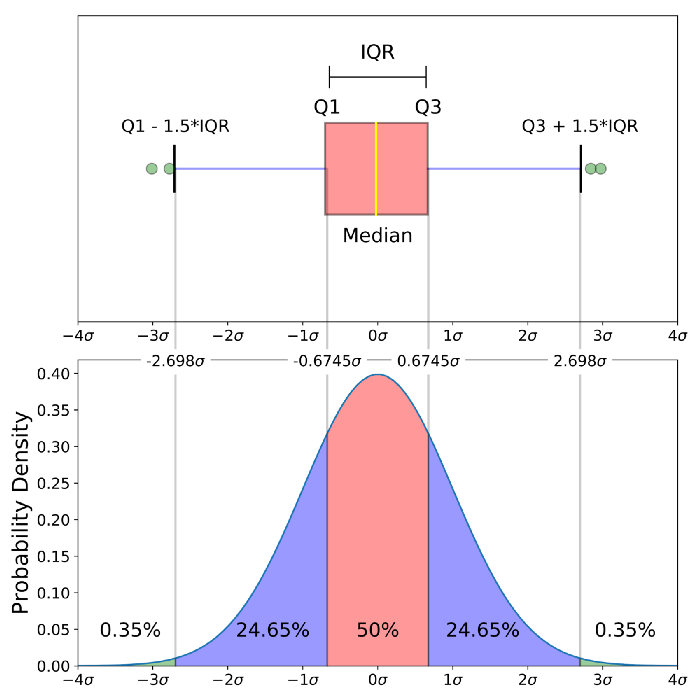
\includegraphics{pics/boxplot.png}
4. 把一些数目以矩形形式显示, 表面上类似于直方图, 但直方图是描述连续数量变量的, 而条形图描述离散变量或分类变量各个水平计数(频数):条形图(barplot)。

\begin{Shaded}
\begin{Highlighting}[]
\CommentTok{\# Simple Bar Plot}
\NormalTok{counts }\OtherTok{\textless{}{-}} \FunctionTok{table}\NormalTok{(mtcars}\SpecialCharTok{$}\NormalTok{gear)}
\FunctionTok{barplot}\NormalTok{(counts, }\AttributeTok{main=}\StringTok{"Car Distribution"}\NormalTok{,}
   \AttributeTok{xlab=}\StringTok{"Number of Gears"}\NormalTok{)}
\end{Highlighting}
\end{Shaded}

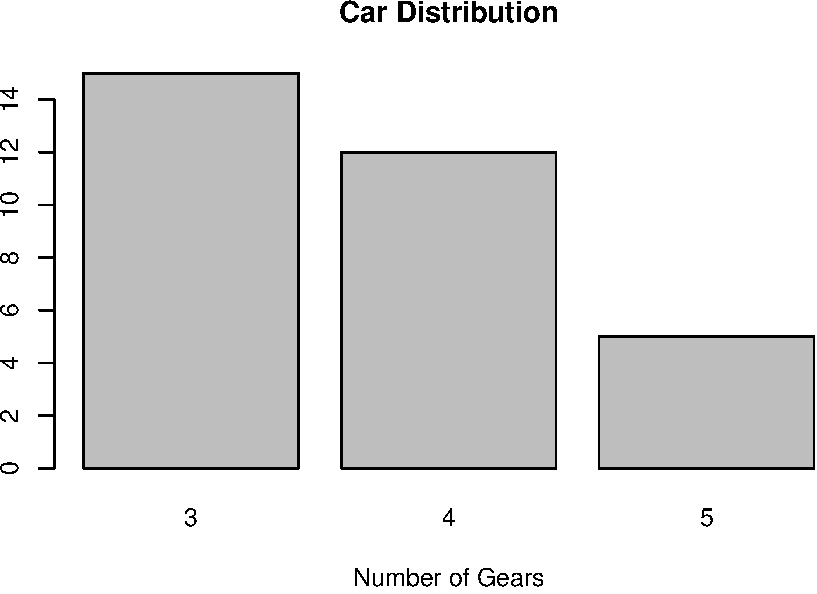
\includegraphics{02-literature_files/figure-latex/barplot-1.pdf}

\begin{enumerate}
\def\labelenumi{\arabic{enumi}.}
\setcounter{enumi}{4}
\tightlist
\item
  ggplot2(\href{https://ggplot2.tidyverse.org/index.html}{ggplot2}):ggplot2是一个用于声明性地创建图形的系统,基于图形语法。你提供数据,告诉ggplot2如何将变量映射到美学上,使用什么图形基元,它就会处理好这些细节。
\end{enumerate}

\begin{itemize}
\tightlist
\item
  一个简单的ggplot2例子
\end{itemize}

\begin{Shaded}
\begin{Highlighting}[]
\FunctionTok{library}\NormalTok{(ggplot2)}
\FunctionTok{ggplot}\NormalTok{(mpg, }\FunctionTok{aes}\NormalTok{(displ, hwy, }\AttributeTok{colour =}\NormalTok{ class)) }\SpecialCharTok{+} 
  \FunctionTok{geom\_point}\NormalTok{()}
\end{Highlighting}
\end{Shaded}

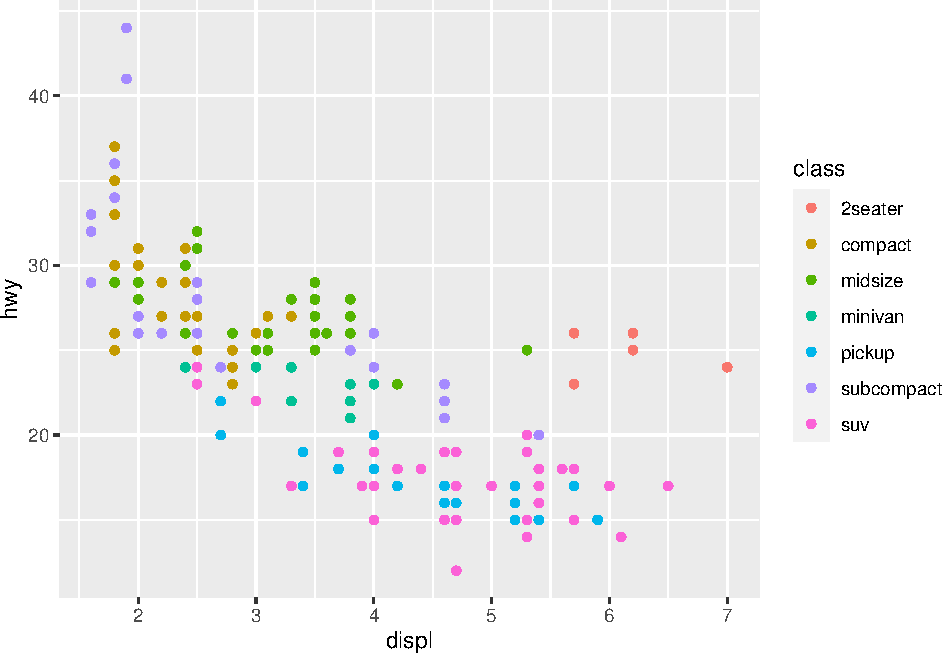
\includegraphics{02-literature_files/figure-latex/ggplot01-1.pdf}

\begin{Shaded}
\begin{Highlighting}[]
\CommentTok{\# Generate some sample data, then compute mean and standard deviation}
\CommentTok{\# in each group}
\NormalTok{df }\OtherTok{\textless{}{-}} \FunctionTok{data.frame}\NormalTok{(}
  \AttributeTok{gp =} \FunctionTok{factor}\NormalTok{(}\FunctionTok{rep}\NormalTok{(letters[}\DecValTok{1}\SpecialCharTok{:}\DecValTok{3}\NormalTok{], }\AttributeTok{each =} \DecValTok{10}\NormalTok{)),}
  \AttributeTok{y =} \FunctionTok{rnorm}\NormalTok{(}\DecValTok{30}\NormalTok{)}
\NormalTok{)}
\NormalTok{ds }\OtherTok{\textless{}{-}} \FunctionTok{do.call}\NormalTok{(rbind, }\FunctionTok{lapply}\NormalTok{(}\FunctionTok{split}\NormalTok{(df, df}\SpecialCharTok{$}\NormalTok{gp), }\ControlFlowTok{function}\NormalTok{(d) \{}
  \FunctionTok{data.frame}\NormalTok{(}\AttributeTok{mean =} \FunctionTok{mean}\NormalTok{(d}\SpecialCharTok{$}\NormalTok{y), }\AttributeTok{sd =} \FunctionTok{sd}\NormalTok{(d}\SpecialCharTok{$}\NormalTok{y), }\AttributeTok{gp =}\NormalTok{ d}\SpecialCharTok{$}\NormalTok{gp)}
\NormalTok{\}))}

\CommentTok{\# The summary data frame ds is used to plot larger red points on top}
\CommentTok{\# of the raw data. Note that we don\textquotesingle{}t need to supply \textasciigrave{}data\textasciigrave{} or \textasciigrave{}mapping\textasciigrave{}}
\CommentTok{\# in each layer because the defaults from ggplot() are used.}
\FunctionTok{ggplot}\NormalTok{(df, }\FunctionTok{aes}\NormalTok{(gp, y)) }\SpecialCharTok{+}
  \FunctionTok{geom\_point}\NormalTok{() }\SpecialCharTok{+}
  \FunctionTok{geom\_point}\NormalTok{(}\AttributeTok{data =}\NormalTok{ ds, }\FunctionTok{aes}\NormalTok{(}\AttributeTok{y =}\NormalTok{ mean), }\AttributeTok{colour =} \StringTok{\textquotesingle{}red\textquotesingle{}}\NormalTok{, }\AttributeTok{size =} \DecValTok{3}\NormalTok{)}
\end{Highlighting}
\end{Shaded}

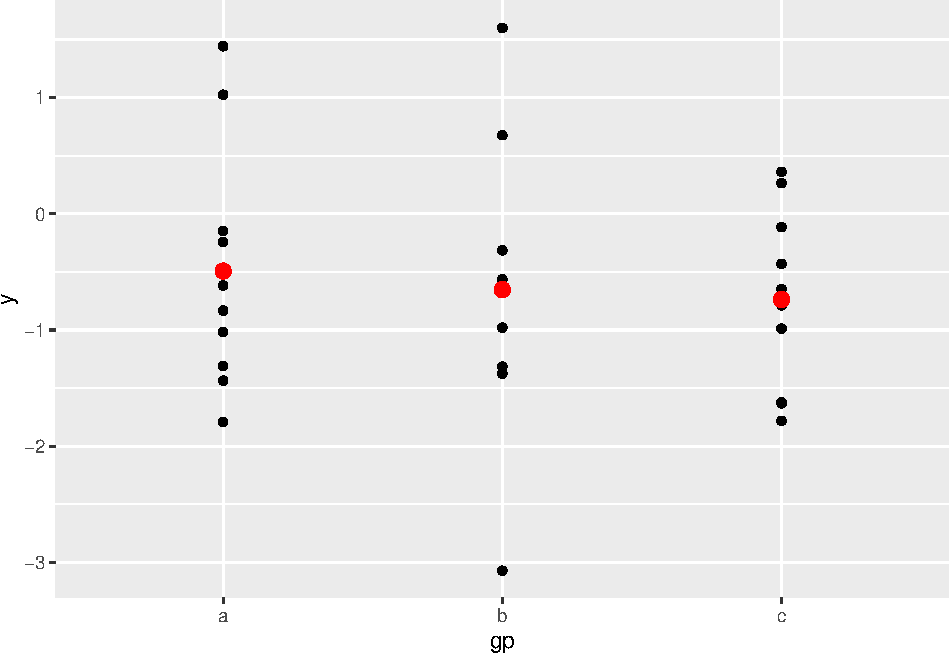
\includegraphics{02-literature_files/figure-latex/ggplot02-1.pdf}

\begin{enumerate}
\def\labelenumi{\arabic{enumi}.}
\setcounter{enumi}{5}
\tightlist
\item
  漂亮图形的几大要素:

  \begin{itemize}
  \tightlist
  \item
    数据类型(Data Component): 不同的数据类型使用合适的图形来表示,条形图(离散型数据)、直方图(连续型数据)等。
  \item
    几何要素(Geometric Component): 根据数据选择合适的的图形scatter plot, line graphs, barplots, histograms, qqplots, smooth densities, boxplots, pairplots, heatmaps, etc.
  \item
    坐标要素(Mapping Component): 选择合适的横坐标和纵坐标.
  \item
    刻度要素(Scale Component):选择合适的刻度. linear scale, log scale, etc.
  \item
    标识要素(Labels Component): This include things like axes labels, titles, legends, font size to use, etc.
  \item
    Ethical Component: Here, you want to make sure your visualization tells the true story. You need to be aware of your actions when cleaning, summarizing, manipulating and producing a data visualization and ensure you aren't using your visualization to mislead or manipulate your audience.
  \end{itemize}
\end{enumerate}

\hypertarget{ux6570ux636eux6574ux7406ux548cux6e05ux7406}{%
\chapter{数据整理和清理}\label{ux6570ux636eux6574ux7406ux548cux6e05ux7406}}

\begin{itemize}
\item
  从各种不同来源得到的数据可能存在数据的格式混乱、数据冗余(重复)、含缺失值(missing data)、异常值(outlier)等问题,无法直接用于模型构建,所以建模的第一步就是完成数据清洗和重构。
\item
  数据科学家日常的工作大约有80\%的时间都用于清洗数据。
\end{itemize}

\hypertarget{ux6570ux636eux7684ux7b5bux9009}{%
\section{数据的筛选}\label{ux6570ux636eux7684ux7b5bux9009}}

\begin{itemize}
\tightlist
\item
  选出符合条件的数据:根据一定的条件筛选出符合条件的数据子集;
\end{itemize}

\begin{Shaded}
\begin{Highlighting}[]
\CommentTok{\# download data from http://data.un.org/Data.aspx?q=GDP\&d=SNAAMA\&f=grID\%3a101\%3bcurrID\%3aNCU\%3bpcFlag\%3a0}
\FunctionTok{library}\NormalTok{(tidyverse)}
\end{Highlighting}
\end{Shaded}

\begin{verbatim}
## -- Attaching packages --------------------------------------- tidyverse 1.3.1 --
\end{verbatim}

\begin{verbatim}
## v ggplot2 3.3.5     v purrr   0.3.4
## v tibble  3.1.6     v dplyr   1.0.8
## v tidyr   1.2.0     v stringr 1.4.0
## v readr   2.1.2     v forcats 0.5.1
\end{verbatim}

\begin{verbatim}
## -- Conflicts ------------------------------------------ tidyverse_conflicts() --
## x dplyr::filter() masks stats::filter()
## x dplyr::lag()    masks stats::lag()
\end{verbatim}

\begin{Shaded}
\begin{Highlighting}[]
\FunctionTok{library}\NormalTok{(ggplot2)}

\NormalTok{gdp1 }\OtherTok{\textless{}{-}} \FunctionTok{read.csv}\NormalTok{(}\StringTok{"./data/UNdata\_Export\_20220406\_093714228.csv"}\NormalTok{)}

\FunctionTok{head}\NormalTok{(gdp1)}
\end{Highlighting}
\end{Shaded}

\begin{verbatim}
##   Country.or.Area Year
## 1     Afghanistan 2020
## 2     Afghanistan 2020
## 3     Afghanistan 2020
## 4     Afghanistan 2020
## 5     Afghanistan 2020
## 6     Afghanistan 2020
##                                                                                       Item
## 1                                                            Final consumption expenditure
## 2 Household consumption expenditure (including Non-profit institutions serving households)
## 3                                         General government final consumption expenditure
## 4                                                                  Gross capital formation
## 5       Gross fixed capital formation (including Acquisitions less disposals of valuables)
## 6                                                            Exports of goods and services
##          Value
## 1 1.628089e+12
## 2 1.354293e+12
## 3 2.737961e+11
## 4 1.816860e+11
## 5 1.816860e+11
## 6 2.043364e+11
\end{verbatim}

\begin{Shaded}
\begin{Highlighting}[]
\FunctionTok{names}\NormalTok{(gdp1)}
\end{Highlighting}
\end{Shaded}

\begin{verbatim}
## [1] "Country.or.Area" "Year"            "Item"            "Value"
\end{verbatim}

\begin{Shaded}
\begin{Highlighting}[]
\CommentTok{\#levels(as.factor(gdp1[,3]))=paste0("V",1:9)}
\NormalTok{tb }\OtherTok{\textless{}{-}} \FunctionTok{as.tibble}\NormalTok{(gdp1)}
\end{Highlighting}
\end{Shaded}

\begin{verbatim}
## Warning: `as.tibble()` was deprecated in tibble 2.0.0.
## Please use `as_tibble()` instead.
## The signature and semantics have changed, see `?as_tibble`.
## This warning is displayed once every 8 hours.
## Call `lifecycle::last_lifecycle_warnings()` to see where this warning was generated.
\end{verbatim}

\begin{Shaded}
\begin{Highlighting}[]
\FunctionTok{head}\NormalTok{(tb)}
\end{Highlighting}
\end{Shaded}

\begin{verbatim}
## # A tibble: 6 x 4
##   Country.or.Area  Year Item                                               Value
##   <chr>           <int> <chr>                                              <dbl>
## 1 Afghanistan      2020 Final consumption expenditure                    1.63e12
## 2 Afghanistan      2020 Household consumption expenditure (including No~ 1.35e12
## 3 Afghanistan      2020 General government final consumption expenditure 2.74e11
## 4 Afghanistan      2020 Gross capital formation                          1.82e11
## 5 Afghanistan      2020 Gross fixed capital formation (including Acquis~ 1.82e11
## 6 Afghanistan      2020 Exports of goods and services                    2.04e11
\end{verbatim}

\begin{Shaded}
\begin{Highlighting}[]
\FunctionTok{names}\NormalTok{(tb)}
\end{Highlighting}
\end{Shaded}

\begin{verbatim}
## [1] "Country.or.Area" "Year"            "Item"            "Value"
\end{verbatim}

\begin{Shaded}
\begin{Highlighting}[]
\CommentTok{\# filter year 2016 data}
\NormalTok{tb2016 }\OtherTok{\textless{}{-}}\NormalTok{ tb[tb}\SpecialCharTok{$}\NormalTok{Year}\SpecialCharTok{==}\DecValTok{2016}\NormalTok{,}\SpecialCharTok{{-}}\DecValTok{2}\NormalTok{]}\SpecialCharTok{\%\textgreater{}\%}\FunctionTok{spread}\NormalTok{(}\AttributeTok{key=}\StringTok{"Item"}\NormalTok{,}\AttributeTok{value=}\StringTok{"Value"}\NormalTok{)}
\FunctionTok{head}\NormalTok{(tb2016,}\DecValTok{3}\NormalTok{)}
\end{Highlighting}
\end{Shaded}

\begin{verbatim}
## # A tibble: 3 x 10
##   Country.or.Area `Changes in inventories` `Exports of goods ~` `Final consump~`
##   <chr>                              <dbl>                <dbl>            <dbl>
## 1 Afghanistan                           NA         203769211430          1.26e12
## 2 Albania                      12602872911         426693482069          1.36e12
## 3 Algeria                    1349202900000        3655739600000          1.11e13
## # ... with 6 more variables:
## #   `General government final consumption expenditure` <dbl>,
## #   `Gross capital formation` <dbl>, `Gross Domestic Product (GDP)` <dbl>,
## #   `Gross fixed capital formation (including Acquisitions less disposals of valuables)` <dbl>,
## #   `Household consumption expenditure (including Non-profit institutions serving households)` <dbl>,
## #   `Imports of goods and services` <dbl>
\end{verbatim}

\begin{Shaded}
\begin{Highlighting}[]
\FunctionTok{names}\NormalTok{(tb2016)[}\DecValTok{2}\SpecialCharTok{:}\DecValTok{10}\NormalTok{] }\OtherTok{\textless{}{-}} \FunctionTok{paste0}\NormalTok{(}\StringTok{"V"}\NormalTok{,}\DecValTok{1}\SpecialCharTok{:}\DecValTok{9}\NormalTok{)}
\FunctionTok{head}\NormalTok{(tb2016)}
\end{Highlighting}
\end{Shaded}

\begin{verbatim}
## # A tibble: 6 x 10
##   Country.or.Area            V1       V2      V3      V4      V5      V6      V7
##   <chr>                   <dbl>    <dbl>   <dbl>   <dbl>   <dbl>   <dbl>   <dbl>
## 1 Afghanistan                NA  2.04e11 1.26e12 2.81e11 1.54e11 1.22e12 1.54e11
## 2 Albania           12602872911  4.27e11 1.36e12 1.66e11 3.71e11 1.47e12 3.59e11
## 3 Algeria         1349202900000  3.66e12 1.11e13 3.66e12 8.89e12 1.75e13 7.54e12
## 4 Andorra              20754648  8.87e 8 2.02e 9 4.99e 8 4.91e 8 2.62e 9 4.70e 8
## 5 Angola           165743151505  4.65e12 1.16e13 2.30e12 4.50e12 1.65e13 4.34e12
## 6 Anguilla                   NA  5.62e 8 8.62e 8 1.41e 8 1.80e 8 8.61e 8 1.80e 8
## # ... with 2 more variables: V8 <dbl>, V9 <dbl>
\end{verbatim}

\begin{Shaded}
\begin{Highlighting}[]
\FunctionTok{ggplot}\NormalTok{(tb2016,}\FunctionTok{aes}\NormalTok{(}\AttributeTok{x=}\NormalTok{V4,}\AttributeTok{y=}\NormalTok{V5))}\SpecialCharTok{+}
  \FunctionTok{geom\_point}\NormalTok{()}\SpecialCharTok{+}
  \FunctionTok{geom\_smooth}\NormalTok{()}
\end{Highlighting}
\end{Shaded}

\begin{verbatim}
## `geom_smooth()` using method = 'loess' and formula 'y ~ x'
\end{verbatim}

\begin{verbatim}
## Warning: Removed 1 rows containing non-finite values (stat_smooth).
\end{verbatim}

\begin{verbatim}
## Warning: Removed 1 rows containing missing values (geom_point).
\end{verbatim}

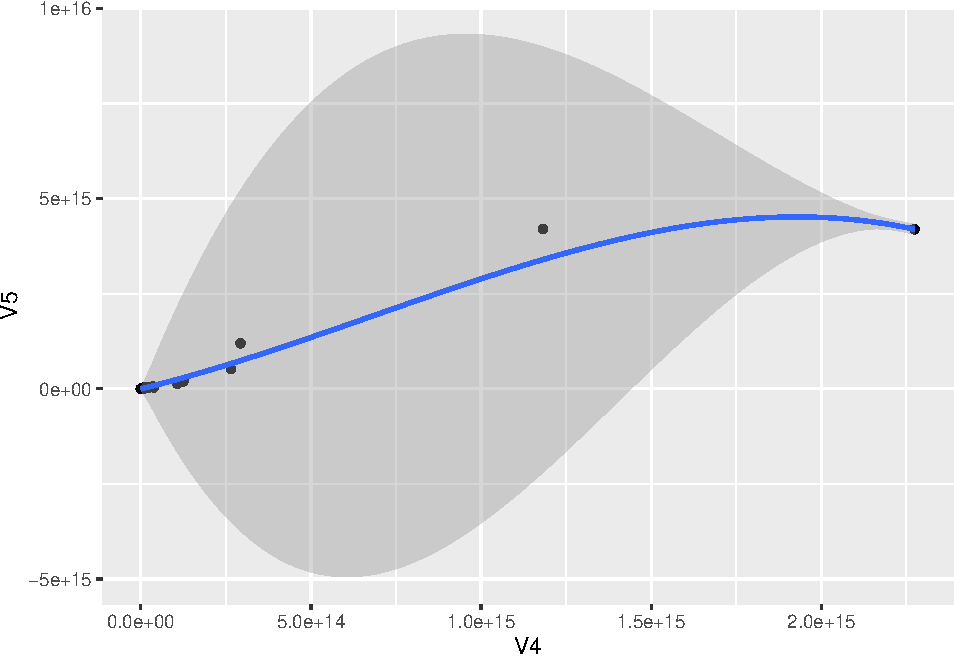
\includegraphics{03-method_files/figure-latex/datacleaning-1.pdf}

\begin{Shaded}
\begin{Highlighting}[]
\CommentTok{\# Draw time series chart}
\NormalTok{tb }\SpecialCharTok{\%\textgreater{}\%} \FunctionTok{subset}\NormalTok{(Country.or.Area}\SpecialCharTok{==}\StringTok{"Japan"}\NormalTok{) }\SpecialCharTok{\%\textgreater{}\%}
  \FunctionTok{ggplot}\NormalTok{(}\FunctionTok{aes}\NormalTok{(}\AttributeTok{x=}\NormalTok{Year,}\AttributeTok{y=}\NormalTok{Value))}\SpecialCharTok{+}
    \FunctionTok{geom\_line}\NormalTok{(}\FunctionTok{aes}\NormalTok{(}\AttributeTok{color=}\NormalTok{Item),}\AttributeTok{size=}\DecValTok{1}\NormalTok{)}\SpecialCharTok{+}
    \FunctionTok{theme\_minimal}\NormalTok{()}
\end{Highlighting}
\end{Shaded}

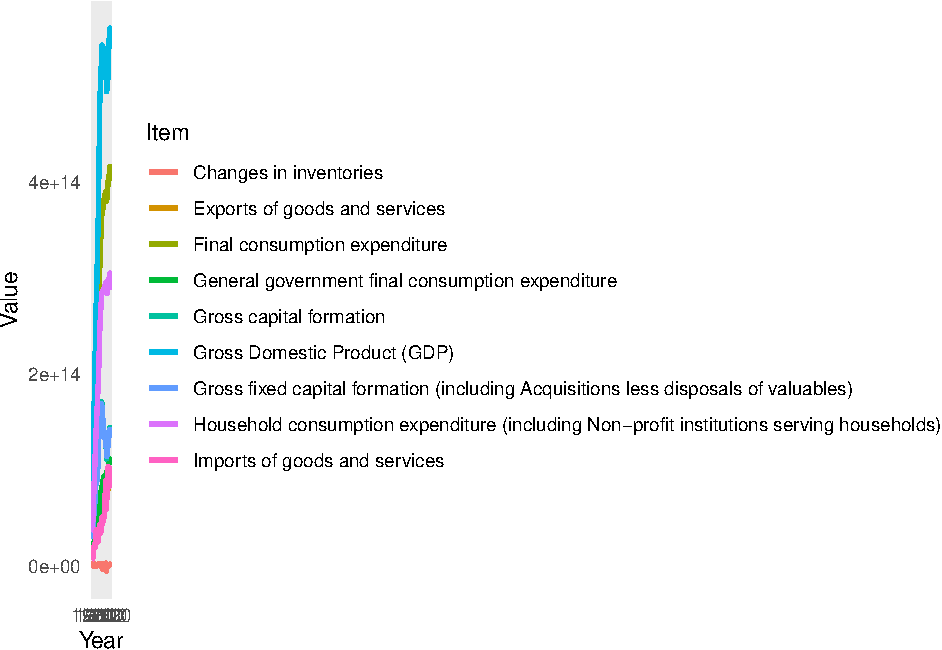
\includegraphics{03-method_files/figure-latex/datacleaning-2.pdf}

\hypertarget{ux6570ux636eux5408ux5e76}{%
\section{数据合并}\label{ux6570ux636eux5408ux5e76}}

\begin{itemize}
\tightlist
\item
  把多个数据合并在一起;
\end{itemize}

\begin{Shaded}
\begin{Highlighting}[]
\NormalTok{NN }\OtherTok{\textless{}{-}}  \FunctionTok{c}\NormalTok{(}\StringTok{"./data/D1.csv"}\NormalTok{,}\StringTok{"./data/D2.csv"}\NormalTok{,}\StringTok{"./data/D3.csv"}\NormalTok{)}
\NormalTok{df }\OtherTok{\textless{}{-}} \FunctionTok{lapply}\NormalTok{(NN,read.csv)}
\FunctionTok{head}\NormalTok{(df)}
\end{Highlighting}
\end{Shaded}

\begin{verbatim}
## [[1]]
##                               Country.or.Area Year.s. Value Value.Footnotes
## 1                                 Afghanistan    2012  -2.4              NA
## 2                                     Albania    2012  -0.3              NA
## 3                                     Algeria    2012  -1.9              NA
## 4                                     Andorra    2012   0.0              NA
## 5                                      Angola    2012  -3.1              NA
## 6                         Antigua and Barbuda    2012  -1.1              NA
## 7                                   Argentina    2012  -0.9              NA
## 8                                     Armenia    2012  -0.2              NA
## 9                                   Australia    2012  -1.3              NA
## 10                                    Austria    2012  -0.4              NA
## 11                                 Azerbaijan    2012  -1.2              NA
## 12                                    Bahamas    2012  -1.6              NA
## 13                                    Bahrain    2012  -1.9              NA
## 14                                 Bangladesh    2012  -1.3              NA
## 15                                   Barbados    2012  -0.4              NA
## 16                                    Belarus    2012   0.5              NA
## 17                                    Belgium    2012  -0.5              NA
## 18                                     Belize    2012  -2.5              NA
## 19                                      Benin    2012  -2.7              NA
## 20                                     Bhutan    2012  -1.8              NA
## 21           Bolivia (Plurinational State of)    2012  -1.7              NA
## 22                     Bosnia and Herzegovina    2012   0.1              NA
## 23                                   Botswana    2012  -0.9              NA
## 24                                     Brazil    2012  -1.0              NA
## 25                          Brunei Darussalam    2012  -1.2              NA
## 26                                   Bulgaria    2012   0.8              NA
## 27                               Burkina Faso    2012  -2.9              NA
## 28                                    Burundi    2012  -3.2              NA
## 29                                 Cabo Verde    2012  -0.6              NA
## 30                                   Cambodia    2012  -1.8              NA
## 31                                   Cameroon    2012  -2.5              NA
## 32                                     Canada    2012  -1.0              NA
## 33                   Central African Republic    2012  -2.0              NA
## 34                                       Chad    2012  -3.0              NA
## 35                                      Chile    2012  -0.9              NA
## 36                                      China    2012  -0.7              NA
## 37                                   Colombia    2012  -1.3              NA
## 38                                    Comoros    2012  -2.5              NA
## 39                                      Congo    2012  -2.6              NA
## 40                               Cook Islands    2012  -4.9              NA
## 41                                 Costa Rica    2012  -1.4              NA
## 42                              Côte d’Ivoire    2012  -2.3              NA
## 43                                    Croatia    2012   0.4              NA
## 44                                       Cuba    2012   0.0              NA
## 45                                     Cyprus    2012  -1.1              NA
## 46                             Czech Republic    2012  -0.5              NA
## 47      Democratic People's Republic of Korea    2012  -0.5              NA
## 48           Democratic Republic of the Congo    2012  -2.7              NA
## 49                                    Denmark    2012  -0.4              NA
## 50                                   Djibouti    2012  -1.5              NA
## 51                                   Dominica    2012  -1.4              NA
## 52                         Dominican Republic    2012  -1.3              NA
## 53                                    Ecuador    2012  -1.6              NA
## 54                                      Egypt    2012  -1.7              NA
## 55                                El Salvador    2012  -0.7              NA
## 56                          Equatorial Guinea    2012  -2.8              NA
## 57                                    Eritrea    2012  -3.3              NA
## 58                                    Estonia    2012   0.2              NA
## 59                                   Ethiopia    2012  -2.6              NA
## 60                                       Fiji    2012  -0.8              NA
## 61                                    Finland    2012  -0.4              NA
## 62                                     France    2012  -0.6              NA
## 63                                      Gabon    2012  -2.4              NA
## 64                                     Gambia    2012  -3.2              NA
## 65                                    Georgia    2012   0.4              NA
## 66                                    Germany    2012   0.1              NA
## 67                                      Ghana    2012  -2.2              NA
## 68                                     Greece    2012  -0.1              NA
## 69                                    Grenada    2012   0.0              NA
## 70                                  Guatemala    2012  -2.5              NA
## 71                                     Guinea    2012  -2.6              NA
## 72                              Guinea-Bissau    2012  -2.4              NA
## 73                                     Guyana    2012  -0.5              NA
## 74                                      Haiti    2012  -1.4              NA
## 75                                   Honduras    2012  -2.0              NA
## 76                                    Hungary    2012   0.2              NA
## 77                                    Iceland    2012  -1.2              NA
## 78                                      India    2012  -1.6              NA
## 79                                  Indonesia    2012  -1.2              NA
## 80                 Iran (Islamic Republic of)    2012  -1.3              NA
## 81                                       Iraq    2012  -2.9              NA
## 82                                    Ireland    2012  -1.2              NA
## 83                                     Israel    2012  -1.3              NA
## 84                                      Italy    2012  -0.3              NA
## 85                                    Jamaica    2012  -0.5              NA
## 86                                      Japan    2012   0.0              NA
## 87                                     Jordan    2012  -4.0              NA
## 88                                 Kazakhstan    2012  -1.1              NA
## 89                                      Kenya    2012  -2.7              NA
## 90                                   Kiribati    2012  -2.0              NA
## 91                                     Kuwait    2012  -3.9              NA
## 92                                 Kyrgyzstan    2012  -1.3              NA
## 93           Lao People's Democratic Republic    2012  -1.9              NA
## 94                                     Latvia    2012   0.6              NA
## 95                                    Lebanon    2012  -3.7              NA
## 96                                    Lesotho    2012  -1.1              NA
## 97                                    Liberia    2012  -2.7              NA
## 98                                      Libya    2012  -0.8              NA
## 99                                  Lithuania    2012   0.5              NA
## 100                                Luxembourg    2012  -1.5              NA
## 101                                Madagascar    2012  -2.8              NA
## 102                                    Malawi    2012  -2.9              NA
## 103                                  Malaysia    2012  -1.7              NA
## 104                                  Maldives    2012  -1.8              NA
## 105                                      Mali    2012  -3.0              NA
## 106                                     Malta    2012  -0.5              NA
## 107                          Marshall Islands    2012  -1.9              NA
## 108                                Mauritania    2012  -2.5              NA
## 109                                 Mauritius    2012  -0.4              NA
## 110                                    Mexico    2012  -1.7              NA
## 111          Micronesia (Federated States of)    2012   0.0              NA
## 112                                    Monaco    2012  -2.7              NA
## 113                                  Mongolia    2012  -1.5              NA
## 114                                Montenegro    2012   0.0              NA
## 115                                   Morocco    2012  -1.4              NA
## 116                                Mozambique    2012  -2.5              NA
## 117                                   Myanmar    2012  -0.8              NA
## 118                                   Namibia    2012  -1.8              NA
## 119                                     Nauru    2012   0.0              NA
## 120                                     Nepal    2012  -1.2              NA
## 121                               Netherlands    2012  -0.3              NA
## 122                               New Zealand    2012  -1.0              NA
## 123                                 Nicaragua    2012  -1.5              NA
## 124                                     Niger    2012  -3.8              NA
## 125                                   Nigeria    2012  -3.0              NA
## 126                                      Niue    2012   0.0              NA
## 127                                    Norway    2012  -1.0              NA
## 128                                      Oman    2012  -9.1              NA
## 129                                  Pakistan    2012  -1.7              NA
## 130                                     Palau    2012   0.0              NA
## 131                                    Panama    2012  -1.6              NA
## 132                          Papua New Guinea    2012  -2.2              NA
## 133                                  Paraguay    2012  -1.7              NA
## 134                                      Peru    2012  -1.3              NA
## 135                               Philippines    2012  -1.7              NA
## 136                                    Poland    2012   0.0              NA
## 137                                  Portugal    2012  -0.1              NA
## 138                                     Qatar    2012  -7.1              NA
## 139                         Republic of Korea    2012  -0.6              NA
## 140                       Republic of Moldova    2012   0.8              NA
## 141                                   Romania    2012   0.2              NA
## 142                        Russian Federation    2012   0.0              NA
## 143                                    Rwanda    2012  -2.8              NA
## 144                     Saint Kitts and Nevis    2012  -1.9              NA
## 145                               Saint Lucia    2012  -1.1              NA
## 146          Saint Vincent and the Grenadines    2012   0.0              NA
## 147                                     Samoa    2012  -1.1              NA
## 148                                San Marino    2012   0.0              NA
## 149                     Sao Tome and Principe    2012  -2.7              NA
## 150                              Saudi Arabia    2012  -1.9              NA
## 151                                   Senegal    2012  -2.9              NA
## 152                                    Serbia    2012   0.5              NA
## 153                                Seychelles    2012   0.0              NA
## 154                              Sierra Leone    2012  -1.9              NA
## 155                                 Singapore    2012  -2.1              NA
## 156                                  Slovakia    2012  -0.1              NA
## 157                                  Slovenia    2012  -0.3              NA
## 158                           Solomon Islands    2012  -2.2              NA
## 159                                   Somalia    2012  -2.9              NA
## 160                              South Africa    2012  -0.8              NA
## 161                               South Sudan    2012  -4.3              NA
## 162                                     Spain    2012  -0.5              NA
## 163                                 Sri Lanka    2012  -0.8              NA
## 164                                     Sudan    2012  -2.1              NA
## 165                                  Suriname    2012  -0.9              NA
## 166                                 Swaziland    2012  -1.6              NA
## 167                                    Sweden    2012  -0.7              NA
## 168                               Switzerland    2012  -1.0              NA
## 169                      Syrian Arab Republic    2012  -0.4              NA
## 170                                Tajikistan    2012  -2.5              NA
## 171                                  Thailand    2012  -0.3              NA
## 172 The former Yugoslav Republic of Macedonia    2012  -0.1              NA
## 173                               Timor-Leste    2012  -1.6              NA
## 174                                      Togo    2012  -2.6              NA
## 175                                     Tonga    2012   0.0              NA
## 176                       Trinidad and Tobago    2012  -0.3              NA
## 177                                   Tunisia    2012  -1.1              NA
## 178                                    Turkey    2012  -1.3              NA
## 179                              Turkmenistan    2012  -1.3              NA
## 180                                    Tuvalu    2012   0.0              NA
## 181                                    Uganda    2012  -3.4              NA
## 182                                   Ukraine    2012   0.6              NA
## 183                      United Arab Emirates    2012  -3.1              NA
## 184                            United Kingdom    2012  -0.6              NA
## 185               United Republic of Tanzania    2012  -3.0              NA
## 186                  United States of America    2012  -0.9              NA
## 187                                   Uruguay    2012  -0.4              NA
## 188                                Uzbekistan    2012  -1.4              NA
## 189                                   Vanuatu    2012  -2.0              NA
## 190        Venezuela (Bolivarian Republic of)    2012  -1.5              NA
## 191                                  Viet Nam    2012  -1.0              NA
## 192                                     Yemen    2012  -2.3              NA
## 193                                    Zambia    2012  -3.2              NA
## 194                                  Zimbabwe    2012  -2.7              NA
## 
## [[2]]
##                               Country.or.Area Year.s. Value Value.Footnotes
## 1                                 Afghanistan    2012    60              NA
## 2                                 Afghanistan    2011    54              NA
## 3                                 Afghanistan    2010    41              NA
## 4                                     Albania    2012   111              NA
## 5                                     Albania    2011    96              NA
## 6                                     Albania    2010   142              NA
## 7                                     Algeria    2012    98              NA
## 8                                     Algeria    2011    99              NA
## 9                                     Algeria    2010    92              NA
## 10                                    Andorra    2012    81              NA
## 11                                    Andorra    2011    75              NA
## 12                                    Andorra    2010    77              NA
## 13                                     Angola    2012    47              NA
## 14                                     Angola    2011    48              NA
## 15                                     Angola    2010    47              NA
## 16                        Antigua and Barbuda    2012   143              NA
## 17                        Antigua and Barbuda    2011   196              NA
## 18                        Antigua and Barbuda    2010   189              NA
## 19                                  Argentina    2012   152              NA
## 20                                  Argentina    2011   135              NA
## 21                                  Argentina    2010   142              NA
## 22                                    Armenia    2012   112              NA
## 23                                    Armenia    2011   104              NA
## 24                                    Armenia    2010   125              NA
## 25                                  Australia    2012   106              NA
## 26                                  Australia    2011   108              NA
## 27                                  Australia    2010   101              NA
## 28                                    Austria    2012   161              NA
## 29                                    Austria    2011   155              NA
## 30                                    Austria    2010   146              NA
## 31                                 Azerbaijan    2012   109              NA
## 32                                 Azerbaijan    2011   109              NA
## 33                                 Azerbaijan    2010    99              NA
## 34                                    Bahamas    2012    81              NA
## 35                                    Bahamas    2011    86              NA
## 36                                    Bahamas    2010   125              NA
## 37                                    Bahrain    2012   161              NA
## 38                                    Bahrain    2011   128              NA
## 39                                    Bahrain    2010   124              NA
## 40                                 Bangladesh    2012    63              NA
## 41                                 Bangladesh    2011    56              NA
## 42                                 Bangladesh    2010    46              NA
## 43                                   Barbados    2012   123              NA
## 44                                   Barbados    2011   127              NA
## 45                                   Barbados    2010   128              NA
## 46                                    Belarus    2012   114              NA
## 47                                    Belarus    2011   112              NA
## 48                                    Belarus    2010   108              NA
## 49                                    Belgium    2012   111              NA
## 50                                    Belgium    2011   117              NA
## 51                                    Belgium    2010   113              NA
## 52                                     Belize    2012    53              NA
## 53                                     Belize    2011    70              NA
## 54                                     Belize    2010    62              NA
## 55                                      Benin    2012    84              NA
## 56                                      Benin    2011    85              NA
## 57                                      Benin    2010    80              NA
## 58                                     Bhutan    2012    76              NA
## 59                                     Bhutan    2011    66              NA
## 60                                     Bhutan    2010    54              NA
## 61           Bolivia (Plurinational State of)    2012    90              NA
## 62           Bolivia (Plurinational State of)    2011    83              NA
## 63           Bolivia (Plurinational State of)    2010    72              NA
## 64                     Bosnia and Herzegovina    2012    88              NA
## 65                     Bosnia and Herzegovina    2011    85              NA
## 66                     Bosnia and Herzegovina    2010    83              NA
## 67                                   Botswana    2012   154              NA
## 68                                   Botswana    2011   143              NA
## 69                                   Botswana    2010   118              NA
## 70                                     Brazil    2012   125              NA
## 71                                     Brazil    2011   124              NA
## 72                                     Brazil    2010   104              NA
## 73                          Brunei Darussalam    2012   114              NA
## 74                          Brunei Darussalam    2011   109              NA
## 75                          Brunei Darussalam    2010   109              NA
## 76                                   Bulgaria    2012   148              NA
## 77                                   Bulgaria    2011   141              NA
## 78                                   Bulgaria    2010   136              NA
## 79                               Burkina Faso    2012    61              NA
## 80                               Burkina Faso    2011    45              NA
## 81                               Burkina Faso    2010    35              NA
## 82                                    Burundi    2012    23              NA
## 83                                    Burundi    2011    22              NA
## 84                                    Burundi    2010    14              NA
## 85                                 Cabo Verde    2012    86              NA
## 86                                 Cabo Verde    2011    79              NA
## 87                                 Cabo Verde    2010    75              NA
## 88                                   Cambodia    2012   129              NA
## 89                                   Cambodia    2011    96              NA
## 90                                   Cambodia    2010    58              NA
## 91                                   Cameroon    2012    60              NA
## 92                                   Cameroon    2011    52              NA
## 93                                   Cameroon    2010    44              NA
## 94                                     Canada    2012    80              NA
## 95                                     Canada    2011    80              NA
## 96                                     Canada    2010    71              NA
## 97                   Central African Republic    2012    25              NA
## 98                   Central African Republic    2011    41              NA
## 99                   Central African Republic    2010    22              NA
## 100                                      Chad    2012    35              NA
## 101                                      Chad    2011    32              NA
## 102                                      Chad    2010    24              NA
## 103                                     Chile    2012   138              NA
## 104                                     Chile    2011   130              NA
## 105                                     Chile    2010   116              NA
## 106                                     China    2012    80              NA
## 107                                     China    2011    73              NA
## 108                                     China    2010    64              NA
## 109                                  Colombia    2012   103              NA
## 110                                  Colombia    2011    98              NA
## 111                                  Colombia    2010    96              NA
## 112                                   Comoros    2012    40              NA
## 113                                   Comoros    2011    29              NA
## 114                                   Comoros    2010    22              NA
## 115                                     Congo    2012    99              NA
## 116                                     Congo    2011    94              NA
## 117                                     Congo    2010    94              NA
## 118                              Cook Islands    2010    38              NA
## 119                                Costa Rica    2012   112              NA
## 120                                Costa Rica    2011    92              NA
## 121                                Costa Rica    2010    65              NA
## 122                             Côte d’Ivoire    2012    91              NA
## 123                             Côte d’Ivoire    2011    86              NA
## 124                             Côte d’Ivoire    2010    76              NA
## 125                                   Croatia    2012   115              NA
## 126                                   Croatia    2011   116              NA
## 127                                   Croatia    2010   144              NA
## 128                                      Cuba    2012    15              NA
## 129                                      Cuba    2011    12              NA
## 130                                      Cuba    2010     9              NA
## 131                                    Cyprus    2012    98              NA
## 132                                    Cyprus    2011    98              NA
## 133                                    Cyprus    2010    94              NA
## 134                            Czech Republic    2012   127              NA
## 135                            Czech Republic    2011   123              NA
## 136                            Czech Republic    2010   137              NA
## 137     Democratic People's Republic of Korea    2012     7              NA
## 138     Democratic People's Republic of Korea    2011     4              NA
## 139     Democratic People's Republic of Korea    2010     2              NA
## 140          Democratic Republic of the Congo    2012    31              NA
## 141          Democratic Republic of the Congo    2011    23              NA
## 142          Democratic Republic of the Congo    2010    18              NA
## 143                                   Denmark    2012   118              NA
## 144                                   Denmark    2011   128              NA
## 145                                   Denmark    2010   125              NA
## 146                                  Djibouti    2012    25              NA
## 147                                  Djibouti    2011    21              NA
## 148                                  Djibouti    2010    19              NA
## 149                                  Dominica    2012   152              NA
## 150                                  Dominica    2011   164              NA
## 151                                  Dominica    2010   156              NA
## 152                        Dominican Republic    2012    87              NA
## 153                        Dominican Republic    2011    87              NA
## 154                        Dominican Republic    2010    90              NA
## 155                                   Ecuador    2012   106              NA
## 156                                   Ecuador    2011   105              NA
## 157                                   Ecuador    2010   102              NA
## 158                                     Egypt    2012   120              NA
## 159                                     Egypt    2011   101              NA
## 160                                     Egypt    2010    87              NA
## 161                               El Salvador    2012   137              NA
## 162                               El Salvador    2011   134              NA
## 163                               El Salvador    2010   124              NA
## 164                         Equatorial Guinea    2012    68              NA
## 165                         Equatorial Guinea    2011    59              NA
## 166                         Equatorial Guinea    2010    57              NA
## 167                                   Eritrea    2012     5              NA
## 168                                   Eritrea    2011     4              NA
## 169                                   Eritrea    2010     4              NA
## 170                                   Estonia    2012   160              NA
## 171                                   Estonia    2011   139              NA
## 172                                   Estonia    2010   123              NA
## 173                                  Ethiopia    2012    22              NA
## 174                                  Ethiopia    2011    17              NA
## 175                                  Ethiopia    2010     8              NA
## 176                                      Fiji    2012    98              NA
## 177                                      Fiji    2011    84              NA
## 178                                      Fiji    2010    81              NA
## 179                                   Finland    2012   172              NA
## 180                                   Finland    2011   166              NA
## 181                                   Finland    2010   156              NA
## 182                                    France    2012    97              NA
## 183                                    France    2011    95              NA
## 184                                    France    2010   101              NA
## 185                                     Gabon    2012   179              NA
## 186                                     Gabon    2011   117              NA
## 187                                     Gabon    2010   107              NA
## 188                                    Gambia    2012    85              NA
## 189                                    Gambia    2011    79              NA
## 190                                    Gambia    2010    86              NA
## 191                                   Georgia    2012   108              NA
## 192                                   Georgia    2011   102              NA
## 193                                   Georgia    2010    91              NA
## 194                                   Germany    2012   112              NA
## 195                                   Germany    2011   132              NA
## 196                                   Germany    2010   127              NA
## 197                                     Ghana    2012   101              NA
## 198                                     Ghana    2011    85              NA
## 199                                     Ghana    2010    71              NA
## 200                                    Greece    2012   120              NA
## 201                                    Greece    2011   106              NA
## 202                                    Greece    2010   108              NA
## 203                                   Grenada    2012   121              NA
## 204                                   Grenada    2010   117              NA
## 205                                 Guatemala    2012   138              NA
## 206                                 Guatemala    2011   140              NA
## 207                                 Guatemala    2010   126              NA
## 208                                    Guinea    2012    42              NA
## 209                                    Guinea    2011    44              NA
## 210                                    Guinea    2010    40              NA
## 211                             Guinea-Bissau    2012    63              NA
## 212                             Guinea-Bissau    2011    56              NA
## 213                             Guinea-Bissau    2010    39              NA
## 214                                    Guyana    2012    69              NA
## 215                                    Guyana    2011    70              NA
## 216                                    Guyana    2010    74              NA
## 217                                     Haiti    2012    60              NA
## 218                                     Haiti    2011    41              NA
## 219                                     Haiti    2010    40              NA
## 220                                  Honduras    2012    93              NA
## 221                                  Honduras    2011   104              NA
## 222                                  Honduras    2010   125              NA
## 223                                   Hungary    2012   116              NA
## 224                                   Hungary    2011   117              NA
## 225                                   Hungary    2010   120              NA
## 226                                   Iceland    2012   108              NA
## 227                                   Iceland    2011   106              NA
## 228                                   Iceland    2010   107              NA
## 229                                     India    2012    70              NA
## 230                                     India    2011    72              NA
## 231                                     India    2010    61              NA
## 232                                 Indonesia    2012   114              NA
## 233                                 Indonesia    2011   103              NA
## 234                                 Indonesia    2010    92              NA
## 235                Iran (Islamic Republic of)    2012    76              NA
## 236                Iran (Islamic Republic of)    2011    75              NA
## 237                Iran (Islamic Republic of)    2010    91              NA
## 238                                      Iraq    2012    82              NA
## 239                                      Iraq    2011    78              NA
## 240                                      Iraq    2010    76              NA
## 241                                   Ireland    2012   107              NA
## 242                                   Ireland    2011   108              NA
## 243                                   Ireland    2010   105              NA
## 244                                    Israel    2012   121              NA
## 245                                    Israel    2011   122              NA
## 246                                    Israel    2010   133              NA
## 247                                     Italy    2012   160              NA
## 248                                     Italy    2011   158              NA
## 249                                     Italy    2010   150              NA
## 250                                   Jamaica    2012    96              NA
## 251                                   Jamaica    2011   108              NA
## 252                                   Jamaica    2010   116              NA
## 253                                     Japan    2012   111              NA
## 254                                     Japan    2011   105              NA
## 255                                     Japan    2010    95              NA
## 256                                    Jordan    2012   128              NA
## 257                                    Jordan    2011   118              NA
## 258                                    Jordan    2010   107              NA
## 259                                Kazakhstan    2012   186              NA
## 260                                Kazakhstan    2011   156              NA
## 261                                Kazakhstan    2010   121              NA
## 262                                     Kenya    2012    71              NA
## 263                                     Kenya    2011    67              NA
## 264                                     Kenya    2010    62              NA
## 265                                  Kiribati    2012    16              NA
## 266                                  Kiribati    2011    14              NA
## 267                                  Kiribati    2010    10              NA
## 268                                    Kuwait    2012   157              NA
## 269                                    Kuwait    2011   175              NA
## 270                                    Kuwait    2010   161              NA
## 271                                Kyrgyzstan    2012   124              NA
## 272                                Kyrgyzstan    2011   116              NA
## 273                                Kyrgyzstan    2010    99              NA
## 274          Lao People's Democratic Republic    2012    65              NA
## 275          Lao People's Democratic Republic    2011    87              NA
## 276          Lao People's Democratic Republic    2010    65              NA
## 277                                    Latvia    2012   112              NA
## 278                                    Latvia    2011   103              NA
## 279                                    Latvia    2010   102              NA
## 280                                   Lebanon    2012    81              NA
## 281                                   Lebanon    2011    79              NA
## 282                                   Lebanon    2010    68              NA
## 283                                   Lesotho    2012    75              NA
## 284                                   Lesotho    2011    56              NA
## 285                                   Lesotho    2010    45              NA
## 286                                   Liberia    2012    57              NA
## 287                                   Liberia    2011    49              NA
## 288                                   Liberia    2010    39              NA
## 289                                     Libya    2012   156              NA
## 290                                     Libya    2011   156              NA
## 291                                     Libya    2010   172              NA
## 292                                 Lithuania    2012   165              NA
## 293                                 Lithuania    2011   151              NA
## 294                                 Lithuania    2010   147              NA
## 295                                Luxembourg    2012   145              NA
## 296                                Luxembourg    2011   148              NA
## 297                                Luxembourg    2010   143              NA
## 298                                Madagascar    2012    39              NA
## 299                                Madagascar    2011    41              NA
## 300                                Madagascar    2010    37              NA
## 301                                    Malawi    2012    29              NA
## 302                                    Malawi    2011    26              NA
## 303                                    Malawi    2010    20              NA
## 304                                  Malaysia    2012   141              NA
## 305                                  Malaysia    2011   127              NA
## 306                                  Malaysia    2010   119              NA
## 307                                  Maldives    2012   166              NA
## 308                                  Maldives    2011   166              NA
## 309                                  Maldives    2010   157              NA
## 310                                      Mali    2012    98              NA
## 311                                      Mali    2011    68              NA
## 312                                      Mali    2010    48              NA
## 313                                     Malta    2012   127              NA
## 314                                     Malta    2011   125              NA
## 315                                     Malta    2010   109              NA
## 316                          Marshall Islands    2010     7              NA
## 317                                Mauritania    2012   106              NA
## 318                                Mauritania    2011    94              NA
## 319                                Mauritania    2010    79              NA
## 320                                 Mauritius    2012   120              NA
## 321                                 Mauritius    2011    99              NA
## 322                                 Mauritius    2010    92              NA
## 323                                    Mexico    2012    83              NA
## 324                                    Mexico    2011    82              NA
## 325                                    Mexico    2010    81              NA
## 326          Micronesia (Federated States of)    2012    30              NA
## 327          Micronesia (Federated States of)    2010    25              NA
## 328                                    Monaco    2012    88              NA
## 329                                    Monaco    2011    90              NA
## 330                                    Monaco    2010    74              NA
## 331                                  Mongolia    2012   121              NA
## 332                                  Mongolia    2011   105              NA
## 333                                  Mongolia    2010    91              NA
## 334                                Montenegro    2012   181              NA
## 335                                Montenegro    2010   185              NA
## 336                                   Morocco    2012   120              NA
## 337                                   Morocco    2011   113              NA
## 338                                   Morocco    2010   100              NA
## 339                                Mozambique    2012    36              NA
## 340                                Mozambique    2011    33              NA
## 341                                Mozambique    2010    31              NA
## 342                                   Myanmar    2012    10              NA
## 343                                   Myanmar    2011     3              NA
## 344                                   Myanmar    2010     1              NA
## 345                                   Namibia    2012    95              NA
## 346                                   Namibia    2011    96              NA
## 347                                   Namibia    2010    67              NA
## 348                                     Nauru    2012    68              NA
## 349                                     Nauru    2011    65              NA
## 350                                     Nauru    2010    60              NA
## 351                                     Nepal    2012    60              NA
## 352                                     Nepal    2011    44              NA
## 353                                     Nepal    2010    31              NA
## 354                               Netherlands    2012   118              NA
## 355                               Netherlands    2010   115              NA
## 356                               New Zealand    2012   110              NA
## 357                               New Zealand    2011   109              NA
## 358                               New Zealand    2010   115              NA
## 359                                 Nicaragua    2012    86              NA
## 360                                 Nicaragua    2011    82              NA
## 361                                 Nicaragua    2010    65              NA
## 362                                     Niger    2012    31              NA
## 363                                     Niger    2011    30              NA
## 364                                     Niger    2010    25              NA
## 365                                   Nigeria    2012    67              NA
## 366                                   Nigeria    2011    59              NA
## 367                                   Nigeria    2010    55              NA
## 368                                      Niue    2010     0              NA
## 369                                    Norway    2012   117              NA
## 370                                    Norway    2011   116              NA
## 371                                    Norway    2010   116              NA
## 372                                      Oman    2012   159              NA
## 373                                      Oman    2011   169              NA
## 374                                      Oman    2010   166              NA
## 375                                  Pakistan    2012    67              NA
## 376                                  Pakistan    2011    62              NA
## 377                                  Pakistan    2010    57              NA
## 378                                     Palau    2012    83              NA
## 379                                     Palau    2011    75              NA
## 380                                     Palau    2010    71              NA
## 381                                    Panama    2012   178              NA
## 382                                    Panama    2011   189              NA
## 383                                    Panama    2010   185              NA
## 384                          Papua New Guinea    2012    38              NA
## 385                          Papua New Guinea    2011    34              NA
## 386                          Papua New Guinea    2010    28              NA
## 387                                  Paraguay    2012   102              NA
## 388                                  Paraguay    2011    99              NA
## 389                                  Paraguay    2010    92              NA
## 390                                      Peru    2012    98              NA
## 391                                      Peru    2011   110              NA
## 392                                      Peru    2010   100              NA
## 393                               Philippines    2012   107              NA
## 394                               Philippines    2011    99              NA
## 395                               Philippines    2010    86              NA
## 396                                    Poland    2012   140              NA
## 397                                    Poland    2011   131              NA
## 398                                    Poland    2010   123              NA
## 399                                  Portugal    2012   116              NA
## 400                                  Portugal    2011   115              NA
## 401                                  Portugal    2010   142              NA
## 402                                     Qatar    2012   127              NA
## 403                                     Qatar    2011   123              NA
## 404                                     Qatar    2010   132              NA
## 405                         Republic of Korea    2012   109              NA
## 406                         Republic of Korea    2011   109              NA
## 407                         Republic of Korea    2010   105              NA
## 408                       Republic of Moldova    2012   102              NA
## 409                       Republic of Moldova    2011   105              NA
## 410                       Republic of Moldova    2010    89              NA
## 411                                   Romania    2012   105              NA
## 412                                   Romania    2011   109              NA
## 413                                   Romania    2010   115              NA
## 414                        Russian Federation    2012   183              NA
## 415                        Russian Federation    2011   179              NA
## 416                        Russian Federation    2010   166              NA
## 417                                    Rwanda    2012    50              NA
## 418                                    Rwanda    2011    41              NA
## 419                                    Rwanda    2010    33              NA
## 420                     Saint Kitts and Nevis    2012   157              NA
## 421                     Saint Kitts and Nevis    2010   153              NA
## 422                               Saint Lucia    2012   126              NA
## 423                               Saint Lucia    2011   123              NA
## 424                               Saint Lucia    2010   114              NA
## 425          Saint Vincent and the Grenadines    2012   124              NA
## 426          Saint Vincent and the Grenadines    2011   121              NA
## 427          Saint Vincent and the Grenadines    2010   121              NA
## 428                                     Samoa    2010    91              NA
## 429                                San Marino    2012   115              NA
## 430                                San Marino    2011   112              NA
## 431                                San Marino    2010    76              NA
## 432                     Sao Tome and Principe    2012    65              NA
## 433                     Sao Tome and Principe    2011    68              NA
## 434                     Sao Tome and Principe    2010    62              NA
## 435                              Saudi Arabia    2012   187              NA
## 436                              Saudi Arabia    2011   191              NA
## 437                              Saudi Arabia    2010   188              NA
## 438                                   Senegal    2012    84              NA
## 439                                   Senegal    2011    73              NA
## 440                                   Senegal    2010    67              NA
## 441                                    Serbia    2012    96              NA
## 442                                    Serbia    2011   125              NA
## 443                                    Serbia    2010   129              NA
## 444                                Seychelles    2012   148              NA
## 445                                Seychelles    2011   146              NA
## 446                                Seychelles    2010   136              NA
## 447                              Sierra Leone    2012    37              NA
## 448                              Sierra Leone    2011    36              NA
## 449                              Sierra Leone    2010    34              NA
## 450                                 Singapore    2012   152              NA
## 451                                 Singapore    2011   150              NA
## 452                                 Singapore    2010   145              NA
## 453                                  Slovakia    2012   112              NA
## 454                                  Slovakia    2011   109              NA
## 455                                  Slovakia    2010   108              NA
## 456                                  Slovenia    2012   109              NA
## 457                                  Slovenia    2011   107              NA
## 458                                  Slovenia    2010   105              NA
## 459                           Solomon Islands    2012    55              NA
## 460                           Solomon Islands    2011    50              NA
## 461                           Solomon Islands    2010     6              NA
## 462                                   Somalia    2012    23              NA
## 463                                   Somalia    2011     7              NA
## 464                                   Somalia    2010     7              NA
## 465                              South Africa    2012   131              NA
## 466                              South Africa    2011   127              NA
## 467                              South Africa    2010   100              NA
## 468                               South Sudan    2012    21              NA
## 469                                     Spain    2012   108              NA
## 470                                     Spain    2011   113              NA
## 471                                     Spain    2010   112              NA
## 472                                 Sri Lanka    2012    92              NA
## 473                                 Sri Lanka    2011    87              NA
## 474                                 Sri Lanka    2010    83              NA
## 475                                     Sudan    2012    74              NA
## 476                                     Sudan    2011    56              NA
## 477                                     Sudan    2010    41              NA
## 478                                  Suriname    2012   106              NA
## 479                                  Suriname    2011   179              NA
## 480                                  Suriname    2010   170              NA
## 481                                 Swaziland    2012    65              NA
## 482                                 Swaziland    2011    64              NA
## 483                                 Swaziland    2010    62              NA
## 484                                    Sweden    2012   125              NA
## 485                                    Sweden    2011   119              NA
## 486                                    Sweden    2010   116              NA
## 487                               Switzerland    2012   130              NA
## 488                               Switzerland    2011   131              NA
## 489                               Switzerland    2010   124              NA
## 490                      Syrian Arab Republic    2012    59              NA
## 491                      Syrian Arab Republic    2011    63              NA
## 492                      Syrian Arab Republic    2010    58              NA
## 493                                Tajikistan    2012    82              NA
## 494                                Tajikistan    2011    91              NA
## 495                                Tajikistan    2010    86              NA
## 496                                  Thailand    2012   127              NA
## 497                                  Thailand    2011   112              NA
## 498                                  Thailand    2010   104              NA
## 499 The former Yugoslav Republic of Macedonia    2012   106              NA
## 500 The former Yugoslav Republic of Macedonia    2011   107              NA
## 501 The former Yugoslav Republic of Macedonia    2010   105              NA
## 502                               Timor-Leste    2012    56              NA
## 503                               Timor-Leste    2011    53              NA
## 504                               Timor-Leste    2010    53              NA
## 505                                      Togo    2012    50              NA
## 506                                      Togo    2011    50              NA
## 507                                      Togo    2010    41              NA
## 508                                     Tonga    2012    53              NA
## 509                                     Tonga    2011    53              NA
## 510                                     Tonga    2010    52              NA
## 511                       Trinidad and Tobago    2012   141              NA
## 512                       Trinidad and Tobago    2011   136              NA
## 513                       Trinidad and Tobago    2010   141              NA
## 514                                   Tunisia    2012   118              NA
## 515                                   Tunisia    2011   117              NA
## 516                                   Tunisia    2010   106              NA
## 517                                    Turkey    2012    91              NA
## 518                                    Turkey    2011    89              NA
## 519                                    Turkey    2010    85              NA
## 520                              Turkmenistan    2012    76              NA
## 521                              Turkmenistan    2011    69              NA
## 522                              Turkmenistan    2010    63              NA
## 523                                    Tuvalu    2012    28              NA
## 524                                    Tuvalu    2011    22              NA
## 525                                    Tuvalu    2010    25              NA
## 526                                    Uganda    2012    45              NA
## 527                                    Uganda    2011    48              NA
## 528                                    Uganda    2010    38              NA
## 529                                   Ukraine    2012   130              NA
## 530                                   Ukraine    2011   123              NA
## 531                                   Ukraine    2010   119              NA
## 532                      United Arab Emirates    2012   150              NA
## 533                      United Arab Emirates    2011   149              NA
## 534                      United Arab Emirates    2010   145              NA
## 535                            United Kingdom    2012   135              NA
## 536                            United Kingdom    2011   131              NA
## 537                            United Kingdom    2010   131              NA
## 538               United Republic of Tanzania    2012    57              NA
## 539               United Republic of Tanzania    2011    56              NA
## 540               United Republic of Tanzania    2010    47              NA
## 541                  United States of America    2012    95              NA
## 542                  United States of America    2011    93              NA
## 543                  United States of America    2010    90              NA
## 544                                   Uruguay    2012   147              NA
## 545                                   Uruguay    2011   141              NA
## 546                                   Uruguay    2010   132              NA
## 547                                Uzbekistan    2012    71              NA
## 548                                Uzbekistan    2011    92              NA
## 549                                Uzbekistan    2010    76              NA
## 550                                   Vanuatu    2012    59              NA
## 551                                   Vanuatu    2011    56              NA
## 552                                   Vanuatu    2010   119              NA
## 553        Venezuela (Bolivarian Republic of)    2012   102              NA
## 554        Venezuela (Bolivarian Republic of)    2011    98              NA
## 555        Venezuela (Bolivarian Republic of)    2010    96              NA
## 556                                  Viet Nam    2012   148              NA
## 557                                  Viet Nam    2011   143              NA
## 558                                  Viet Nam    2010   175              NA
## 559                                     Yemen    2012    58              NA
## 560                                     Yemen    2011    47              NA
## 561                                     Yemen    2010    46              NA
## 562                                    Zambia    2012    75              NA
## 563                                    Zambia    2011    61              NA
## 564                                    Zambia    2010    42              NA
## 565                                  Zimbabwe    2012    92              NA
## 566                                  Zimbabwe    2011    72              NA
## 567                                  Zimbabwe    2010    61              NA
## 
## [[3]]
##                               Country.or.Area   Year.s. Value Value.Footnotes
## 1                                 Afghanistan 2010-2011  37.4              NA
## 2                                     Albania 2008-2009  98.6              NA
## 3                                     Algeria      2006  99.3              NA
## 4                                     Andorra      2010   >90              NA
## 5                         Antigua and Barbuda      2010   >90              NA
## 6                                   Argentina      2010   >90              NA
## 7                                     Armenia      2010  99.6              NA
## 8                                   Australia      2010   >90              NA
## 9                                     Austria      2011   >90              NA
## 10                                 Azerbaijan      2006  93.6              NA
## 11                                    Bahrain      2009   >90              NA
## 12                                 Bangladesh      2006   9.8              NA
## 13                                   Barbados      2007   >90              NA
## 14                                    Belarus      2011   >90              NA
## 15                                    Belgium      2011   >90              NA
## 16                                     Belize      2011  95.2              NA
## 17                                      Benin      2006  60.3              NA
## 18                                     Bhutan      2010  99.9              NA
## 19           Bolivia (Plurinational State of)      2008  75.8              NA
## 20                     Bosnia and Herzegovina      2006  99.5              NA
## 21                                   Botswana 2007-2008  72.2              NA
## 22                                     Brazil      2010  93.4              NA
## 23                          Brunei Darussalam      2008   >90              NA
## 24                                   Bulgaria      2011   >90              NA
## 25                               Burkina Faso      2010  76.9              NA
## 26                                    Burundi      2010  75.2              NA
## 27                                 Cabo Verde      2010  91.4              NA
## 28                                   Cambodia      2010  62.1              NA
## 29                                   Cameroon      2006  70.1              NA
## 30                                     Canada      2009   >90              NA
## 31                   Central African Republic      2010    61              NA
## 32                                       Chad      2010  15.7              NA
## 33                                      Chile      2009  99.5              NA
## 34                                   Colombia      2010  96.5              NA
## 35                                      Congo      2005  81.1              NA
## 36                               Cook Islands      2010   >90              NA
## 37                                 Costa Rica      2011   >90              NA
## 38                              Côte d’Ivoire      2006  54.9              NA
## 39                                    Croatia      2011   >90              NA
## 40                                       Cuba      2011   100              NA
## 41                                     Cyprus      2011   >90              NA
## 42                             Czech Republic      2011   >90              NA
## 43      Democratic People's Republic of Korea      2009   100              NA
## 44           Democratic Republic of the Congo      2010  27.8              NA
## 45                                    Denmark      2011   >90              NA
## 46                                   Djibouti      2006  89.2              NA
## 47                                   Dominica      2010   >90              NA
## 48                         Dominican Republic 2009-2010  79.2              NA
## 49                                    Ecuador      2010    90              NA
## 50                                      Egypt      2005    99              NA
## 51                                El Salvador      2008  98.6              NA
## 52                                    Estonia      2011   >90              NA
## 53                                   Ethiopia      2005   6.6              NA
## 54                                       Fiji      2009   >90              NA
## 55                                    Finland      2011   >90              NA
## 56                                     France      2011   >90              NA
## 57                                     Gambia      2010  52.5              NA
## 58                                    Georgia      2011  98.5              NA
## 59                                    Germany      2011   >90              NA
## 60                                      Ghana      2011  62.5              NA
## 61                                     Greece      2011   >90              NA
## 62                                  Guatemala      2008  96.7              NA
## 63                                     Guinea      2005  43.2              NA
## 64                              Guinea-Bissau      2010  24.1              NA
## 65                                     Guyana      2009  87.9              NA
## 66                                      Haiti 2005-2006  81.1              NA
## 67                                   Honduras 2005-2006  93.5              NA
## 68                                    Hungary      2011   >90              NA
## 69                                    Iceland      2011   >90              NA
## 70                                      India 2005-2006  41.1              NA
## 71                                  Indonesia      2007  53.1              NA
## 72                 Iran (Islamic Republic of)      2008   >90              NA
## 73                                       Iraq      2006    95              NA
## 74                                    Ireland      2011   >90              NA
## 75                                     Israel      2011   >90              NA
## 76                                      Italy      2011   >90              NA
## 77                                    Jamaica      2008  97.8              NA
## 78                                      Japan      2010   >90              NA
## 79                                     Jordan      2010   >90              NA
## 80                                 Kazakhstan 2010-2011  99.7              NA
## 81                                      Kenya 2008-2009    60              NA
## 82                                   Kiribati      2009  93.5              NA
## 83                                     Kuwait      2010   >90              NA
## 84                                 Kyrgyzstan 2005-2006  94.2              NA
## 85           Lao People's Democratic Republic      2006  71.5              NA
## 86                                     Latvia      2011   >90              NA
## 87                                    Lebanon      2009  99.5              NA
## 88                                    Lesotho      2009  45.1              NA
## 89                                    Liberia      2007   3.6              NA
## 90                                  Lithuania      2011   >90              NA
## 91                                 Luxembourg      2011   >90              NA
## 92                                 Madagascar 2008-2009  79.7              NA
## 93                                   Malaysia      2010   >90              NA
## 94                                   Maldives      2009  92.5              NA
## 95                                       Mali      2010  80.8              NA
## 96                                      Malta      2011   >90              NA
## 97                           Marshall Islands      2007  95.9              NA
## 98                                 Mauritania      2007  55.9              NA
## 99                                  Mauritius      2011   >90              NA
## 100                                  Mongolia      2010    99              NA
## 101                                Montenegro 2005-2006  97.9              NA
## 102                                Mozambique      2008  30.8              NA
## 103                                   Myanmar 2009-2010  72.4              NA
## 104                                   Namibia 2006-2007  67.1              NA
## 105                                     Nauru      2007  82.6              NA
## 106                                     Nepal      2011  42.3              NA
## 107                               Netherlands      2011   >90              NA
## 108                               New Zealand      2011   >90              NA
## 109                                 Nicaragua      2006  81.3              NA
## 110                                     Niger      2006  31.8              NA
## 111                                   Nigeria      2008    30              NA
## 112                                      Niue      2009   >90              NA
## 113                                    Norway      2011   >90              NA
## 114                                  Pakistan 2006-2007  26.5              NA
## 115                                    Panama      2011   >90              NA
## 116                                      Peru      2007  92.9              NA
## 117                               Philippines      2009   >90              NA
## 118                                    Poland      2011   >90              NA
## 119                                  Portugal      2011   >90              NA
## 120                                     Qatar      2011   >90              NA
## 121                         Republic of Korea      2010   >90              NA
## 122                       Republic of Moldova      2011   >90              NA
## 123                                   Romania      2011   >90              NA
## 124                        Russian Federation      2011   >90              NA
## 125                                    Rwanda      2010  63.2              NA
## 126          Saint Vincent and the Grenadines      2009   >90              NA
## 127                                     Samoa      2009  47.7              NA
## 128                                San Marino      2011   >90              NA
## 129                     Sao Tome and Principe 2008-2009  75.1              NA
## 130                                   Senegal 2010-2011  74.6              NA
## 131                                    Serbia      2010  98.9              NA
## 132                                Seychelles      2011   >90              NA
## 133                              Sierra Leone      2010    78              NA
## 134                                 Singapore      2011   >90              NA
## 135                                  Slovakia      2011   >90              NA
## 136                                  Slovenia      2011   >90              NA
## 137                                   Somalia      2006     3              NA
## 138                              South Africa      2008  91.8              NA
## 139                               South Sudan      2010  35.4              NA
## 140                                     Spain      2011   >90              NA
## 141                                 Sri Lanka 2006-2007  97.2              NA
## 142                                     Sudan      2010  59.3              NA
## 143                                  Suriname      2006  96.6              NA
## 144                                 Swaziland      2010  49.5              NA
## 145                                    Sweden      2011   >90              NA
## 146                               Switzerland      2011   >90              NA
## 147                      Syrian Arab Republic      2006  95.2              NA
## 148                                Tajikistan      2005  88.3              NA
## 149                                  Thailand 2005-2006  99.4              NA
## 150 The former Yugoslav Republic of Macedonia      2011  99.7              NA
## 151                               Timor-Leste 2009-2010  55.2              NA
## 152                                      Togo      2010  77.9              NA
## 153                       Trinidad and Tobago      2006  95.8              NA
## 154                                   Tunisia      2008   >90              NA
## 155                                    Turkey      2008  93.7              NA
## 156                              Turkmenistan      2006  95.5              NA
## 157                                    Tuvalu      2007  49.9              NA
## 158                                    Uganda      2011  29.9              NA
## 159                                   Ukraine      2005  99.8              NA
## 160                            United Kingdom      2010   >90              NA
## 161               United Republic of Tanzania      2010  16.3              NA
## 162                  United States of America      2009   >90              NA
## 163                                   Uruguay      2010   >90              NA
## 164                                Uzbekistan      2006  99.9              NA
## 165                                   Vanuatu      2007  25.6              NA
## 166        Venezuela (Bolivarian Republic of)      2008   >90              NA
## 167                                  Viet Nam      2011    95              NA
## 168                                     Yemen      2006  22.3              NA
## 169                                    Zambia      2007    14              NA
## 170                                  Zimbabwe 2010-2011  48.8              NA
\end{verbatim}

\begin{Shaded}
\begin{Highlighting}[]
\CommentTok{\# delete rows and columns}
\NormalTok{U }\OtherTok{\textless{}{-}} \ConstantTok{NULL}
\ControlFlowTok{for}\NormalTok{ (i }\ControlFlowTok{in} \DecValTok{1}\SpecialCharTok{:}\FunctionTok{length}\NormalTok{(df))\{}
\NormalTok{  U }\OtherTok{=} \FunctionTok{unique}\NormalTok{(}\FunctionTok{c}\NormalTok{(U,}\FunctionTok{unique}\NormalTok{(}\FunctionTok{as.character}\NormalTok{(df[[i]][,}\DecValTok{1}\NormalTok{]))))}
\NormalTok{\}}
\NormalTok{Trash }\OtherTok{=} \FunctionTok{c}\NormalTok{(}\StringTok{"1"}\NormalTok{,}\StringTok{"2"}\NormalTok{,}\StringTok{"3"}\NormalTok{,}\StringTok{"4"}\NormalTok{,}\StringTok{"footnoteSeqID"}\NormalTok{)}
\NormalTok{U }\OtherTok{=} \FunctionTok{setdiff}\NormalTok{(U,Trash)}

\NormalTok{df }\OtherTok{=} \FunctionTok{lapply}\NormalTok{(df,}\ControlFlowTok{function}\NormalTok{(x) x[x[,}\DecValTok{1}\NormalTok{]}\SpecialCharTok{\%in\%}\NormalTok{ U,])}
\NormalTok{df }\OtherTok{=} \FunctionTok{lapply}\NormalTok{(df,}\ControlFlowTok{function}\NormalTok{(x) }\FunctionTok{select}\NormalTok{(x,}\SpecialCharTok{{-}}\NormalTok{Value.Footnotes))}
\FunctionTok{head}\NormalTok{(df)}
\end{Highlighting}
\end{Shaded}

\begin{verbatim}
## [[1]]
##                               Country.or.Area Year.s. Value
## 1                                 Afghanistan    2012  -2.4
## 2                                     Albania    2012  -0.3
## 3                                     Algeria    2012  -1.9
## 4                                     Andorra    2012   0.0
## 5                                      Angola    2012  -3.1
## 6                         Antigua and Barbuda    2012  -1.1
## 7                                   Argentina    2012  -0.9
## 8                                     Armenia    2012  -0.2
## 9                                   Australia    2012  -1.3
## 10                                    Austria    2012  -0.4
## 11                                 Azerbaijan    2012  -1.2
## 12                                    Bahamas    2012  -1.6
## 13                                    Bahrain    2012  -1.9
## 14                                 Bangladesh    2012  -1.3
## 15                                   Barbados    2012  -0.4
## 16                                    Belarus    2012   0.5
## 17                                    Belgium    2012  -0.5
## 18                                     Belize    2012  -2.5
## 19                                      Benin    2012  -2.7
## 20                                     Bhutan    2012  -1.8
## 21           Bolivia (Plurinational State of)    2012  -1.7
## 22                     Bosnia and Herzegovina    2012   0.1
## 23                                   Botswana    2012  -0.9
## 24                                     Brazil    2012  -1.0
## 25                          Brunei Darussalam    2012  -1.2
## 26                                   Bulgaria    2012   0.8
## 27                               Burkina Faso    2012  -2.9
## 28                                    Burundi    2012  -3.2
## 29                                 Cabo Verde    2012  -0.6
## 30                                   Cambodia    2012  -1.8
## 31                                   Cameroon    2012  -2.5
## 32                                     Canada    2012  -1.0
## 33                   Central African Republic    2012  -2.0
## 34                                       Chad    2012  -3.0
## 35                                      Chile    2012  -0.9
## 36                                      China    2012  -0.7
## 37                                   Colombia    2012  -1.3
## 38                                    Comoros    2012  -2.5
## 39                                      Congo    2012  -2.6
## 40                               Cook Islands    2012  -4.9
## 41                                 Costa Rica    2012  -1.4
## 42                              Côte d’Ivoire    2012  -2.3
## 43                                    Croatia    2012   0.4
## 44                                       Cuba    2012   0.0
## 45                                     Cyprus    2012  -1.1
## 46                             Czech Republic    2012  -0.5
## 47      Democratic People's Republic of Korea    2012  -0.5
## 48           Democratic Republic of the Congo    2012  -2.7
## 49                                    Denmark    2012  -0.4
## 50                                   Djibouti    2012  -1.5
## 51                                   Dominica    2012  -1.4
## 52                         Dominican Republic    2012  -1.3
## 53                                    Ecuador    2012  -1.6
## 54                                      Egypt    2012  -1.7
## 55                                El Salvador    2012  -0.7
## 56                          Equatorial Guinea    2012  -2.8
## 57                                    Eritrea    2012  -3.3
## 58                                    Estonia    2012   0.2
## 59                                   Ethiopia    2012  -2.6
## 60                                       Fiji    2012  -0.8
## 61                                    Finland    2012  -0.4
## 62                                     France    2012  -0.6
## 63                                      Gabon    2012  -2.4
## 64                                     Gambia    2012  -3.2
## 65                                    Georgia    2012   0.4
## 66                                    Germany    2012   0.1
## 67                                      Ghana    2012  -2.2
## 68                                     Greece    2012  -0.1
## 69                                    Grenada    2012   0.0
## 70                                  Guatemala    2012  -2.5
## 71                                     Guinea    2012  -2.6
## 72                              Guinea-Bissau    2012  -2.4
## 73                                     Guyana    2012  -0.5
## 74                                      Haiti    2012  -1.4
## 75                                   Honduras    2012  -2.0
## 76                                    Hungary    2012   0.2
## 77                                    Iceland    2012  -1.2
## 78                                      India    2012  -1.6
## 79                                  Indonesia    2012  -1.2
## 80                 Iran (Islamic Republic of)    2012  -1.3
## 81                                       Iraq    2012  -2.9
## 82                                    Ireland    2012  -1.2
## 83                                     Israel    2012  -1.3
## 84                                      Italy    2012  -0.3
## 85                                    Jamaica    2012  -0.5
## 86                                      Japan    2012   0.0
## 87                                     Jordan    2012  -4.0
## 88                                 Kazakhstan    2012  -1.1
## 89                                      Kenya    2012  -2.7
## 90                                   Kiribati    2012  -2.0
## 91                                     Kuwait    2012  -3.9
## 92                                 Kyrgyzstan    2012  -1.3
## 93           Lao People's Democratic Republic    2012  -1.9
## 94                                     Latvia    2012   0.6
## 95                                    Lebanon    2012  -3.7
## 96                                    Lesotho    2012  -1.1
## 97                                    Liberia    2012  -2.7
## 98                                      Libya    2012  -0.8
## 99                                  Lithuania    2012   0.5
## 100                                Luxembourg    2012  -1.5
## 101                                Madagascar    2012  -2.8
## 102                                    Malawi    2012  -2.9
## 103                                  Malaysia    2012  -1.7
## 104                                  Maldives    2012  -1.8
## 105                                      Mali    2012  -3.0
## 106                                     Malta    2012  -0.5
## 107                          Marshall Islands    2012  -1.9
## 108                                Mauritania    2012  -2.5
## 109                                 Mauritius    2012  -0.4
## 110                                    Mexico    2012  -1.7
## 111          Micronesia (Federated States of)    2012   0.0
## 112                                    Monaco    2012  -2.7
## 113                                  Mongolia    2012  -1.5
## 114                                Montenegro    2012   0.0
## 115                                   Morocco    2012  -1.4
## 116                                Mozambique    2012  -2.5
## 117                                   Myanmar    2012  -0.8
## 118                                   Namibia    2012  -1.8
## 119                                     Nauru    2012   0.0
## 120                                     Nepal    2012  -1.2
## 121                               Netherlands    2012  -0.3
## 122                               New Zealand    2012  -1.0
## 123                                 Nicaragua    2012  -1.5
## 124                                     Niger    2012  -3.8
## 125                                   Nigeria    2012  -3.0
## 126                                      Niue    2012   0.0
## 127                                    Norway    2012  -1.0
## 128                                      Oman    2012  -9.1
## 129                                  Pakistan    2012  -1.7
## 130                                     Palau    2012   0.0
## 131                                    Panama    2012  -1.6
## 132                          Papua New Guinea    2012  -2.2
## 133                                  Paraguay    2012  -1.7
## 134                                      Peru    2012  -1.3
## 135                               Philippines    2012  -1.7
## 136                                    Poland    2012   0.0
## 137                                  Portugal    2012  -0.1
## 138                                     Qatar    2012  -7.1
## 139                         Republic of Korea    2012  -0.6
## 140                       Republic of Moldova    2012   0.8
## 141                                   Romania    2012   0.2
## 142                        Russian Federation    2012   0.0
## 143                                    Rwanda    2012  -2.8
## 144                     Saint Kitts and Nevis    2012  -1.9
## 145                               Saint Lucia    2012  -1.1
## 146          Saint Vincent and the Grenadines    2012   0.0
## 147                                     Samoa    2012  -1.1
## 148                                San Marino    2012   0.0
## 149                     Sao Tome and Principe    2012  -2.7
## 150                              Saudi Arabia    2012  -1.9
## 151                                   Senegal    2012  -2.9
## 152                                    Serbia    2012   0.5
## 153                                Seychelles    2012   0.0
## 154                              Sierra Leone    2012  -1.9
## 155                                 Singapore    2012  -2.1
## 156                                  Slovakia    2012  -0.1
## 157                                  Slovenia    2012  -0.3
## 158                           Solomon Islands    2012  -2.2
## 159                                   Somalia    2012  -2.9
## 160                              South Africa    2012  -0.8
## 161                               South Sudan    2012  -4.3
## 162                                     Spain    2012  -0.5
## 163                                 Sri Lanka    2012  -0.8
## 164                                     Sudan    2012  -2.1
## 165                                  Suriname    2012  -0.9
## 166                                 Swaziland    2012  -1.6
## 167                                    Sweden    2012  -0.7
## 168                               Switzerland    2012  -1.0
## 169                      Syrian Arab Republic    2012  -0.4
## 170                                Tajikistan    2012  -2.5
## 171                                  Thailand    2012  -0.3
## 172 The former Yugoslav Republic of Macedonia    2012  -0.1
## 173                               Timor-Leste    2012  -1.6
## 174                                      Togo    2012  -2.6
## 175                                     Tonga    2012   0.0
## 176                       Trinidad and Tobago    2012  -0.3
## 177                                   Tunisia    2012  -1.1
## 178                                    Turkey    2012  -1.3
## 179                              Turkmenistan    2012  -1.3
## 180                                    Tuvalu    2012   0.0
## 181                                    Uganda    2012  -3.4
## 182                                   Ukraine    2012   0.6
## 183                      United Arab Emirates    2012  -3.1
## 184                            United Kingdom    2012  -0.6
## 185               United Republic of Tanzania    2012  -3.0
## 186                  United States of America    2012  -0.9
## 187                                   Uruguay    2012  -0.4
## 188                                Uzbekistan    2012  -1.4
## 189                                   Vanuatu    2012  -2.0
## 190        Venezuela (Bolivarian Republic of)    2012  -1.5
## 191                                  Viet Nam    2012  -1.0
## 192                                     Yemen    2012  -2.3
## 193                                    Zambia    2012  -3.2
## 194                                  Zimbabwe    2012  -2.7
## 
## [[2]]
##                               Country.or.Area Year.s. Value
## 1                                 Afghanistan    2012    60
## 2                                 Afghanistan    2011    54
## 3                                 Afghanistan    2010    41
## 4                                     Albania    2012   111
## 5                                     Albania    2011    96
## 6                                     Albania    2010   142
## 7                                     Algeria    2012    98
## 8                                     Algeria    2011    99
## 9                                     Algeria    2010    92
## 10                                    Andorra    2012    81
## 11                                    Andorra    2011    75
## 12                                    Andorra    2010    77
## 13                                     Angola    2012    47
## 14                                     Angola    2011    48
## 15                                     Angola    2010    47
## 16                        Antigua and Barbuda    2012   143
## 17                        Antigua and Barbuda    2011   196
## 18                        Antigua and Barbuda    2010   189
## 19                                  Argentina    2012   152
## 20                                  Argentina    2011   135
## 21                                  Argentina    2010   142
## 22                                    Armenia    2012   112
## 23                                    Armenia    2011   104
## 24                                    Armenia    2010   125
## 25                                  Australia    2012   106
## 26                                  Australia    2011   108
## 27                                  Australia    2010   101
## 28                                    Austria    2012   161
## 29                                    Austria    2011   155
## 30                                    Austria    2010   146
## 31                                 Azerbaijan    2012   109
## 32                                 Azerbaijan    2011   109
## 33                                 Azerbaijan    2010    99
## 34                                    Bahamas    2012    81
## 35                                    Bahamas    2011    86
## 36                                    Bahamas    2010   125
## 37                                    Bahrain    2012   161
## 38                                    Bahrain    2011   128
## 39                                    Bahrain    2010   124
## 40                                 Bangladesh    2012    63
## 41                                 Bangladesh    2011    56
## 42                                 Bangladesh    2010    46
## 43                                   Barbados    2012   123
## 44                                   Barbados    2011   127
## 45                                   Barbados    2010   128
## 46                                    Belarus    2012   114
## 47                                    Belarus    2011   112
## 48                                    Belarus    2010   108
## 49                                    Belgium    2012   111
## 50                                    Belgium    2011   117
## 51                                    Belgium    2010   113
## 52                                     Belize    2012    53
## 53                                     Belize    2011    70
## 54                                     Belize    2010    62
## 55                                      Benin    2012    84
## 56                                      Benin    2011    85
## 57                                      Benin    2010    80
## 58                                     Bhutan    2012    76
## 59                                     Bhutan    2011    66
## 60                                     Bhutan    2010    54
## 61           Bolivia (Plurinational State of)    2012    90
## 62           Bolivia (Plurinational State of)    2011    83
## 63           Bolivia (Plurinational State of)    2010    72
## 64                     Bosnia and Herzegovina    2012    88
## 65                     Bosnia and Herzegovina    2011    85
## 66                     Bosnia and Herzegovina    2010    83
## 67                                   Botswana    2012   154
## 68                                   Botswana    2011   143
## 69                                   Botswana    2010   118
## 70                                     Brazil    2012   125
## 71                                     Brazil    2011   124
## 72                                     Brazil    2010   104
## 73                          Brunei Darussalam    2012   114
## 74                          Brunei Darussalam    2011   109
## 75                          Brunei Darussalam    2010   109
## 76                                   Bulgaria    2012   148
## 77                                   Bulgaria    2011   141
## 78                                   Bulgaria    2010   136
## 79                               Burkina Faso    2012    61
## 80                               Burkina Faso    2011    45
## 81                               Burkina Faso    2010    35
## 82                                    Burundi    2012    23
## 83                                    Burundi    2011    22
## 84                                    Burundi    2010    14
## 85                                 Cabo Verde    2012    86
## 86                                 Cabo Verde    2011    79
## 87                                 Cabo Verde    2010    75
## 88                                   Cambodia    2012   129
## 89                                   Cambodia    2011    96
## 90                                   Cambodia    2010    58
## 91                                   Cameroon    2012    60
## 92                                   Cameroon    2011    52
## 93                                   Cameroon    2010    44
## 94                                     Canada    2012    80
## 95                                     Canada    2011    80
## 96                                     Canada    2010    71
## 97                   Central African Republic    2012    25
## 98                   Central African Republic    2011    41
## 99                   Central African Republic    2010    22
## 100                                      Chad    2012    35
## 101                                      Chad    2011    32
## 102                                      Chad    2010    24
## 103                                     Chile    2012   138
## 104                                     Chile    2011   130
## 105                                     Chile    2010   116
## 106                                     China    2012    80
## 107                                     China    2011    73
## 108                                     China    2010    64
## 109                                  Colombia    2012   103
## 110                                  Colombia    2011    98
## 111                                  Colombia    2010    96
## 112                                   Comoros    2012    40
## 113                                   Comoros    2011    29
## 114                                   Comoros    2010    22
## 115                                     Congo    2012    99
## 116                                     Congo    2011    94
## 117                                     Congo    2010    94
## 118                              Cook Islands    2010    38
## 119                                Costa Rica    2012   112
## 120                                Costa Rica    2011    92
## 121                                Costa Rica    2010    65
## 122                             Côte d’Ivoire    2012    91
## 123                             Côte d’Ivoire    2011    86
## 124                             Côte d’Ivoire    2010    76
## 125                                   Croatia    2012   115
## 126                                   Croatia    2011   116
## 127                                   Croatia    2010   144
## 128                                      Cuba    2012    15
## 129                                      Cuba    2011    12
## 130                                      Cuba    2010     9
## 131                                    Cyprus    2012    98
## 132                                    Cyprus    2011    98
## 133                                    Cyprus    2010    94
## 134                            Czech Republic    2012   127
## 135                            Czech Republic    2011   123
## 136                            Czech Republic    2010   137
## 137     Democratic People's Republic of Korea    2012     7
## 138     Democratic People's Republic of Korea    2011     4
## 139     Democratic People's Republic of Korea    2010     2
## 140          Democratic Republic of the Congo    2012    31
## 141          Democratic Republic of the Congo    2011    23
## 142          Democratic Republic of the Congo    2010    18
## 143                                   Denmark    2012   118
## 144                                   Denmark    2011   128
## 145                                   Denmark    2010   125
## 146                                  Djibouti    2012    25
## 147                                  Djibouti    2011    21
## 148                                  Djibouti    2010    19
## 149                                  Dominica    2012   152
## 150                                  Dominica    2011   164
## 151                                  Dominica    2010   156
## 152                        Dominican Republic    2012    87
## 153                        Dominican Republic    2011    87
## 154                        Dominican Republic    2010    90
## 155                                   Ecuador    2012   106
## 156                                   Ecuador    2011   105
## 157                                   Ecuador    2010   102
## 158                                     Egypt    2012   120
## 159                                     Egypt    2011   101
## 160                                     Egypt    2010    87
## 161                               El Salvador    2012   137
## 162                               El Salvador    2011   134
## 163                               El Salvador    2010   124
## 164                         Equatorial Guinea    2012    68
## 165                         Equatorial Guinea    2011    59
## 166                         Equatorial Guinea    2010    57
## 167                                   Eritrea    2012     5
## 168                                   Eritrea    2011     4
## 169                                   Eritrea    2010     4
## 170                                   Estonia    2012   160
## 171                                   Estonia    2011   139
## 172                                   Estonia    2010   123
## 173                                  Ethiopia    2012    22
## 174                                  Ethiopia    2011    17
## 175                                  Ethiopia    2010     8
## 176                                      Fiji    2012    98
## 177                                      Fiji    2011    84
## 178                                      Fiji    2010    81
## 179                                   Finland    2012   172
## 180                                   Finland    2011   166
## 181                                   Finland    2010   156
## 182                                    France    2012    97
## 183                                    France    2011    95
## 184                                    France    2010   101
## 185                                     Gabon    2012   179
## 186                                     Gabon    2011   117
## 187                                     Gabon    2010   107
## 188                                    Gambia    2012    85
## 189                                    Gambia    2011    79
## 190                                    Gambia    2010    86
## 191                                   Georgia    2012   108
## 192                                   Georgia    2011   102
## 193                                   Georgia    2010    91
## 194                                   Germany    2012   112
## 195                                   Germany    2011   132
## 196                                   Germany    2010   127
## 197                                     Ghana    2012   101
## 198                                     Ghana    2011    85
## 199                                     Ghana    2010    71
## 200                                    Greece    2012   120
## 201                                    Greece    2011   106
## 202                                    Greece    2010   108
## 203                                   Grenada    2012   121
## 204                                   Grenada    2010   117
## 205                                 Guatemala    2012   138
## 206                                 Guatemala    2011   140
## 207                                 Guatemala    2010   126
## 208                                    Guinea    2012    42
## 209                                    Guinea    2011    44
## 210                                    Guinea    2010    40
## 211                             Guinea-Bissau    2012    63
## 212                             Guinea-Bissau    2011    56
## 213                             Guinea-Bissau    2010    39
## 214                                    Guyana    2012    69
## 215                                    Guyana    2011    70
## 216                                    Guyana    2010    74
## 217                                     Haiti    2012    60
## 218                                     Haiti    2011    41
## 219                                     Haiti    2010    40
## 220                                  Honduras    2012    93
## 221                                  Honduras    2011   104
## 222                                  Honduras    2010   125
## 223                                   Hungary    2012   116
## 224                                   Hungary    2011   117
## 225                                   Hungary    2010   120
## 226                                   Iceland    2012   108
## 227                                   Iceland    2011   106
## 228                                   Iceland    2010   107
## 229                                     India    2012    70
## 230                                     India    2011    72
## 231                                     India    2010    61
## 232                                 Indonesia    2012   114
## 233                                 Indonesia    2011   103
## 234                                 Indonesia    2010    92
## 235                Iran (Islamic Republic of)    2012    76
## 236                Iran (Islamic Republic of)    2011    75
## 237                Iran (Islamic Republic of)    2010    91
## 238                                      Iraq    2012    82
## 239                                      Iraq    2011    78
## 240                                      Iraq    2010    76
## 241                                   Ireland    2012   107
## 242                                   Ireland    2011   108
## 243                                   Ireland    2010   105
## 244                                    Israel    2012   121
## 245                                    Israel    2011   122
## 246                                    Israel    2010   133
## 247                                     Italy    2012   160
## 248                                     Italy    2011   158
## 249                                     Italy    2010   150
## 250                                   Jamaica    2012    96
## 251                                   Jamaica    2011   108
## 252                                   Jamaica    2010   116
## 253                                     Japan    2012   111
## 254                                     Japan    2011   105
## 255                                     Japan    2010    95
## 256                                    Jordan    2012   128
## 257                                    Jordan    2011   118
## 258                                    Jordan    2010   107
## 259                                Kazakhstan    2012   186
## 260                                Kazakhstan    2011   156
## 261                                Kazakhstan    2010   121
## 262                                     Kenya    2012    71
## 263                                     Kenya    2011    67
## 264                                     Kenya    2010    62
## 265                                  Kiribati    2012    16
## 266                                  Kiribati    2011    14
## 267                                  Kiribati    2010    10
## 268                                    Kuwait    2012   157
## 269                                    Kuwait    2011   175
## 270                                    Kuwait    2010   161
## 271                                Kyrgyzstan    2012   124
## 272                                Kyrgyzstan    2011   116
## 273                                Kyrgyzstan    2010    99
## 274          Lao People's Democratic Republic    2012    65
## 275          Lao People's Democratic Republic    2011    87
## 276          Lao People's Democratic Republic    2010    65
## 277                                    Latvia    2012   112
## 278                                    Latvia    2011   103
## 279                                    Latvia    2010   102
## 280                                   Lebanon    2012    81
## 281                                   Lebanon    2011    79
## 282                                   Lebanon    2010    68
## 283                                   Lesotho    2012    75
## 284                                   Lesotho    2011    56
## 285                                   Lesotho    2010    45
## 286                                   Liberia    2012    57
## 287                                   Liberia    2011    49
## 288                                   Liberia    2010    39
## 289                                     Libya    2012   156
## 290                                     Libya    2011   156
## 291                                     Libya    2010   172
## 292                                 Lithuania    2012   165
## 293                                 Lithuania    2011   151
## 294                                 Lithuania    2010   147
## 295                                Luxembourg    2012   145
## 296                                Luxembourg    2011   148
## 297                                Luxembourg    2010   143
## 298                                Madagascar    2012    39
## 299                                Madagascar    2011    41
## 300                                Madagascar    2010    37
## 301                                    Malawi    2012    29
## 302                                    Malawi    2011    26
## 303                                    Malawi    2010    20
## 304                                  Malaysia    2012   141
## 305                                  Malaysia    2011   127
## 306                                  Malaysia    2010   119
## 307                                  Maldives    2012   166
## 308                                  Maldives    2011   166
## 309                                  Maldives    2010   157
## 310                                      Mali    2012    98
## 311                                      Mali    2011    68
## 312                                      Mali    2010    48
## 313                                     Malta    2012   127
## 314                                     Malta    2011   125
## 315                                     Malta    2010   109
## 316                          Marshall Islands    2010     7
## 317                                Mauritania    2012   106
## 318                                Mauritania    2011    94
## 319                                Mauritania    2010    79
## 320                                 Mauritius    2012   120
## 321                                 Mauritius    2011    99
## 322                                 Mauritius    2010    92
## 323                                    Mexico    2012    83
## 324                                    Mexico    2011    82
## 325                                    Mexico    2010    81
## 326          Micronesia (Federated States of)    2012    30
## 327          Micronesia (Federated States of)    2010    25
## 328                                    Monaco    2012    88
## 329                                    Monaco    2011    90
## 330                                    Monaco    2010    74
## 331                                  Mongolia    2012   121
## 332                                  Mongolia    2011   105
## 333                                  Mongolia    2010    91
## 334                                Montenegro    2012   181
## 335                                Montenegro    2010   185
## 336                                   Morocco    2012   120
## 337                                   Morocco    2011   113
## 338                                   Morocco    2010   100
## 339                                Mozambique    2012    36
## 340                                Mozambique    2011    33
## 341                                Mozambique    2010    31
## 342                                   Myanmar    2012    10
## 343                                   Myanmar    2011     3
## 344                                   Myanmar    2010     1
## 345                                   Namibia    2012    95
## 346                                   Namibia    2011    96
## 347                                   Namibia    2010    67
## 348                                     Nauru    2012    68
## 349                                     Nauru    2011    65
## 350                                     Nauru    2010    60
## 351                                     Nepal    2012    60
## 352                                     Nepal    2011    44
## 353                                     Nepal    2010    31
## 354                               Netherlands    2012   118
## 355                               Netherlands    2010   115
## 356                               New Zealand    2012   110
## 357                               New Zealand    2011   109
## 358                               New Zealand    2010   115
## 359                                 Nicaragua    2012    86
## 360                                 Nicaragua    2011    82
## 361                                 Nicaragua    2010    65
## 362                                     Niger    2012    31
## 363                                     Niger    2011    30
## 364                                     Niger    2010    25
## 365                                   Nigeria    2012    67
## 366                                   Nigeria    2011    59
## 367                                   Nigeria    2010    55
## 368                                      Niue    2010     0
## 369                                    Norway    2012   117
## 370                                    Norway    2011   116
## 371                                    Norway    2010   116
## 372                                      Oman    2012   159
## 373                                      Oman    2011   169
## 374                                      Oman    2010   166
## 375                                  Pakistan    2012    67
## 376                                  Pakistan    2011    62
## 377                                  Pakistan    2010    57
## 378                                     Palau    2012    83
## 379                                     Palau    2011    75
## 380                                     Palau    2010    71
## 381                                    Panama    2012   178
## 382                                    Panama    2011   189
## 383                                    Panama    2010   185
## 384                          Papua New Guinea    2012    38
## 385                          Papua New Guinea    2011    34
## 386                          Papua New Guinea    2010    28
## 387                                  Paraguay    2012   102
## 388                                  Paraguay    2011    99
## 389                                  Paraguay    2010    92
## 390                                      Peru    2012    98
## 391                                      Peru    2011   110
## 392                                      Peru    2010   100
## 393                               Philippines    2012   107
## 394                               Philippines    2011    99
## 395                               Philippines    2010    86
## 396                                    Poland    2012   140
## 397                                    Poland    2011   131
## 398                                    Poland    2010   123
## 399                                  Portugal    2012   116
## 400                                  Portugal    2011   115
## 401                                  Portugal    2010   142
## 402                                     Qatar    2012   127
## 403                                     Qatar    2011   123
## 404                                     Qatar    2010   132
## 405                         Republic of Korea    2012   109
## 406                         Republic of Korea    2011   109
## 407                         Republic of Korea    2010   105
## 408                       Republic of Moldova    2012   102
## 409                       Republic of Moldova    2011   105
## 410                       Republic of Moldova    2010    89
## 411                                   Romania    2012   105
## 412                                   Romania    2011   109
## 413                                   Romania    2010   115
## 414                        Russian Federation    2012   183
## 415                        Russian Federation    2011   179
## 416                        Russian Federation    2010   166
## 417                                    Rwanda    2012    50
## 418                                    Rwanda    2011    41
## 419                                    Rwanda    2010    33
## 420                     Saint Kitts and Nevis    2012   157
## 421                     Saint Kitts and Nevis    2010   153
## 422                               Saint Lucia    2012   126
## 423                               Saint Lucia    2011   123
## 424                               Saint Lucia    2010   114
## 425          Saint Vincent and the Grenadines    2012   124
## 426          Saint Vincent and the Grenadines    2011   121
## 427          Saint Vincent and the Grenadines    2010   121
## 428                                     Samoa    2010    91
## 429                                San Marino    2012   115
## 430                                San Marino    2011   112
## 431                                San Marino    2010    76
## 432                     Sao Tome and Principe    2012    65
## 433                     Sao Tome and Principe    2011    68
## 434                     Sao Tome and Principe    2010    62
## 435                              Saudi Arabia    2012   187
## 436                              Saudi Arabia    2011   191
## 437                              Saudi Arabia    2010   188
## 438                                   Senegal    2012    84
## 439                                   Senegal    2011    73
## 440                                   Senegal    2010    67
## 441                                    Serbia    2012    96
## 442                                    Serbia    2011   125
## 443                                    Serbia    2010   129
## 444                                Seychelles    2012   148
## 445                                Seychelles    2011   146
## 446                                Seychelles    2010   136
## 447                              Sierra Leone    2012    37
## 448                              Sierra Leone    2011    36
## 449                              Sierra Leone    2010    34
## 450                                 Singapore    2012   152
## 451                                 Singapore    2011   150
## 452                                 Singapore    2010   145
## 453                                  Slovakia    2012   112
## 454                                  Slovakia    2011   109
## 455                                  Slovakia    2010   108
## 456                                  Slovenia    2012   109
## 457                                  Slovenia    2011   107
## 458                                  Slovenia    2010   105
## 459                           Solomon Islands    2012    55
## 460                           Solomon Islands    2011    50
## 461                           Solomon Islands    2010     6
## 462                                   Somalia    2012    23
## 463                                   Somalia    2011     7
## 464                                   Somalia    2010     7
## 465                              South Africa    2012   131
## 466                              South Africa    2011   127
## 467                              South Africa    2010   100
## 468                               South Sudan    2012    21
## 469                                     Spain    2012   108
## 470                                     Spain    2011   113
## 471                                     Spain    2010   112
## 472                                 Sri Lanka    2012    92
## 473                                 Sri Lanka    2011    87
## 474                                 Sri Lanka    2010    83
## 475                                     Sudan    2012    74
## 476                                     Sudan    2011    56
## 477                                     Sudan    2010    41
## 478                                  Suriname    2012   106
## 479                                  Suriname    2011   179
## 480                                  Suriname    2010   170
## 481                                 Swaziland    2012    65
## 482                                 Swaziland    2011    64
## 483                                 Swaziland    2010    62
## 484                                    Sweden    2012   125
## 485                                    Sweden    2011   119
## 486                                    Sweden    2010   116
## 487                               Switzerland    2012   130
## 488                               Switzerland    2011   131
## 489                               Switzerland    2010   124
## 490                      Syrian Arab Republic    2012    59
## 491                      Syrian Arab Republic    2011    63
## 492                      Syrian Arab Republic    2010    58
## 493                                Tajikistan    2012    82
## 494                                Tajikistan    2011    91
## 495                                Tajikistan    2010    86
## 496                                  Thailand    2012   127
## 497                                  Thailand    2011   112
## 498                                  Thailand    2010   104
## 499 The former Yugoslav Republic of Macedonia    2012   106
## 500 The former Yugoslav Republic of Macedonia    2011   107
## 501 The former Yugoslav Republic of Macedonia    2010   105
## 502                               Timor-Leste    2012    56
## 503                               Timor-Leste    2011    53
## 504                               Timor-Leste    2010    53
## 505                                      Togo    2012    50
## 506                                      Togo    2011    50
## 507                                      Togo    2010    41
## 508                                     Tonga    2012    53
## 509                                     Tonga    2011    53
## 510                                     Tonga    2010    52
## 511                       Trinidad and Tobago    2012   141
## 512                       Trinidad and Tobago    2011   136
## 513                       Trinidad and Tobago    2010   141
## 514                                   Tunisia    2012   118
## 515                                   Tunisia    2011   117
## 516                                   Tunisia    2010   106
## 517                                    Turkey    2012    91
## 518                                    Turkey    2011    89
## 519                                    Turkey    2010    85
## 520                              Turkmenistan    2012    76
## 521                              Turkmenistan    2011    69
## 522                              Turkmenistan    2010    63
## 523                                    Tuvalu    2012    28
## 524                                    Tuvalu    2011    22
## 525                                    Tuvalu    2010    25
## 526                                    Uganda    2012    45
## 527                                    Uganda    2011    48
## 528                                    Uganda    2010    38
## 529                                   Ukraine    2012   130
## 530                                   Ukraine    2011   123
## 531                                   Ukraine    2010   119
## 532                      United Arab Emirates    2012   150
## 533                      United Arab Emirates    2011   149
## 534                      United Arab Emirates    2010   145
## 535                            United Kingdom    2012   135
## 536                            United Kingdom    2011   131
## 537                            United Kingdom    2010   131
## 538               United Republic of Tanzania    2012    57
## 539               United Republic of Tanzania    2011    56
## 540               United Republic of Tanzania    2010    47
## 541                  United States of America    2012    95
## 542                  United States of America    2011    93
## 543                  United States of America    2010    90
## 544                                   Uruguay    2012   147
## 545                                   Uruguay    2011   141
## 546                                   Uruguay    2010   132
## 547                                Uzbekistan    2012    71
## 548                                Uzbekistan    2011    92
## 549                                Uzbekistan    2010    76
## 550                                   Vanuatu    2012    59
## 551                                   Vanuatu    2011    56
## 552                                   Vanuatu    2010   119
## 553        Venezuela (Bolivarian Republic of)    2012   102
## 554        Venezuela (Bolivarian Republic of)    2011    98
## 555        Venezuela (Bolivarian Republic of)    2010    96
## 556                                  Viet Nam    2012   148
## 557                                  Viet Nam    2011   143
## 558                                  Viet Nam    2010   175
## 559                                     Yemen    2012    58
## 560                                     Yemen    2011    47
## 561                                     Yemen    2010    46
## 562                                    Zambia    2012    75
## 563                                    Zambia    2011    61
## 564                                    Zambia    2010    42
## 565                                  Zimbabwe    2012    92
## 566                                  Zimbabwe    2011    72
## 567                                  Zimbabwe    2010    61
## 
## [[3]]
##                               Country.or.Area   Year.s. Value
## 1                                 Afghanistan 2010-2011  37.4
## 2                                     Albania 2008-2009  98.6
## 3                                     Algeria      2006  99.3
## 4                                     Andorra      2010   >90
## 5                         Antigua and Barbuda      2010   >90
## 6                                   Argentina      2010   >90
## 7                                     Armenia      2010  99.6
## 8                                   Australia      2010   >90
## 9                                     Austria      2011   >90
## 10                                 Azerbaijan      2006  93.6
## 11                                    Bahrain      2009   >90
## 12                                 Bangladesh      2006   9.8
## 13                                   Barbados      2007   >90
## 14                                    Belarus      2011   >90
## 15                                    Belgium      2011   >90
## 16                                     Belize      2011  95.2
## 17                                      Benin      2006  60.3
## 18                                     Bhutan      2010  99.9
## 19           Bolivia (Plurinational State of)      2008  75.8
## 20                     Bosnia and Herzegovina      2006  99.5
## 21                                   Botswana 2007-2008  72.2
## 22                                     Brazil      2010  93.4
## 23                          Brunei Darussalam      2008   >90
## 24                                   Bulgaria      2011   >90
## 25                               Burkina Faso      2010  76.9
## 26                                    Burundi      2010  75.2
## 27                                 Cabo Verde      2010  91.4
## 28                                   Cambodia      2010  62.1
## 29                                   Cameroon      2006  70.1
## 30                                     Canada      2009   >90
## 31                   Central African Republic      2010    61
## 32                                       Chad      2010  15.7
## 33                                      Chile      2009  99.5
## 34                                   Colombia      2010  96.5
## 35                                      Congo      2005  81.1
## 36                               Cook Islands      2010   >90
## 37                                 Costa Rica      2011   >90
## 38                              Côte d’Ivoire      2006  54.9
## 39                                    Croatia      2011   >90
## 40                                       Cuba      2011   100
## 41                                     Cyprus      2011   >90
## 42                             Czech Republic      2011   >90
## 43      Democratic People's Republic of Korea      2009   100
## 44           Democratic Republic of the Congo      2010  27.8
## 45                                    Denmark      2011   >90
## 46                                   Djibouti      2006  89.2
## 47                                   Dominica      2010   >90
## 48                         Dominican Republic 2009-2010  79.2
## 49                                    Ecuador      2010    90
## 50                                      Egypt      2005    99
## 51                                El Salvador      2008  98.6
## 52                                    Estonia      2011   >90
## 53                                   Ethiopia      2005   6.6
## 54                                       Fiji      2009   >90
## 55                                    Finland      2011   >90
## 56                                     France      2011   >90
## 57                                     Gambia      2010  52.5
## 58                                    Georgia      2011  98.5
## 59                                    Germany      2011   >90
## 60                                      Ghana      2011  62.5
## 61                                     Greece      2011   >90
## 62                                  Guatemala      2008  96.7
## 63                                     Guinea      2005  43.2
## 64                              Guinea-Bissau      2010  24.1
## 65                                     Guyana      2009  87.9
## 66                                      Haiti 2005-2006  81.1
## 67                                   Honduras 2005-2006  93.5
## 68                                    Hungary      2011   >90
## 69                                    Iceland      2011   >90
## 70                                      India 2005-2006  41.1
## 71                                  Indonesia      2007  53.1
## 72                 Iran (Islamic Republic of)      2008   >90
## 73                                       Iraq      2006    95
## 74                                    Ireland      2011   >90
## 75                                     Israel      2011   >90
## 76                                      Italy      2011   >90
## 77                                    Jamaica      2008  97.8
## 78                                      Japan      2010   >90
## 79                                     Jordan      2010   >90
## 80                                 Kazakhstan 2010-2011  99.7
## 81                                      Kenya 2008-2009    60
## 82                                   Kiribati      2009  93.5
## 83                                     Kuwait      2010   >90
## 84                                 Kyrgyzstan 2005-2006  94.2
## 85           Lao People's Democratic Republic      2006  71.5
## 86                                     Latvia      2011   >90
## 87                                    Lebanon      2009  99.5
## 88                                    Lesotho      2009  45.1
## 89                                    Liberia      2007   3.6
## 90                                  Lithuania      2011   >90
## 91                                 Luxembourg      2011   >90
## 92                                 Madagascar 2008-2009  79.7
## 93                                   Malaysia      2010   >90
## 94                                   Maldives      2009  92.5
## 95                                       Mali      2010  80.8
## 96                                      Malta      2011   >90
## 97                           Marshall Islands      2007  95.9
## 98                                 Mauritania      2007  55.9
## 99                                  Mauritius      2011   >90
## 100                                  Mongolia      2010    99
## 101                                Montenegro 2005-2006  97.9
## 102                                Mozambique      2008  30.8
## 103                                   Myanmar 2009-2010  72.4
## 104                                   Namibia 2006-2007  67.1
## 105                                     Nauru      2007  82.6
## 106                                     Nepal      2011  42.3
## 107                               Netherlands      2011   >90
## 108                               New Zealand      2011   >90
## 109                                 Nicaragua      2006  81.3
## 110                                     Niger      2006  31.8
## 111                                   Nigeria      2008    30
## 112                                      Niue      2009   >90
## 113                                    Norway      2011   >90
## 114                                  Pakistan 2006-2007  26.5
## 115                                    Panama      2011   >90
## 116                                      Peru      2007  92.9
## 117                               Philippines      2009   >90
## 118                                    Poland      2011   >90
## 119                                  Portugal      2011   >90
## 120                                     Qatar      2011   >90
## 121                         Republic of Korea      2010   >90
## 122                       Republic of Moldova      2011   >90
## 123                                   Romania      2011   >90
## 124                        Russian Federation      2011   >90
## 125                                    Rwanda      2010  63.2
## 126          Saint Vincent and the Grenadines      2009   >90
## 127                                     Samoa      2009  47.7
## 128                                San Marino      2011   >90
## 129                     Sao Tome and Principe 2008-2009  75.1
## 130                                   Senegal 2010-2011  74.6
## 131                                    Serbia      2010  98.9
## 132                                Seychelles      2011   >90
## 133                              Sierra Leone      2010    78
## 134                                 Singapore      2011   >90
## 135                                  Slovakia      2011   >90
## 136                                  Slovenia      2011   >90
## 137                                   Somalia      2006     3
## 138                              South Africa      2008  91.8
## 139                               South Sudan      2010  35.4
## 140                                     Spain      2011   >90
## 141                                 Sri Lanka 2006-2007  97.2
## 142                                     Sudan      2010  59.3
## 143                                  Suriname      2006  96.6
## 144                                 Swaziland      2010  49.5
## 145                                    Sweden      2011   >90
## 146                               Switzerland      2011   >90
## 147                      Syrian Arab Republic      2006  95.2
## 148                                Tajikistan      2005  88.3
## 149                                  Thailand 2005-2006  99.4
## 150 The former Yugoslav Republic of Macedonia      2011  99.7
## 151                               Timor-Leste 2009-2010  55.2
## 152                                      Togo      2010  77.9
## 153                       Trinidad and Tobago      2006  95.8
## 154                                   Tunisia      2008   >90
## 155                                    Turkey      2008  93.7
## 156                              Turkmenistan      2006  95.5
## 157                                    Tuvalu      2007  49.9
## 158                                    Uganda      2011  29.9
## 159                                   Ukraine      2005  99.8
## 160                            United Kingdom      2010   >90
## 161               United Republic of Tanzania      2010  16.3
## 162                  United States of America      2009   >90
## 163                                   Uruguay      2010   >90
## 164                                Uzbekistan      2006  99.9
## 165                                   Vanuatu      2007  25.6
## 166        Venezuela (Bolivarian Republic of)      2008   >90
## 167                                  Viet Nam      2011    95
## 168                                     Yemen      2006  22.3
## 169                                    Zambia      2007    14
## 170                                  Zimbabwe 2010-2011  48.8
\end{verbatim}

\begin{Shaded}
\begin{Highlighting}[]
\CommentTok{\# combine data}
\NormalTok{x }\OtherTok{=}\NormalTok{ df[[}\DecValTok{1}\NormalTok{]]}
\ControlFlowTok{for}\NormalTok{(i }\ControlFlowTok{in} \DecValTok{2}\SpecialCharTok{:}\FunctionTok{length}\NormalTok{(NN))\{}
\NormalTok{  x }\OtherTok{=} \FunctionTok{merge.data.frame}\NormalTok{(x,df[[i]],}\AttributeTok{by=}\StringTok{"Country.or.Area"}\NormalTok{)}
\NormalTok{\}}
\FunctionTok{head}\NormalTok{(x)}
\end{Highlighting}
\end{Shaded}

\begin{verbatim}
##   Country.or.Area Year.s..x Value.x Year.s..y Value.y   Year.s. Value
## 1     Afghanistan      2012    -2.4      2011      54 2010-2011  37.4
## 2     Afghanistan      2012    -2.4      2012      60 2010-2011  37.4
## 3     Afghanistan      2012    -2.4      2010      41 2010-2011  37.4
## 4         Albania      2012    -0.3      2010     142 2008-2009  98.6
## 5         Albania      2012    -0.3      2011      96 2008-2009  98.6
## 6         Albania      2012    -0.3      2012     111 2008-2009  98.6
\end{verbatim}

\begin{Shaded}
\begin{Highlighting}[]
\FunctionTok{write.csv}\NormalTok{(x,}\StringTok{"./data/dp.csv"}\NormalTok{,}\AttributeTok{row.names =} \ConstantTok{FALSE}\NormalTok{)}
\end{Highlighting}
\end{Shaded}

\hypertarget{ux6570ux636eux7684ux7f3aux5931}{%
\section{数据的缺失}\label{ux6570ux636eux7684ux7f3aux5931}}

\begin{itemize}
\tightlist
\item
  数据中经常会含有缺失值,缺失值的产生有不同的机制(完全随机缺失CMAR,随机缺失MAR和非随机缺失MNAR);
\item
  在R中缺失值通常用NA(not available)表示;
  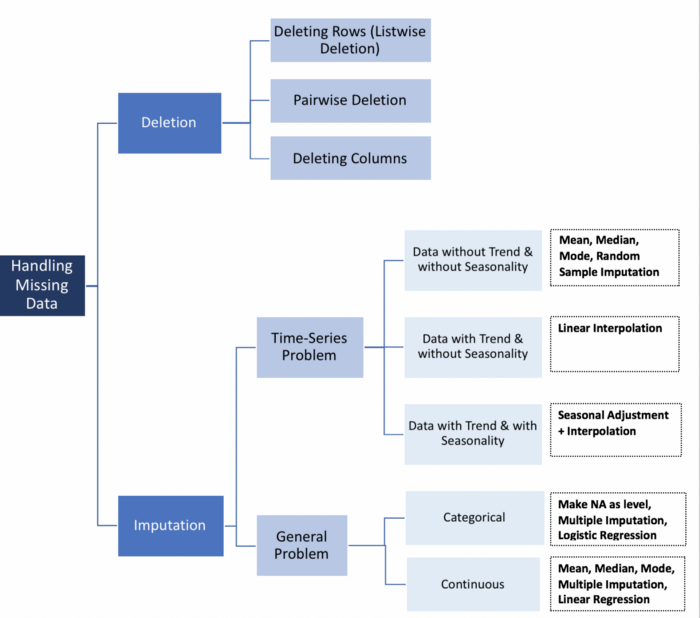
\includegraphics{pics/missingdata.png}
\end{itemize}

\hypertarget{ux7f3aux5931ux503cux7684ux5ba1ux89c6ux4e0eux6807ux8bb0}{%
\subsection{缺失值的审视与标记}\label{ux7f3aux5931ux503cux7684ux5ba1ux89c6ux4e0eux6807ux8bb0}}

\hypertarget{ux5220ux9664ux7f3aux5931ux503cux7684ux65b9ux6cd5ux53caux95eeux9898}{%
\subsection{删除缺失值的方法及问题}\label{ux5220ux9664ux7f3aux5931ux503cux7684ux65b9ux6cd5ux53caux95eeux9898}}

\begin{figure}
\centering
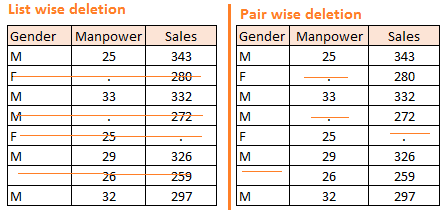
\includegraphics{pics/msdelete.png}
\caption{msdelete}
\end{figure}

\hypertarget{ux5229ux7528ux53efux9884ux6d4bux6a21ux578bux6765ux586bux8865ux7f3aux5931ux503c}{%
\subsection{利用可预测模型来填补缺失值}\label{ux5229ux7528ux53efux9884ux6d4bux6a21ux578bux6765ux586bux8865ux7f3aux5931ux503c}}

First, the missing values are filled in using median/mode imputation. Then, we mark the missing values as `Predict' and the others as training rows, which are fed into a Random Forest model trained to predict, in this case, Age based on Score. The generated prediction for that row is then filled in to produce a transformed dataset.
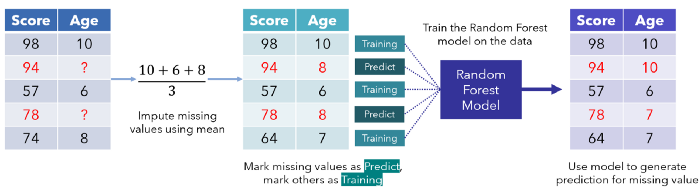
\includegraphics{pics/missforest.png}

\hypertarget{ux5904ux7406ux7f3aux5931ux503cux7684rux5305}{%
\subsection{处理缺失值的R包}\label{ux5904ux7406ux7f3aux5931ux503cux7684rux5305}}

\begin{enumerate}
\def\labelenumi{\arabic{enumi}.}
\tightlist
\item
  MICE
  (Multivariate Imputation via Chained Equations) is one of the commonly used package by R users. Creating multiple imputations as compared to a single imputation (such as mean) takes care of uncertainty in missing values.
  MICE assumes that the missing data are Missing at Random (MAR), which means that the probability that a value is missing depends only on observed value and can be predicted using them. It imputes data on a variable by variable basis by specifying an imputation model per variable.
  For example: Suppose we have X1, X2\ldots.Xk variables. If X1 has missing values, then it will be regressed on other variables X2 to Xk. The missing values in X1 will be then replaced by predictive values obtained. Similarly, if X2 has missing values, then X1, X3 to Xk variables will be used in prediction model as independent variables. Later, missing values will be replaced with predicted values.
  By default, linear regression is used to predict continuous missing values. Logistic regression is used for categorical missing values. Once this cycle is complete, multiple data sets are generated. These data sets differ only in imputed missing values. Generally, it's considered to be a good practice to build models on these data sets separately and combining their results.
\item
  Amelia
\item
  missForest
\item
  Hmisc
\item
  mi
\end{enumerate}

\hypertarget{ux5b9eux4f8b}{%
\subsection{实例}\label{ux5b9eux4f8b}}

\begin{Shaded}
\begin{Highlighting}[]
\CommentTok{\#install.packages("mice")}
\CommentTok{\#install.packages("missForest")}
\FunctionTok{library}\NormalTok{(mice)}
\end{Highlighting}
\end{Shaded}

\begin{verbatim}
## 
## Attaching package: 'mice'
\end{verbatim}

\begin{verbatim}
## The following object is masked from 'package:stats':
## 
##     filter
\end{verbatim}

\begin{verbatim}
## The following objects are masked from 'package:base':
## 
##     cbind, rbind
\end{verbatim}

\begin{Shaded}
\begin{Highlighting}[]
\FunctionTok{library}\NormalTok{(missForest)}
\end{Highlighting}
\end{Shaded}

\begin{verbatim}
## Loading required package: randomForest
\end{verbatim}

\begin{verbatim}
## randomForest 4.7-1
\end{verbatim}

\begin{verbatim}
## Type rfNews() to see new features/changes/bug fixes.
\end{verbatim}

\begin{verbatim}
## 
## Attaching package: 'randomForest'
\end{verbatim}

\begin{verbatim}
## The following object is masked from 'package:dplyr':
## 
##     combine
\end{verbatim}

\begin{verbatim}
## The following object is masked from 'package:ggplot2':
## 
##     margin
\end{verbatim}

\begin{verbatim}
## Loading required package: foreach
\end{verbatim}

\begin{verbatim}
## 
## Attaching package: 'foreach'
\end{verbatim}

\begin{verbatim}
## The following objects are masked from 'package:purrr':
## 
##     accumulate, when
\end{verbatim}

\begin{verbatim}
## Loading required package: itertools
\end{verbatim}

\begin{verbatim}
## Loading required package: iterators
\end{verbatim}

\begin{Shaded}
\begin{Highlighting}[]
\CommentTok{\#load data}
\NormalTok{data }\OtherTok{\textless{}{-}}\NormalTok{ iris }
\CommentTok{\# Get summary}
\FunctionTok{summary}\NormalTok{(data)}
\end{Highlighting}
\end{Shaded}

\begin{verbatim}
##   Sepal.Length    Sepal.Width     Petal.Length    Petal.Width   
##  Min.   :4.300   Min.   :2.000   Min.   :1.000   Min.   :0.100  
##  1st Qu.:5.100   1st Qu.:2.800   1st Qu.:1.600   1st Qu.:0.300  
##  Median :5.800   Median :3.000   Median :4.350   Median :1.300  
##  Mean   :5.843   Mean   :3.057   Mean   :3.758   Mean   :1.199  
##  3rd Qu.:6.400   3rd Qu.:3.300   3rd Qu.:5.100   3rd Qu.:1.800  
##  Max.   :7.900   Max.   :4.400   Max.   :6.900   Max.   :2.500  
##        Species  
##  setosa    :50  
##  versicolor:50  
##  virginica :50  
##                 
##                 
## 
\end{verbatim}

\begin{Shaded}
\begin{Highlighting}[]
\CommentTok{\#Generate 10\% missing values at Random}
\NormalTok{iris.mis }\OtherTok{\textless{}{-}} \FunctionTok{prodNA}\NormalTok{(data, }\AttributeTok{noNA =} \FloatTok{0.1}\NormalTok{)}
\CommentTok{\#Check missing values introduced in the data}
\FunctionTok{summary}\NormalTok{(iris.mis)}
\end{Highlighting}
\end{Shaded}

\begin{verbatim}
##   Sepal.Length    Sepal.Width     Petal.Length    Petal.Width   
##  Min.   :4.300   Min.   :2.000   Min.   :1.000   Min.   :0.100  
##  1st Qu.:5.100   1st Qu.:2.800   1st Qu.:1.600   1st Qu.:0.300  
##  Median :5.800   Median :3.000   Median :4.300   Median :1.300  
##  Mean   :5.821   Mean   :3.048   Mean   :3.747   Mean   :1.204  
##  3rd Qu.:6.325   3rd Qu.:3.300   3rd Qu.:5.100   3rd Qu.:1.800  
##  Max.   :7.900   Max.   :4.400   Max.   :6.700   Max.   :2.500  
##  NA's   :14      NA's   :17      NA's   :15      NA's   :9      
##        Species  
##  setosa    :41  
##  versicolor:46  
##  virginica :43  
##  NA's      :20  
##                 
##                 
## 
\end{verbatim}

\begin{Shaded}
\begin{Highlighting}[]
\CommentTok{\# Removing categorical data}
\NormalTok{iris.mis }\OtherTok{\textless{}{-}} \FunctionTok{subset}\NormalTok{(iris.mis, }\AttributeTok{select =} \SpecialCharTok{{-}}\FunctionTok{c}\NormalTok{(Species))}
\FunctionTok{summary}\NormalTok{(iris.mis)}
\end{Highlighting}
\end{Shaded}

\begin{verbatim}
##   Sepal.Length    Sepal.Width     Petal.Length    Petal.Width   
##  Min.   :4.300   Min.   :2.000   Min.   :1.000   Min.   :0.100  
##  1st Qu.:5.100   1st Qu.:2.800   1st Qu.:1.600   1st Qu.:0.300  
##  Median :5.800   Median :3.000   Median :4.300   Median :1.300  
##  Mean   :5.821   Mean   :3.048   Mean   :3.747   Mean   :1.204  
##  3rd Qu.:6.325   3rd Qu.:3.300   3rd Qu.:5.100   3rd Qu.:1.800  
##  Max.   :7.900   Max.   :4.400   Max.   :6.700   Max.   :2.500  
##  NA's   :14      NA's   :17      NA's   :15      NA's   :9
\end{verbatim}

\begin{Shaded}
\begin{Highlighting}[]
\FunctionTok{md.pattern}\NormalTok{(iris.mis)}
\end{Highlighting}
\end{Shaded}

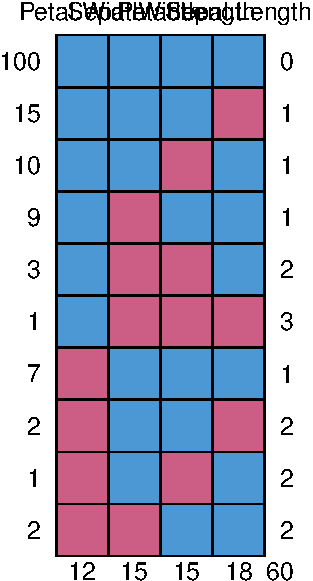
\includegraphics{03-method_files/figure-latex/mdcase-1.pdf}

\begin{verbatim}
##     Petal.Width Sepal.Length Petal.Length Sepal.Width   
## 103           1            1            1           1  0
## 11            1            1            1           0  1
## 12            1            1            0           1  1
## 1             1            1            0           0  2
## 9             1            0            1           1  1
## 4             1            0            1           0  2
## 1             1            0            0           1  2
## 8             0            1            1           1  1
## 1             0            1            0           0  3
##               9           14           15          17 55
\end{verbatim}

\begin{Shaded}
\begin{Highlighting}[]
\CommentTok{\# make it beautiful missing pattern}
\CommentTok{\#install.packages("VIM")}
\FunctionTok{library}\NormalTok{(VIM)}
\end{Highlighting}
\end{Shaded}

\begin{verbatim}
## Loading required package: colorspace
\end{verbatim}

\begin{verbatim}
## Loading required package: grid
\end{verbatim}

\begin{verbatim}
## VIM is ready to use.
\end{verbatim}

\begin{verbatim}
## Suggestions and bug-reports can be submitted at: https://github.com/statistikat/VIM/issues
\end{verbatim}

\begin{verbatim}
## 
## Attaching package: 'VIM'
\end{verbatim}

\begin{verbatim}
## The following object is masked from 'package:missForest':
## 
##     nrmse
\end{verbatim}

\begin{verbatim}
## The following object is masked from 'package:datasets':
## 
##     sleep
\end{verbatim}

\begin{Shaded}
\begin{Highlighting}[]
\NormalTok{mice\_plot }\OtherTok{\textless{}{-}} \FunctionTok{aggr}\NormalTok{(iris.mis, }\AttributeTok{col=}\FunctionTok{c}\NormalTok{(}\StringTok{\textquotesingle{}navyblue\textquotesingle{}}\NormalTok{,}\StringTok{\textquotesingle{}yellow\textquotesingle{}}\NormalTok{),}
\AttributeTok{numbers=}\ConstantTok{TRUE}\NormalTok{, }\AttributeTok{sortVars=}\ConstantTok{TRUE}\NormalTok{,}
\AttributeTok{labels=}\FunctionTok{names}\NormalTok{(iris.mis), }\AttributeTok{cex.axis=}\NormalTok{.}\DecValTok{7}\NormalTok{,}
\AttributeTok{gap=}\DecValTok{3}\NormalTok{, }\AttributeTok{ylab=}\FunctionTok{c}\NormalTok{(}\StringTok{"Missing data"}\NormalTok{,}\StringTok{"Pattern"}\NormalTok{))}
\end{Highlighting}
\end{Shaded}

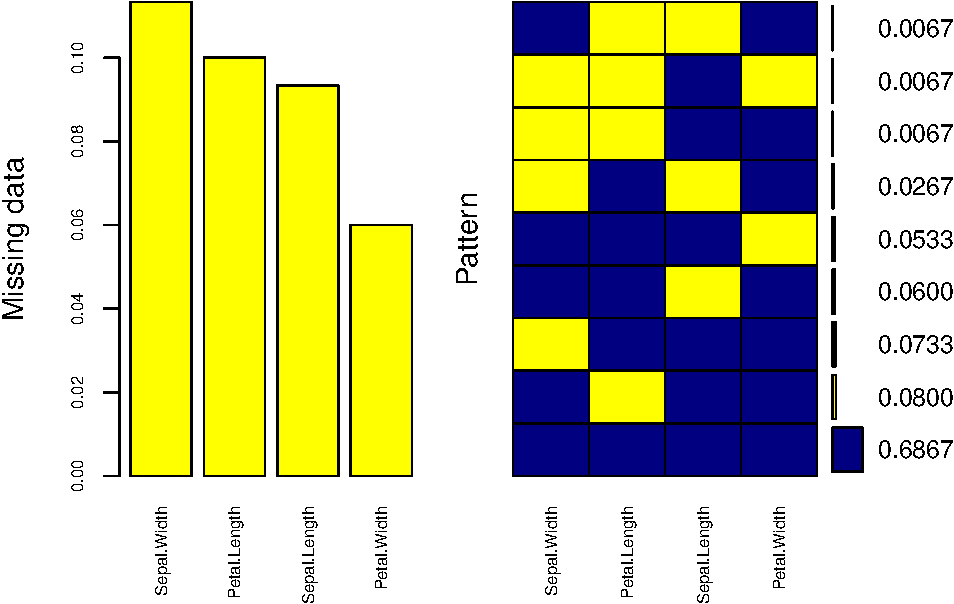
\includegraphics{03-method_files/figure-latex/mdcase-2.pdf}

\begin{verbatim}
## 
##  Variables sorted by number of missings: 
##      Variable      Count
##   Sepal.Width 0.11333333
##  Petal.Length 0.10000000
##  Sepal.Length 0.09333333
##   Petal.Width 0.06000000
\end{verbatim}

\begin{Shaded}
\begin{Highlighting}[]
\CommentTok{\# impute the missing data using mice}
\NormalTok{imputed\_Data }\OtherTok{\textless{}{-}} \FunctionTok{mice}\NormalTok{(iris.mis, }\AttributeTok{m=}\DecValTok{5}\NormalTok{, }\AttributeTok{maxit =} \DecValTok{50}\NormalTok{, }\AttributeTok{method =} \StringTok{\textquotesingle{}pmm\textquotesingle{}}\NormalTok{, }\AttributeTok{seed =} \DecValTok{500}\NormalTok{)}
\end{Highlighting}
\end{Shaded}

\begin{verbatim}
## 
##  iter imp variable
##   1   1  Sepal.Length  Sepal.Width  Petal.Length  Petal.Width
##   1   2  Sepal.Length  Sepal.Width  Petal.Length  Petal.Width
##   1   3  Sepal.Length  Sepal.Width  Petal.Length  Petal.Width
##   1   4  Sepal.Length  Sepal.Width  Petal.Length  Petal.Width
##   1   5  Sepal.Length  Sepal.Width  Petal.Length  Petal.Width
##   2   1  Sepal.Length  Sepal.Width  Petal.Length  Petal.Width
##   2   2  Sepal.Length  Sepal.Width  Petal.Length  Petal.Width
##   2   3  Sepal.Length  Sepal.Width  Petal.Length  Petal.Width
##   2   4  Sepal.Length  Sepal.Width  Petal.Length  Petal.Width
##   2   5  Sepal.Length  Sepal.Width  Petal.Length  Petal.Width
##   3   1  Sepal.Length  Sepal.Width  Petal.Length  Petal.Width
##   3   2  Sepal.Length  Sepal.Width  Petal.Length  Petal.Width
##   3   3  Sepal.Length  Sepal.Width  Petal.Length  Petal.Width
##   3   4  Sepal.Length  Sepal.Width  Petal.Length  Petal.Width
##   3   5  Sepal.Length  Sepal.Width  Petal.Length  Petal.Width
##   4   1  Sepal.Length  Sepal.Width  Petal.Length  Petal.Width
##   4   2  Sepal.Length  Sepal.Width  Petal.Length  Petal.Width
##   4   3  Sepal.Length  Sepal.Width  Petal.Length  Petal.Width
##   4   4  Sepal.Length  Sepal.Width  Petal.Length  Petal.Width
##   4   5  Sepal.Length  Sepal.Width  Petal.Length  Petal.Width
##   5   1  Sepal.Length  Sepal.Width  Petal.Length  Petal.Width
##   5   2  Sepal.Length  Sepal.Width  Petal.Length  Petal.Width
##   5   3  Sepal.Length  Sepal.Width  Petal.Length  Petal.Width
##   5   4  Sepal.Length  Sepal.Width  Petal.Length  Petal.Width
##   5   5  Sepal.Length  Sepal.Width  Petal.Length  Petal.Width
##   6   1  Sepal.Length  Sepal.Width  Petal.Length  Petal.Width
##   6   2  Sepal.Length  Sepal.Width  Petal.Length  Petal.Width
##   6   3  Sepal.Length  Sepal.Width  Petal.Length  Petal.Width
##   6   4  Sepal.Length  Sepal.Width  Petal.Length  Petal.Width
##   6   5  Sepal.Length  Sepal.Width  Petal.Length  Petal.Width
##   7   1  Sepal.Length  Sepal.Width  Petal.Length  Petal.Width
##   7   2  Sepal.Length  Sepal.Width  Petal.Length  Petal.Width
##   7   3  Sepal.Length  Sepal.Width  Petal.Length  Petal.Width
##   7   4  Sepal.Length  Sepal.Width  Petal.Length  Petal.Width
##   7   5  Sepal.Length  Sepal.Width  Petal.Length  Petal.Width
##   8   1  Sepal.Length  Sepal.Width  Petal.Length  Petal.Width
##   8   2  Sepal.Length  Sepal.Width  Petal.Length  Petal.Width
##   8   3  Sepal.Length  Sepal.Width  Petal.Length  Petal.Width
##   8   4  Sepal.Length  Sepal.Width  Petal.Length  Petal.Width
##   8   5  Sepal.Length  Sepal.Width  Petal.Length  Petal.Width
##   9   1  Sepal.Length  Sepal.Width  Petal.Length  Petal.Width
##   9   2  Sepal.Length  Sepal.Width  Petal.Length  Petal.Width
##   9   3  Sepal.Length  Sepal.Width  Petal.Length  Petal.Width
##   9   4  Sepal.Length  Sepal.Width  Petal.Length  Petal.Width
##   9   5  Sepal.Length  Sepal.Width  Petal.Length  Petal.Width
##   10   1  Sepal.Length  Sepal.Width  Petal.Length  Petal.Width
##   10   2  Sepal.Length  Sepal.Width  Petal.Length  Petal.Width
##   10   3  Sepal.Length  Sepal.Width  Petal.Length  Petal.Width
##   10   4  Sepal.Length  Sepal.Width  Petal.Length  Petal.Width
##   10   5  Sepal.Length  Sepal.Width  Petal.Length  Petal.Width
##   11   1  Sepal.Length  Sepal.Width  Petal.Length  Petal.Width
##   11   2  Sepal.Length  Sepal.Width  Petal.Length  Petal.Width
##   11   3  Sepal.Length  Sepal.Width  Petal.Length  Petal.Width
##   11   4  Sepal.Length  Sepal.Width  Petal.Length  Petal.Width
##   11   5  Sepal.Length  Sepal.Width  Petal.Length  Petal.Width
##   12   1  Sepal.Length  Sepal.Width  Petal.Length  Petal.Width
##   12   2  Sepal.Length  Sepal.Width  Petal.Length  Petal.Width
##   12   3  Sepal.Length  Sepal.Width  Petal.Length  Petal.Width
##   12   4  Sepal.Length  Sepal.Width  Petal.Length  Petal.Width
##   12   5  Sepal.Length  Sepal.Width  Petal.Length  Petal.Width
##   13   1  Sepal.Length  Sepal.Width  Petal.Length  Petal.Width
##   13   2  Sepal.Length  Sepal.Width  Petal.Length  Petal.Width
##   13   3  Sepal.Length  Sepal.Width  Petal.Length  Petal.Width
##   13   4  Sepal.Length  Sepal.Width  Petal.Length  Petal.Width
##   13   5  Sepal.Length  Sepal.Width  Petal.Length  Petal.Width
##   14   1  Sepal.Length  Sepal.Width  Petal.Length  Petal.Width
##   14   2  Sepal.Length  Sepal.Width  Petal.Length  Petal.Width
##   14   3  Sepal.Length  Sepal.Width  Petal.Length  Petal.Width
##   14   4  Sepal.Length  Sepal.Width  Petal.Length  Petal.Width
##   14   5  Sepal.Length  Sepal.Width  Petal.Length  Petal.Width
##   15   1  Sepal.Length  Sepal.Width  Petal.Length  Petal.Width
##   15   2  Sepal.Length  Sepal.Width  Petal.Length  Petal.Width
##   15   3  Sepal.Length  Sepal.Width  Petal.Length  Petal.Width
##   15   4  Sepal.Length  Sepal.Width  Petal.Length  Petal.Width
##   15   5  Sepal.Length  Sepal.Width  Petal.Length  Petal.Width
##   16   1  Sepal.Length  Sepal.Width  Petal.Length  Petal.Width
##   16   2  Sepal.Length  Sepal.Width  Petal.Length  Petal.Width
##   16   3  Sepal.Length  Sepal.Width  Petal.Length  Petal.Width
##   16   4  Sepal.Length  Sepal.Width  Petal.Length  Petal.Width
##   16   5  Sepal.Length  Sepal.Width  Petal.Length  Petal.Width
##   17   1  Sepal.Length  Sepal.Width  Petal.Length  Petal.Width
##   17   2  Sepal.Length  Sepal.Width  Petal.Length  Petal.Width
##   17   3  Sepal.Length  Sepal.Width  Petal.Length  Petal.Width
##   17   4  Sepal.Length  Sepal.Width  Petal.Length  Petal.Width
##   17   5  Sepal.Length  Sepal.Width  Petal.Length  Petal.Width
##   18   1  Sepal.Length  Sepal.Width  Petal.Length  Petal.Width
##   18   2  Sepal.Length  Sepal.Width  Petal.Length  Petal.Width
##   18   3  Sepal.Length  Sepal.Width  Petal.Length  Petal.Width
##   18   4  Sepal.Length  Sepal.Width  Petal.Length  Petal.Width
##   18   5  Sepal.Length  Sepal.Width  Petal.Length  Petal.Width
##   19   1  Sepal.Length  Sepal.Width  Petal.Length  Petal.Width
##   19   2  Sepal.Length  Sepal.Width  Petal.Length  Petal.Width
##   19   3  Sepal.Length  Sepal.Width  Petal.Length  Petal.Width
##   19   4  Sepal.Length  Sepal.Width  Petal.Length  Petal.Width
##   19   5  Sepal.Length  Sepal.Width  Petal.Length  Petal.Width
##   20   1  Sepal.Length  Sepal.Width  Petal.Length  Petal.Width
##   20   2  Sepal.Length  Sepal.Width  Petal.Length  Petal.Width
##   20   3  Sepal.Length  Sepal.Width  Petal.Length  Petal.Width
##   20   4  Sepal.Length  Sepal.Width  Petal.Length  Petal.Width
##   20   5  Sepal.Length  Sepal.Width  Petal.Length  Petal.Width
##   21   1  Sepal.Length  Sepal.Width  Petal.Length  Petal.Width
##   21   2  Sepal.Length  Sepal.Width  Petal.Length  Petal.Width
##   21   3  Sepal.Length  Sepal.Width  Petal.Length  Petal.Width
##   21   4  Sepal.Length  Sepal.Width  Petal.Length  Petal.Width
##   21   5  Sepal.Length  Sepal.Width  Petal.Length  Petal.Width
##   22   1  Sepal.Length  Sepal.Width  Petal.Length  Petal.Width
##   22   2  Sepal.Length  Sepal.Width  Petal.Length  Petal.Width
##   22   3  Sepal.Length  Sepal.Width  Petal.Length  Petal.Width
##   22   4  Sepal.Length  Sepal.Width  Petal.Length  Petal.Width
##   22   5  Sepal.Length  Sepal.Width  Petal.Length  Petal.Width
##   23   1  Sepal.Length  Sepal.Width  Petal.Length  Petal.Width
##   23   2  Sepal.Length  Sepal.Width  Petal.Length  Petal.Width
##   23   3  Sepal.Length  Sepal.Width  Petal.Length  Petal.Width
##   23   4  Sepal.Length  Sepal.Width  Petal.Length  Petal.Width
##   23   5  Sepal.Length  Sepal.Width  Petal.Length  Petal.Width
##   24   1  Sepal.Length  Sepal.Width  Petal.Length  Petal.Width
##   24   2  Sepal.Length  Sepal.Width  Petal.Length  Petal.Width
##   24   3  Sepal.Length  Sepal.Width  Petal.Length  Petal.Width
##   24   4  Sepal.Length  Sepal.Width  Petal.Length  Petal.Width
##   24   5  Sepal.Length  Sepal.Width  Petal.Length  Petal.Width
##   25   1  Sepal.Length  Sepal.Width  Petal.Length  Petal.Width
##   25   2  Sepal.Length  Sepal.Width  Petal.Length  Petal.Width
##   25   3  Sepal.Length  Sepal.Width  Petal.Length  Petal.Width
##   25   4  Sepal.Length  Sepal.Width  Petal.Length  Petal.Width
##   25   5  Sepal.Length  Sepal.Width  Petal.Length  Petal.Width
##   26   1  Sepal.Length  Sepal.Width  Petal.Length  Petal.Width
##   26   2  Sepal.Length  Sepal.Width  Petal.Length  Petal.Width
##   26   3  Sepal.Length  Sepal.Width  Petal.Length  Petal.Width
##   26   4  Sepal.Length  Sepal.Width  Petal.Length  Petal.Width
##   26   5  Sepal.Length  Sepal.Width  Petal.Length  Petal.Width
##   27   1  Sepal.Length  Sepal.Width  Petal.Length  Petal.Width
##   27   2  Sepal.Length  Sepal.Width  Petal.Length  Petal.Width
##   27   3  Sepal.Length  Sepal.Width  Petal.Length  Petal.Width
##   27   4  Sepal.Length  Sepal.Width  Petal.Length  Petal.Width
##   27   5  Sepal.Length  Sepal.Width  Petal.Length  Petal.Width
##   28   1  Sepal.Length  Sepal.Width  Petal.Length  Petal.Width
##   28   2  Sepal.Length  Sepal.Width  Petal.Length  Petal.Width
##   28   3  Sepal.Length  Sepal.Width  Petal.Length  Petal.Width
##   28   4  Sepal.Length  Sepal.Width  Petal.Length  Petal.Width
##   28   5  Sepal.Length  Sepal.Width  Petal.Length  Petal.Width
##   29   1  Sepal.Length  Sepal.Width  Petal.Length  Petal.Width
##   29   2  Sepal.Length  Sepal.Width  Petal.Length  Petal.Width
##   29   3  Sepal.Length  Sepal.Width  Petal.Length  Petal.Width
##   29   4  Sepal.Length  Sepal.Width  Petal.Length  Petal.Width
##   29   5  Sepal.Length  Sepal.Width  Petal.Length  Petal.Width
##   30   1  Sepal.Length  Sepal.Width  Petal.Length  Petal.Width
##   30   2  Sepal.Length  Sepal.Width  Petal.Length  Petal.Width
##   30   3  Sepal.Length  Sepal.Width  Petal.Length  Petal.Width
##   30   4  Sepal.Length  Sepal.Width  Petal.Length  Petal.Width
##   30   5  Sepal.Length  Sepal.Width  Petal.Length  Petal.Width
##   31   1  Sepal.Length  Sepal.Width  Petal.Length  Petal.Width
##   31   2  Sepal.Length  Sepal.Width  Petal.Length  Petal.Width
##   31   3  Sepal.Length  Sepal.Width  Petal.Length  Petal.Width
##   31   4  Sepal.Length  Sepal.Width  Petal.Length  Petal.Width
##   31   5  Sepal.Length  Sepal.Width  Petal.Length  Petal.Width
##   32   1  Sepal.Length  Sepal.Width  Petal.Length  Petal.Width
##   32   2  Sepal.Length  Sepal.Width  Petal.Length  Petal.Width
##   32   3  Sepal.Length  Sepal.Width  Petal.Length  Petal.Width
##   32   4  Sepal.Length  Sepal.Width  Petal.Length  Petal.Width
##   32   5  Sepal.Length  Sepal.Width  Petal.Length  Petal.Width
##   33   1  Sepal.Length  Sepal.Width  Petal.Length  Petal.Width
##   33   2  Sepal.Length  Sepal.Width  Petal.Length  Petal.Width
##   33   3  Sepal.Length  Sepal.Width  Petal.Length  Petal.Width
##   33   4  Sepal.Length  Sepal.Width  Petal.Length  Petal.Width
##   33   5  Sepal.Length  Sepal.Width  Petal.Length  Petal.Width
##   34   1  Sepal.Length  Sepal.Width  Petal.Length  Petal.Width
##   34   2  Sepal.Length  Sepal.Width  Petal.Length  Petal.Width
##   34   3  Sepal.Length  Sepal.Width  Petal.Length  Petal.Width
##   34   4  Sepal.Length  Sepal.Width  Petal.Length  Petal.Width
##   34   5  Sepal.Length  Sepal.Width  Petal.Length  Petal.Width
##   35   1  Sepal.Length  Sepal.Width  Petal.Length  Petal.Width
##   35   2  Sepal.Length  Sepal.Width  Petal.Length  Petal.Width
##   35   3  Sepal.Length  Sepal.Width  Petal.Length  Petal.Width
##   35   4  Sepal.Length  Sepal.Width  Petal.Length  Petal.Width
##   35   5  Sepal.Length  Sepal.Width  Petal.Length  Petal.Width
##   36   1  Sepal.Length  Sepal.Width  Petal.Length  Petal.Width
##   36   2  Sepal.Length  Sepal.Width  Petal.Length  Petal.Width
##   36   3  Sepal.Length  Sepal.Width  Petal.Length  Petal.Width
##   36   4  Sepal.Length  Sepal.Width  Petal.Length  Petal.Width
##   36   5  Sepal.Length  Sepal.Width  Petal.Length  Petal.Width
##   37   1  Sepal.Length  Sepal.Width  Petal.Length  Petal.Width
##   37   2  Sepal.Length  Sepal.Width  Petal.Length  Petal.Width
##   37   3  Sepal.Length  Sepal.Width  Petal.Length  Petal.Width
##   37   4  Sepal.Length  Sepal.Width  Petal.Length  Petal.Width
##   37   5  Sepal.Length  Sepal.Width  Petal.Length  Petal.Width
##   38   1  Sepal.Length  Sepal.Width  Petal.Length  Petal.Width
##   38   2  Sepal.Length  Sepal.Width  Petal.Length  Petal.Width
##   38   3  Sepal.Length  Sepal.Width  Petal.Length  Petal.Width
##   38   4  Sepal.Length  Sepal.Width  Petal.Length  Petal.Width
##   38   5  Sepal.Length  Sepal.Width  Petal.Length  Petal.Width
##   39   1  Sepal.Length  Sepal.Width  Petal.Length  Petal.Width
##   39   2  Sepal.Length  Sepal.Width  Petal.Length  Petal.Width
##   39   3  Sepal.Length  Sepal.Width  Petal.Length  Petal.Width
##   39   4  Sepal.Length  Sepal.Width  Petal.Length  Petal.Width
##   39   5  Sepal.Length  Sepal.Width  Petal.Length  Petal.Width
##   40   1  Sepal.Length  Sepal.Width  Petal.Length  Petal.Width
##   40   2  Sepal.Length  Sepal.Width  Petal.Length  Petal.Width
##   40   3  Sepal.Length  Sepal.Width  Petal.Length  Petal.Width
##   40   4  Sepal.Length  Sepal.Width  Petal.Length  Petal.Width
##   40   5  Sepal.Length  Sepal.Width  Petal.Length  Petal.Width
##   41   1  Sepal.Length  Sepal.Width  Petal.Length  Petal.Width
##   41   2  Sepal.Length  Sepal.Width  Petal.Length  Petal.Width
##   41   3  Sepal.Length  Sepal.Width  Petal.Length  Petal.Width
##   41   4  Sepal.Length  Sepal.Width  Petal.Length  Petal.Width
##   41   5  Sepal.Length  Sepal.Width  Petal.Length  Petal.Width
##   42   1  Sepal.Length  Sepal.Width  Petal.Length  Petal.Width
##   42   2  Sepal.Length  Sepal.Width  Petal.Length  Petal.Width
##   42   3  Sepal.Length  Sepal.Width  Petal.Length  Petal.Width
##   42   4  Sepal.Length  Sepal.Width  Petal.Length  Petal.Width
##   42   5  Sepal.Length  Sepal.Width  Petal.Length  Petal.Width
##   43   1  Sepal.Length  Sepal.Width  Petal.Length  Petal.Width
##   43   2  Sepal.Length  Sepal.Width  Petal.Length  Petal.Width
##   43   3  Sepal.Length  Sepal.Width  Petal.Length  Petal.Width
##   43   4  Sepal.Length  Sepal.Width  Petal.Length  Petal.Width
##   43   5  Sepal.Length  Sepal.Width  Petal.Length  Petal.Width
##   44   1  Sepal.Length  Sepal.Width  Petal.Length  Petal.Width
##   44   2  Sepal.Length  Sepal.Width  Petal.Length  Petal.Width
##   44   3  Sepal.Length  Sepal.Width  Petal.Length  Petal.Width
##   44   4  Sepal.Length  Sepal.Width  Petal.Length  Petal.Width
##   44   5  Sepal.Length  Sepal.Width  Petal.Length  Petal.Width
##   45   1  Sepal.Length  Sepal.Width  Petal.Length  Petal.Width
##   45   2  Sepal.Length  Sepal.Width  Petal.Length  Petal.Width
##   45   3  Sepal.Length  Sepal.Width  Petal.Length  Petal.Width
##   45   4  Sepal.Length  Sepal.Width  Petal.Length  Petal.Width
##   45   5  Sepal.Length  Sepal.Width  Petal.Length  Petal.Width
##   46   1  Sepal.Length  Sepal.Width  Petal.Length  Petal.Width
##   46   2  Sepal.Length  Sepal.Width  Petal.Length  Petal.Width
##   46   3  Sepal.Length  Sepal.Width  Petal.Length  Petal.Width
##   46   4  Sepal.Length  Sepal.Width  Petal.Length  Petal.Width
##   46   5  Sepal.Length  Sepal.Width  Petal.Length  Petal.Width
##   47   1  Sepal.Length  Sepal.Width  Petal.Length  Petal.Width
##   47   2  Sepal.Length  Sepal.Width  Petal.Length  Petal.Width
##   47   3  Sepal.Length  Sepal.Width  Petal.Length  Petal.Width
##   47   4  Sepal.Length  Sepal.Width  Petal.Length  Petal.Width
##   47   5  Sepal.Length  Sepal.Width  Petal.Length  Petal.Width
##   48   1  Sepal.Length  Sepal.Width  Petal.Length  Petal.Width
##   48   2  Sepal.Length  Sepal.Width  Petal.Length  Petal.Width
##   48   3  Sepal.Length  Sepal.Width  Petal.Length  Petal.Width
##   48   4  Sepal.Length  Sepal.Width  Petal.Length  Petal.Width
##   48   5  Sepal.Length  Sepal.Width  Petal.Length  Petal.Width
##   49   1  Sepal.Length  Sepal.Width  Petal.Length  Petal.Width
##   49   2  Sepal.Length  Sepal.Width  Petal.Length  Petal.Width
##   49   3  Sepal.Length  Sepal.Width  Petal.Length  Petal.Width
##   49   4  Sepal.Length  Sepal.Width  Petal.Length  Petal.Width
##   49   5  Sepal.Length  Sepal.Width  Petal.Length  Petal.Width
##   50   1  Sepal.Length  Sepal.Width  Petal.Length  Petal.Width
##   50   2  Sepal.Length  Sepal.Width  Petal.Length  Petal.Width
##   50   3  Sepal.Length  Sepal.Width  Petal.Length  Petal.Width
##   50   4  Sepal.Length  Sepal.Width  Petal.Length  Petal.Width
##   50   5  Sepal.Length  Sepal.Width  Petal.Length  Petal.Width
\end{verbatim}

\begin{Shaded}
\begin{Highlighting}[]
\CommentTok{\#m — Refers to 5 imputed data sets;maxit — Refers to no. of iterations taken to impute missing values;method — Refers to method used in imputation. we used predictive mean matching}
\FunctionTok{summary}\NormalTok{(imputed\_Data)}
\end{Highlighting}
\end{Shaded}

\begin{verbatim}
## Class: mids
## Number of multiple imputations:  5 
## Imputation methods:
## Sepal.Length  Sepal.Width Petal.Length  Petal.Width 
##        "pmm"        "pmm"        "pmm"        "pmm" 
## PredictorMatrix:
##              Sepal.Length Sepal.Width Petal.Length Petal.Width
## Sepal.Length            0           1            1           1
## Sepal.Width             1           0            1           1
## Petal.Length            1           1            0           1
## Petal.Width             1           1            1           0
\end{verbatim}

\begin{Shaded}
\begin{Highlighting}[]
\CommentTok{\#check imputed values}
\NormalTok{imputed\_Data}\SpecialCharTok{$}\NormalTok{imp}\SpecialCharTok{$}\NormalTok{Sepal.Width}
\end{Highlighting}
\end{Shaded}

\begin{verbatim}
##       1   2   3   4   5
## 3   3.6 3.1 3.8 3.2 3.0
## 5   3.5 3.8 3.1 3.1 3.0
## 19  3.7 3.9 3.5 3.7 3.5
## 23  3.3 3.4 3.2 3.4 3.8
## 30  3.0 3.0 3.6 3.0 3.3
## 32  3.5 3.9 3.3 3.3 3.5
## 34  4.1 3.3 3.5 3.8 3.0
## 55  2.8 3.1 3.1 3.3 3.2
## 68  2.8 2.4 2.5 3.0 2.4
## 75  2.8 3.1 3.2 2.5 3.0
## 88  2.8 2.7 3.1 2.6 2.2
## 95  2.5 2.9 2.3 2.8 2.5
## 104 2.6 2.8 2.7 3.0 2.2
## 118 3.4 3.0 3.0 3.0 3.0
## 123 3.4 3.3 2.0 2.6 2.6
## 129 2.3 3.0 3.3 3.4 2.5
## 147 3.3 3.0 2.5 3.4 2.5
\end{verbatim}

\begin{Shaded}
\begin{Highlighting}[]
\CommentTok{\#get complete data ( 2nd out of 5)}
\NormalTok{completeData }\OtherTok{\textless{}{-}} \FunctionTok{complete}\NormalTok{(imputed\_Data,}\DecValTok{2}\NormalTok{)}
\CommentTok{\#build predictive model}
\FunctionTok{library}\NormalTok{(dplyr)}
\NormalTok{fit }\OtherTok{\textless{}{-}} \FunctionTok{with}\NormalTok{(}\AttributeTok{data =}\NormalTok{ iris.mis, }\AttributeTok{exp =} \FunctionTok{lm}\NormalTok{(Sepal.Width }\SpecialCharTok{\textasciitilde{}}\NormalTok{ Sepal.Length }\SpecialCharTok{+}\NormalTok{ Petal.Width))}
\CommentTok{\#combine results of all 5 models}
\CommentTok{\#combine \textless{}{-} pool(fit)}
\FunctionTok{summary}\NormalTok{(fit)}
\end{Highlighting}
\end{Shaded}

\begin{verbatim}
## 
## Call:
## lm(formula = Sepal.Width ~ Sepal.Length + Petal.Width)
## 
## Residuals:
##      Min       1Q   Median       3Q      Max 
## -0.99024 -0.23721 -0.00313  0.22600  1.02767 
## 
## Coefficients:
##              Estimate Std. Error t value Pr(>|t|)    
## (Intercept)   2.02653    0.38337   5.286 6.24e-07 ***
## Sepal.Length  0.26676    0.07830   3.407 0.000913 ***
## Petal.Width  -0.43687    0.08227  -5.310 5.61e-07 ***
## ---
## Signif. codes:  0 '***' 0.001 '**' 0.01 '*' 0.05 '.' 0.1 ' ' 1
## 
## Residual standard error: 0.3852 on 112 degrees of freedom
##   (35 observations deleted due to missingness)
## Multiple R-squared:  0.2154, Adjusted R-squared:  0.2014 
## F-statistic: 15.38 on 2 and 112 DF,  p-value: 1.255e-06
\end{verbatim}

\hypertarget{ux6709ux76d1ux7763ux5b66ux4e60ux6982ux8bba}{%
\chapter{有监督学习概论}\label{ux6709ux76d1ux7763ux5b66ux4e60ux6982ux8bba}}

Some \emph{significant} applications are demonstrated in this chapter.

\hypertarget{example-one}{%
\section{Example one}\label{example-one}}

\hypertarget{example-two}{%
\section{Example two}\label{example-two}}

\hypertarget{final-words}{%
\chapter{Final Words}\label{final-words}}

We have finished a nice book.

\hypertarget{logisticux56deux5f52}{%
\chapter{Logistic回归}\label{logisticux56deux5f52}}

This is an R Markdown document. Markdown is a simple formatting syntax for authoring HTML, PDF, and MS Word documents. For more details on using R Markdown see \url{http://rmarkdown.rstudio.com}.

When you click the \textbf{Knit} button a document will be generated that includes both content as well as the output of any embedded R code chunks within the document. You can embed an R code chunk like this:

\begin{Shaded}
\begin{Highlighting}[]
\FunctionTok{summary}\NormalTok{(cars)}
\end{Highlighting}
\end{Shaded}

\begin{verbatim}
##      speed           dist       
##  Min.   : 4.0   Min.   :  2.00  
##  1st Qu.:12.0   1st Qu.: 26.00  
##  Median :15.0   Median : 36.00  
##  Mean   :15.4   Mean   : 42.98  
##  3rd Qu.:19.0   3rd Qu.: 56.00  
##  Max.   :25.0   Max.   :120.00
\end{verbatim}

\hypertarget{including-plots}{%
\section{Including Plots}\label{including-plots}}

You can also embed plots, for example:

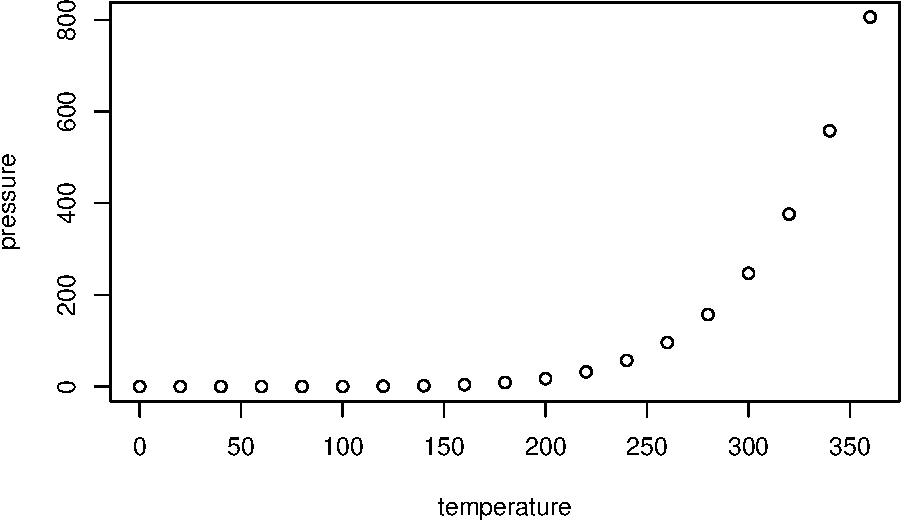
\includegraphics{07-ref_files/figure-latex/pressure-1.pdf}

Note that the \texttt{echo\ =\ FALSE} parameter was added to the code chunk to prevent printing of the R code that generated the plot.

  \bibliography{book.bib,packages.bib}

\end{document}
